\section{Content analysis}

\subsection{Homepage contents}

\subsubsection{General consideration}

Oltre a quello che è già stato detto precedentemente, la struttura della 
homepage è molto chiara e tutti gli elementi sono sufficientemente 
spaziati tra loro. La dimensione del carattere è grande, con lo scopo di 
catturare l'attenzione dell'utente. Sono presenti degli elementi grafici 
che rendono la pagina interattiva e la arrichiscono dal punto di vista dei 
contenuti. Inoltre, è presente un'immagine animata con lo scopo di 
illustrare le diverse possibilità di deposito di denaro. È una buona 
strategia perchè si evita di scrivere del testo lungo per spiegare le 
diverse possibilità di deposito offerte dal prodotto. Quindi, si mantiene 
la pulizia della sezione, in concordia alle altre. 

\subsubsection{Main menu}

Come detto precedentemente, il menù principale è posto in una posizione 
ideale (fig. \ref{fig:main-menu}). Tuttavia, manca uno strumento di 
fondamentale importanza: la ricerca. A primo impatto un utente non avrebbe 
modo di effettuare una ricerca tra i contenuti del sito. Questo rappresenta 
un grande svantaggio, che verrà esaminato in modo più approfondito 
successivamente.

\subsubsection{Footer}

Il footer del sito web è illustrato nella figura \ref{fig:footer}. Questa 
sezione è suddiviso in due parti principali:
\begin{itemize}
  \item Nella parte superiore, vi sono quattro colonne:
  \begin{itemize}
    \item Nella prima colonna sono elencati tutti i prodotti sviluppati 
    dall'azienda;

    \item Nella seconda colonna vengono elencate una serie di pagine che 
    illustrano delle guide sia generiche (ad esempio, 
    \textit{Inizia da qui}) che specifiche (ad esempio, 
    \textit{Comprare Bitcoin}). È possibile trovare un ridondanza, ovvero, 
    la voce \textit{Inizia da qui} e \textit{Young Platform Academy} della 
    prima colonna. Infatti, queste voci puntano alla medesima pagina;

    \item Nella terza colonna vi sono una serie di voci che puntano a delle 
    pagine che trattano contenuti strettamente collegati all'azienda di per 
    sè. Per quanto riguarda la voce \textit{I nostri prodotti}, penso che 
    sarebbe stato più coerente inserirla nella prima colonna. Tale voce 
    reindirizza ad una pagina che illustra in modo sintetico ed efficace 
    i vari prodotti. La voce \textit{Perchè Young Platform} punta ad una 
    pagina che fornisce delle motivazioni per cui utilizzare i loro 
    prodotti e di usufruire del loro ecosistema. Ritengo che questa pagina 
    ha una certa importanza ai fini di convicere gli utenti (sia principianti 
    che esperti) ad utilizzare i prodotti. Quindi, trovo che la posizione di 
    questa voce è errata, in quanto il contenuto di tale pagina ha una certa 
    importanza;

    \item Nella quarta colonna vi sono una serie di voci che reindirizzano a 
    delle pagine i cui contenuti sono molto importanti:
    \begin{itemize}
      \item \textit{Centro di Supporto}: questa voce reindirizza alla 
      medesima pagina puntata dalla voce \textit{Supporto} del menù 
      principale (fig. \ref{fig:main-menu});

      \item \textit{Commissioni e Prezzi}: reindirizza ad una pagina che 
      spiega in modo sintetico ed esaustivo le varie commissioni che 
      vengono applicate alle varie azioni che possono essere effettute con 
      i vari prodotti;

      \item \textit{FAQ *}: queste 4 voci raccolgono una serie di domande 
      frequenti che riguardano diversi argomenti (tasse, compravendita, 
      commissioni e \textit{earning wallet}). Trovo che questa suddivisione 
      non dovesse essere suddivisa per voci ma dovessero essere suddivise in 
      una pagina unica. Ritengo che per l'utente sia più utile avere accesso 
      a tutte le FAQ in una unica pagina. La suddivisione delle FAQ per 
      argomento è utile, ma non come è stata implementata nel sito. Inoltre, 
      è assente uno strumento di ricerca nelle FAQ, il che rappresenta uno 
      svantaggio.
    \end{itemize}
  \end{itemize}

  \item Nella parte inferiore, vi sono il logo e i dati legali dell'azienda, 
  un piccolo menù per la selezione della lingua (italiano, inglese e 
  francese), i link per scarire le applicazioni negli store e i link dei 
  vari social network.
\end{itemize}

\subsection{Internal pages contents}

Per quanto riguarda le pagine interne, gli assi obbligatori sono 
\textit{Who} e \textit{What}. Gli altri assi sono opzionali. In particolare, 
gli assi \textit{Where} e \textit{Why}, pur essendo opzionali, sono 
fortemente consigliati.

\subsubsection{Products page}

La pagina a cui si fa riferimento è raggiungibile al seguente indirizzo 
\href{https://youngplatform.com/young-world/}{https://youngplatform.com/young-world/}.

\paragraph{What}

In questa pagina è possibile comprendere chiaramente che cosa viene offerto. 
Fin dal titolo ad inizio pagina permette di capire che verranno illustrati 
i vari prodotti dell'azienda e le loro differenze. Nella prima sezione 
(fig. \ref{fig:products-page-1}), viene esplicitato l'obiettivo del 
contenuto della pagina. Nelle altre due sezioni 
(fig. \ref{fig:products-page-2} and \ref{fig:products-page-3}) si 
illustrano le differenze tra i vari prodotti, in modo da guidare l'utente 
verso il prodotto più adatto alle sue esigenze. 
\begin{figure}[H]
  \centering
  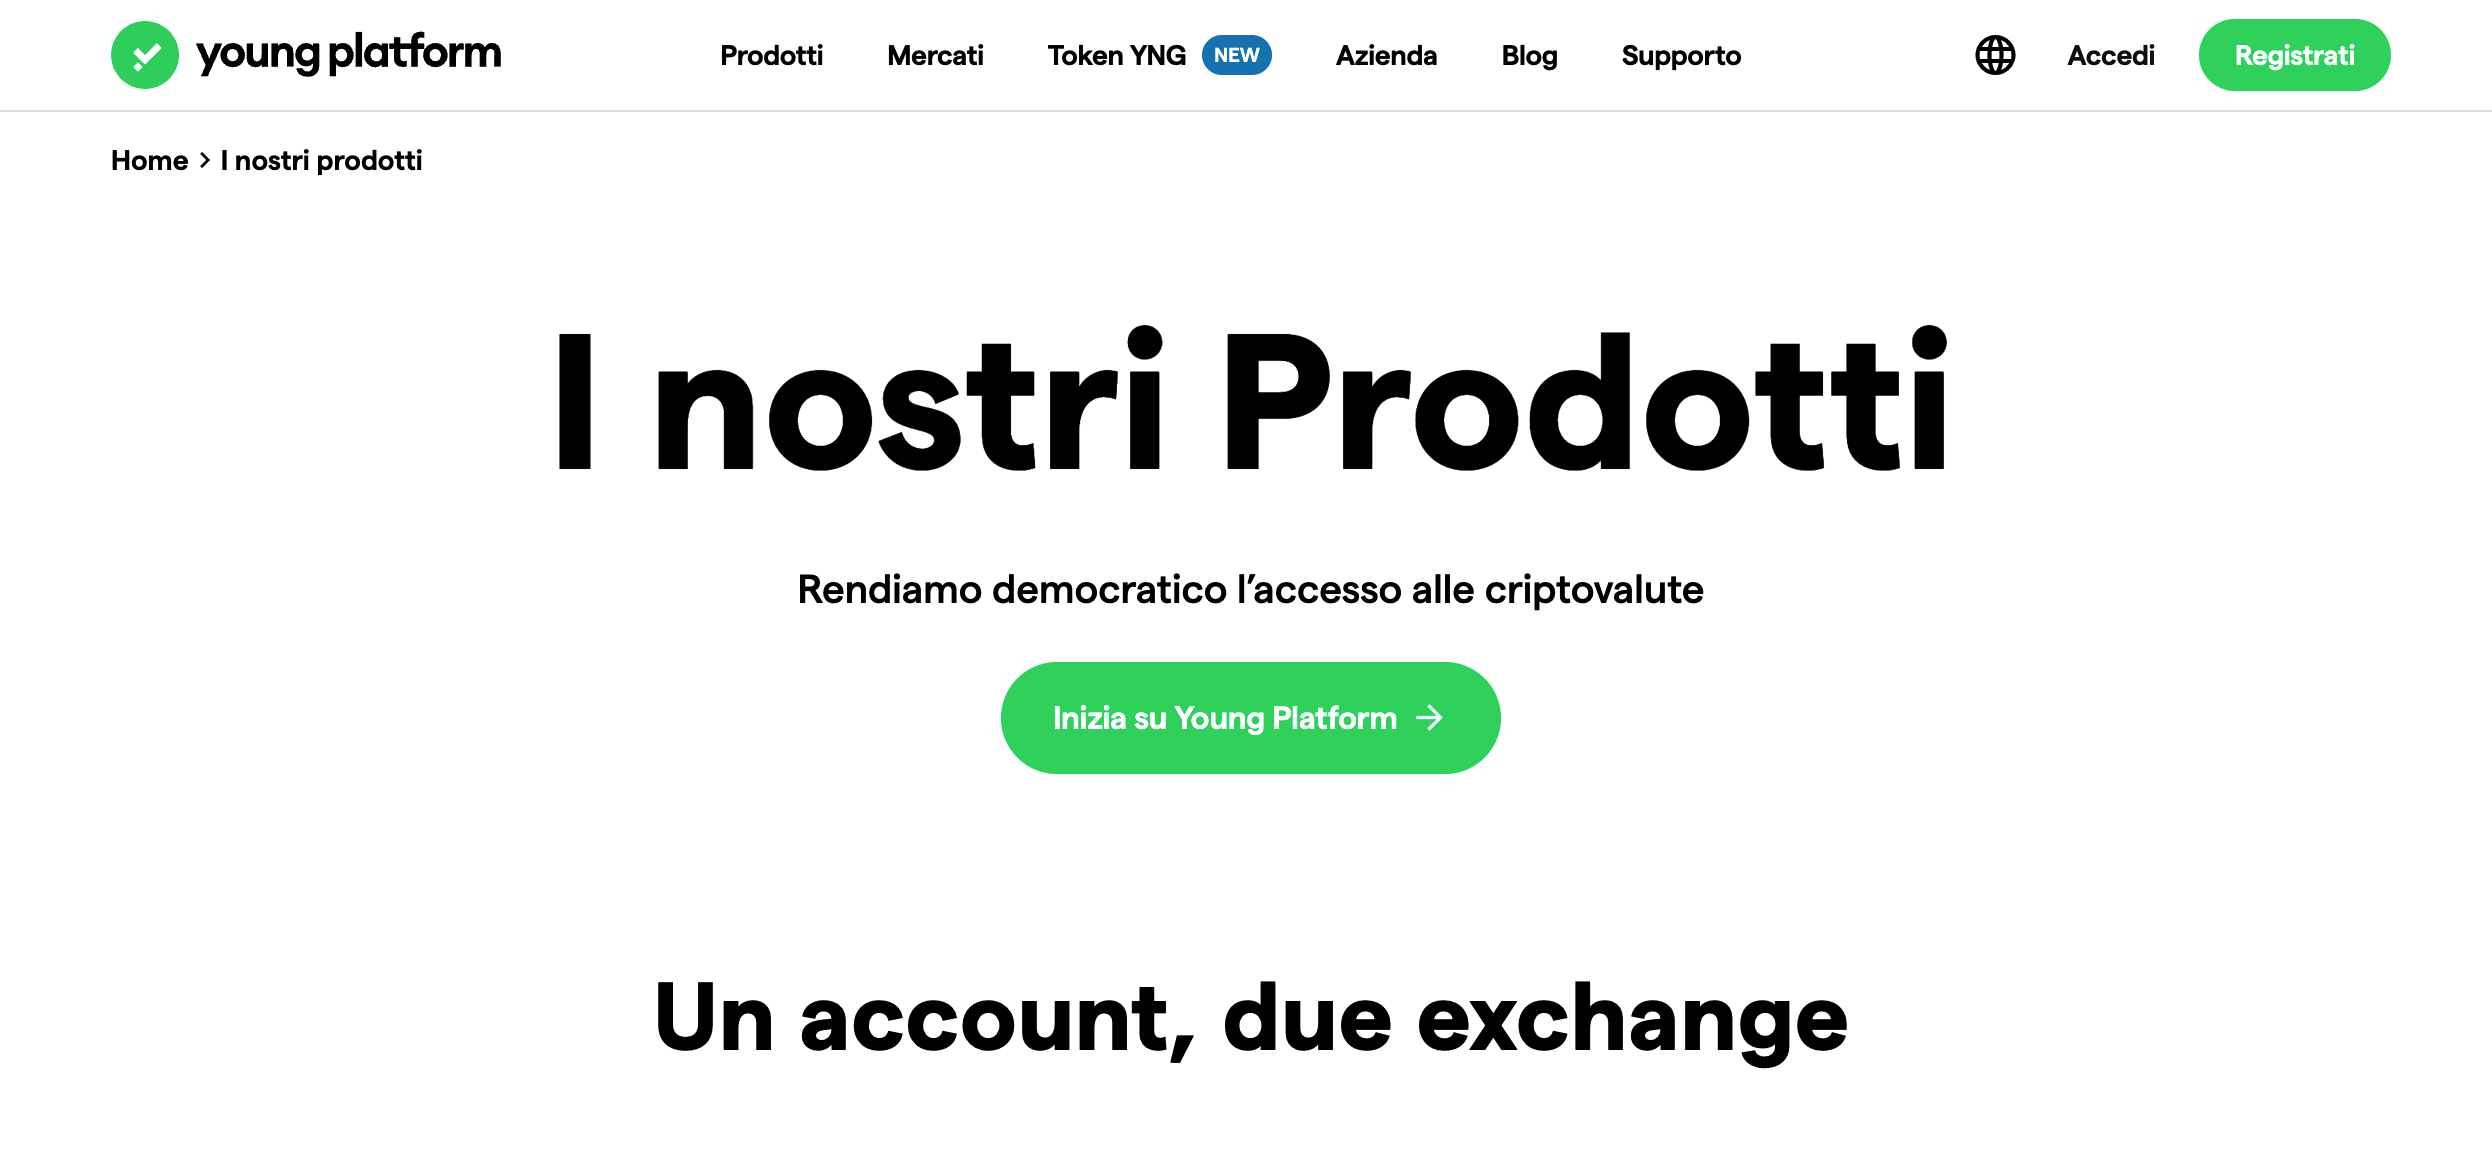
\includegraphics[width=0.70\textwidth]{res/images/internal-pages/products-page/products-page-1.png}
  \caption{Prima sezione della pagina dei prodotti.}
  \label{fig:products-page-1}
\end{figure}

\begin{figure}[H]
  \centering
  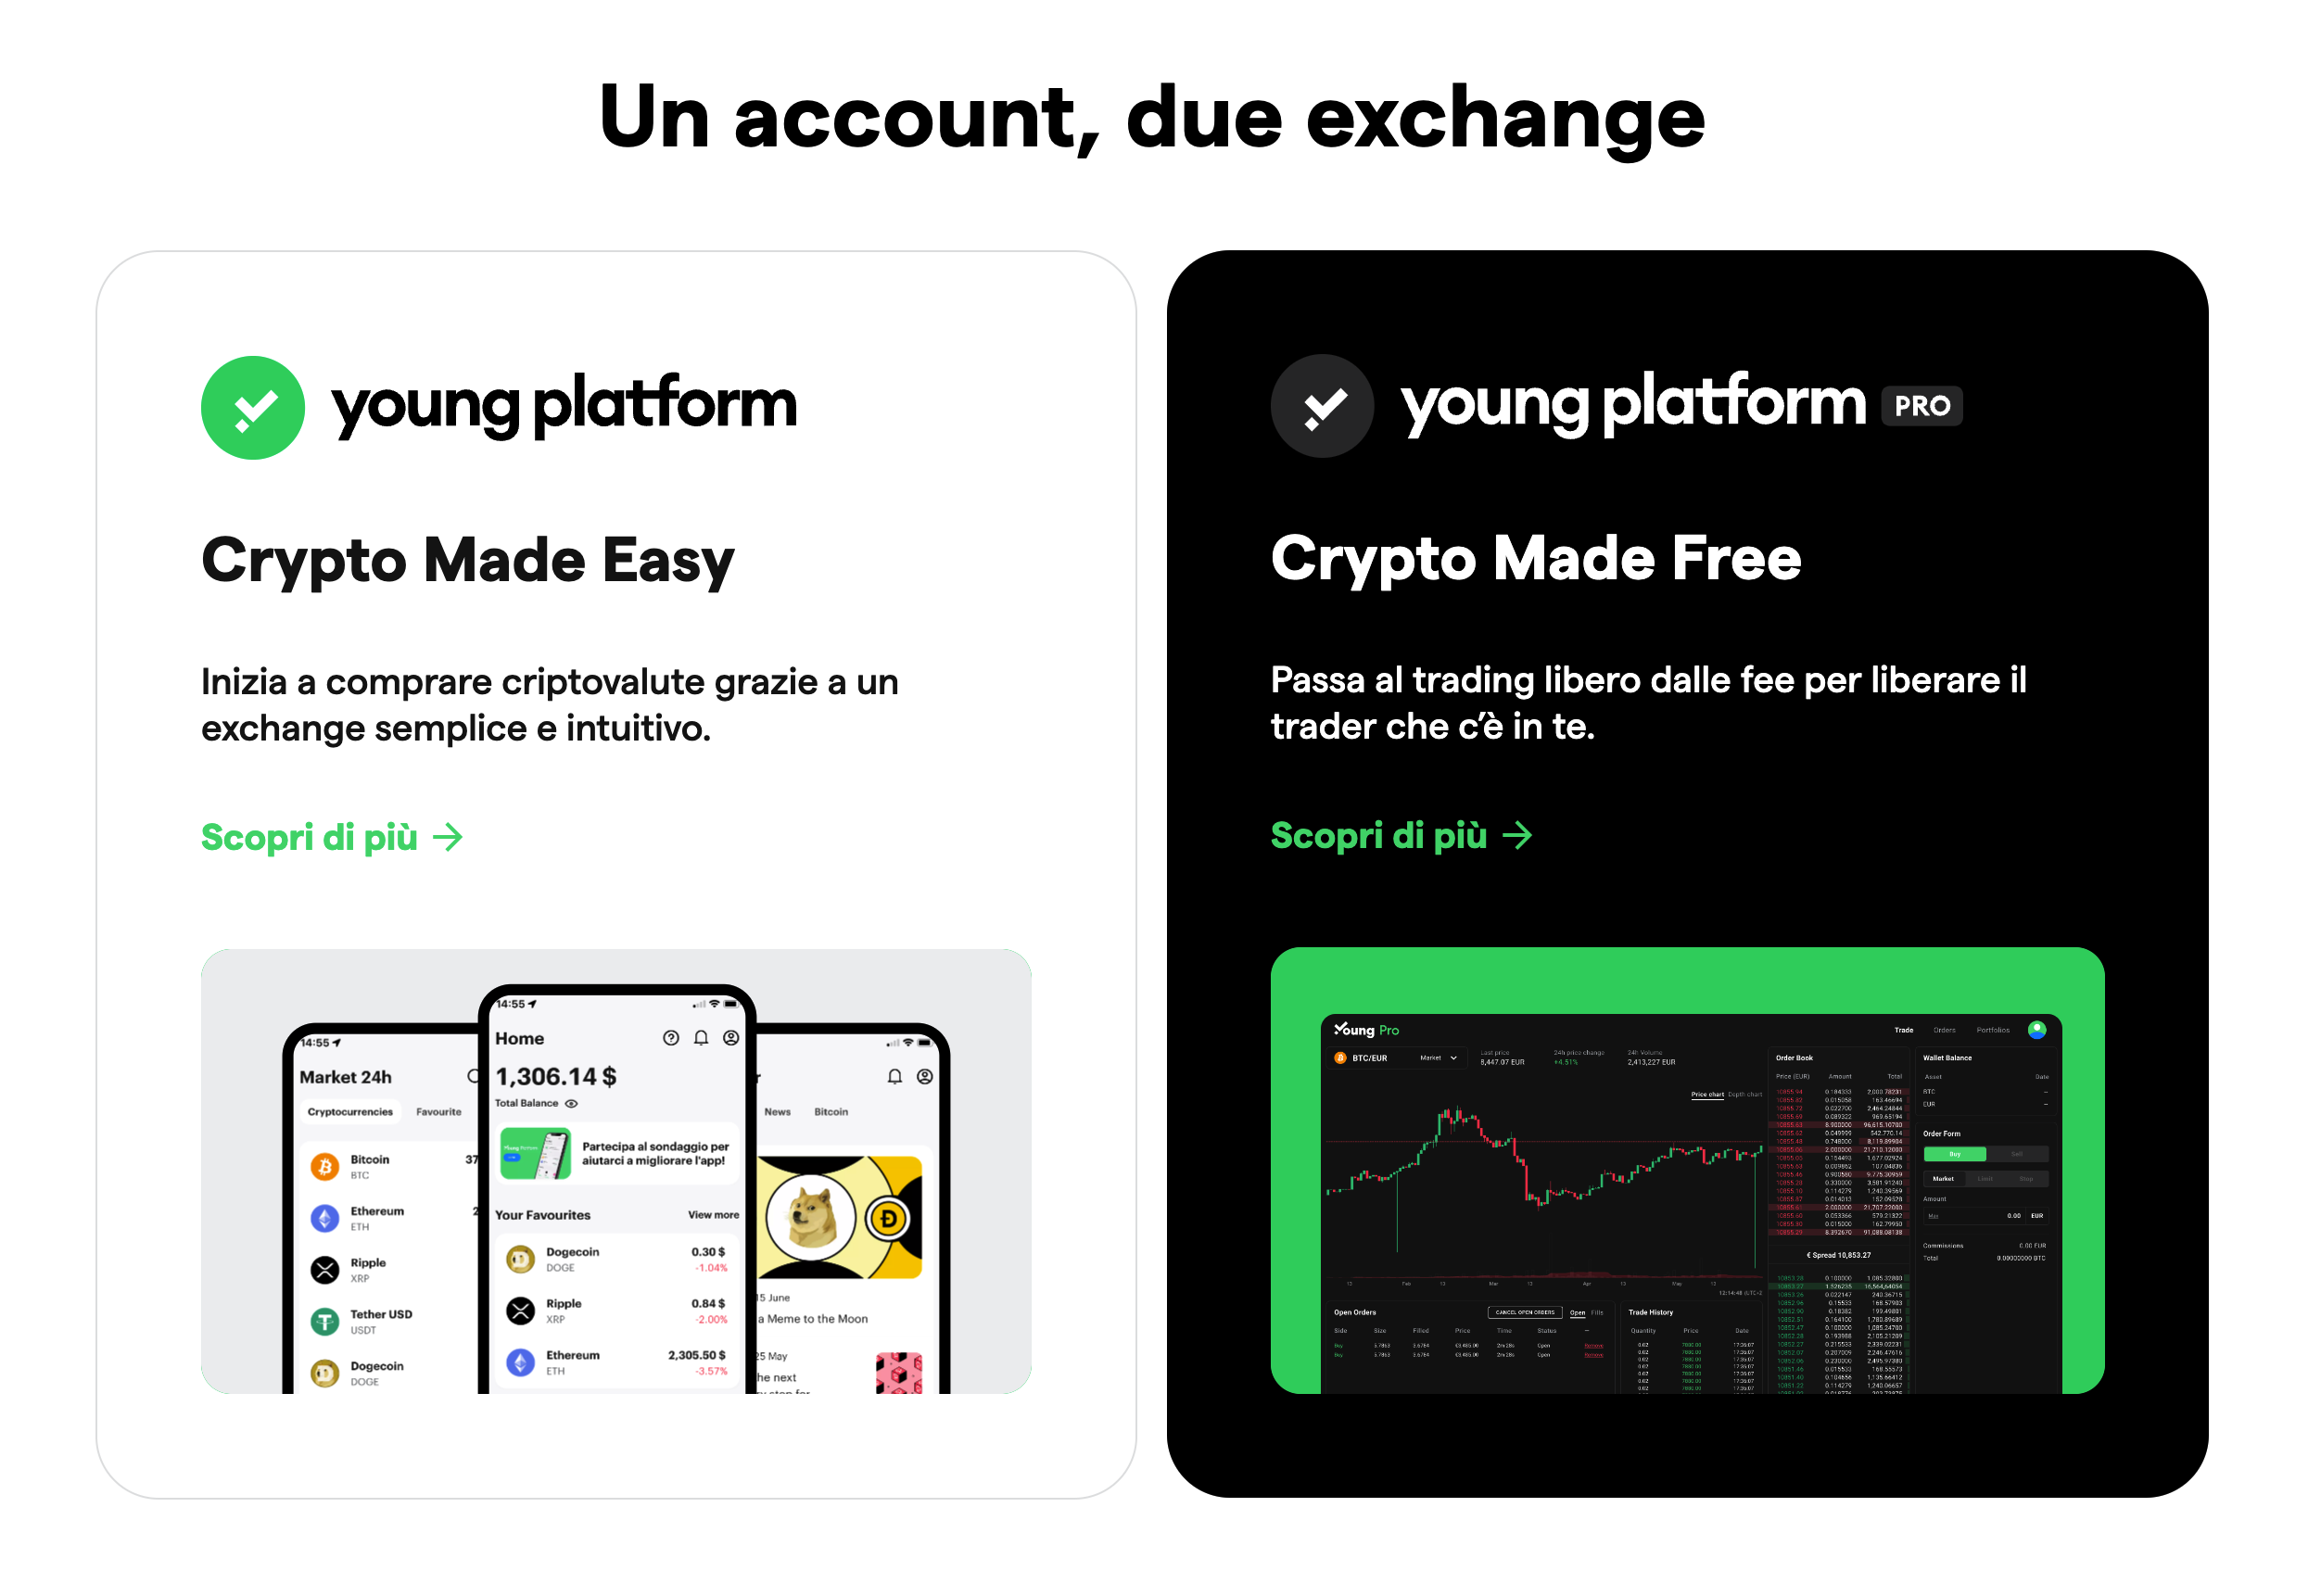
\includegraphics[width=0.80\textwidth]{res/images/internal-pages/products-page/products-page-2.png}
  \caption{Seconda sezione della pagina dei prodotti.}
  \label{fig:products-page-2}
\end{figure}

\begin{figure}[H]
  \centering
  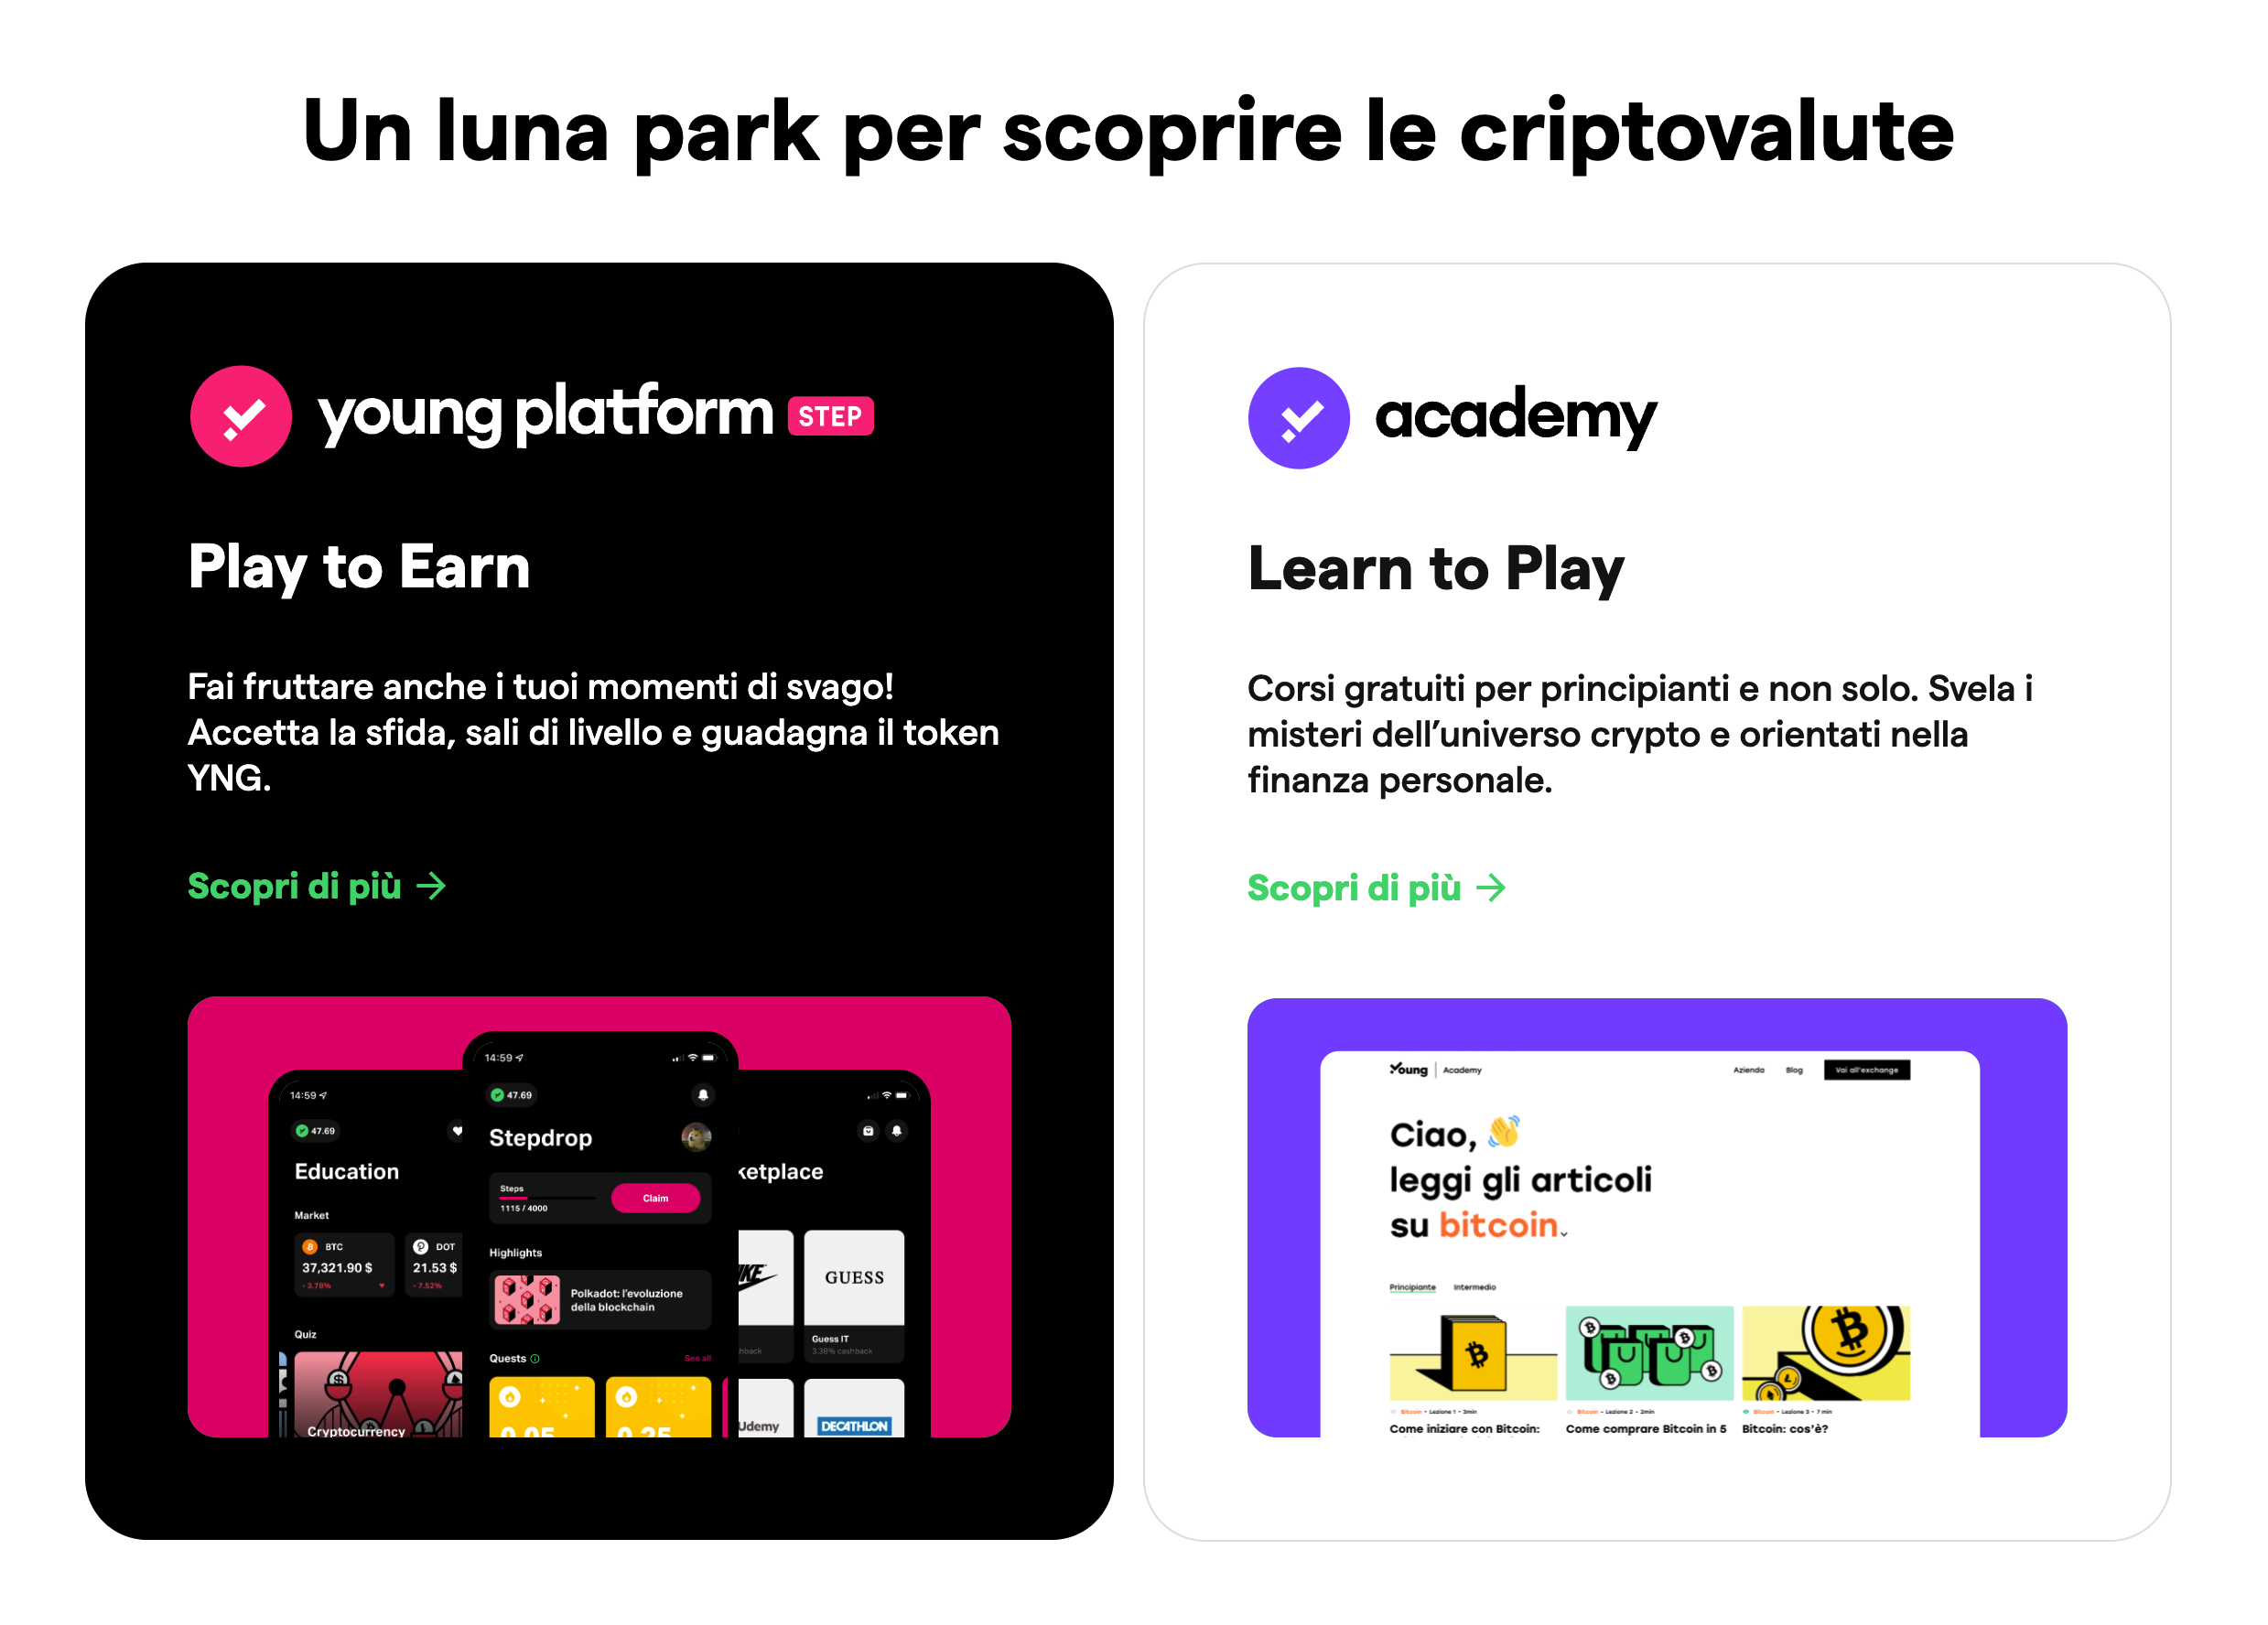
\includegraphics[width=0.80\textwidth]{res/images/internal-pages/products-page/products-page-3.png}
  \caption{Terza sezione della pagina dei prodotti.}
  \label{fig:products-page-3}
\end{figure}

\paragraph{Who}

Il logo aziendale è sempre presente in alto a sinistra, come illustrato 
nella figura \ref{fig:products-page-1}.

\paragraph{Where}

In questa pagina è presente un \textit{breadcrumb} e permette all'utente 
di non rimanere disorientato. L'utilizzo di questo elemento permette di 
comunicare in maniera efficace gran parte dell'asse where (in alto a 
sinistra, sotto al logo aziendale) (fig. \ref{fig:products-page-1}).

\paragraph{Why}

La pagina fornisce degli ottimi motivi per continuare ad esplorarla. 
Sopratutto per un utente principiante, questa pagina rappresenta una 
bussola per orientarsi per verso il mondo delle criptovalute e di 
esplorare i vari prodotti. 

\paragraph{When}

Questa pagina non informa alcun riferimento temporale. Pertanto, risulta 
difficile per l'utente capire se i prodotti illustrati sono aggiornati.

\paragraph{How}

Questa pagina è difficile da raggiungere in quanto per arrivare a questa 
pagina è necessario recarsi nel footer e cliccare alla voce 
\textit{I nostri prodotti} (quarta voce della terza colonna) 
(fig. \ref{fig:footer}). Questo rappresenta un grande svantaggio per 
l'utente.

\subsubsection{Academy page}

La pagina a cui si fa riferimento è raggiungibile al seguente indirizzo 
\href{https://academy.youngplatform.com/}{https://academy.youngplatform.com/}.

\paragraph{What}

L'obiettivo di questa pagina è ben comprensibile. Lo scopo di questa 
pagina è quello di offrire una serie di contenuti per educare e informare 
l'utente (fig. \ref{fig:academy-1} e \ref{fig:academy-2}). Gli articoli 
vengono raggruppati in macro-categorie (ad esempio la categoria 
\textit{Blockchain} in figura \ref{fig:academy-2}) e permette di guidare 
l'utente verso quali contenuti vuole fruire. 

\begin{figure}[H]
  \centering
  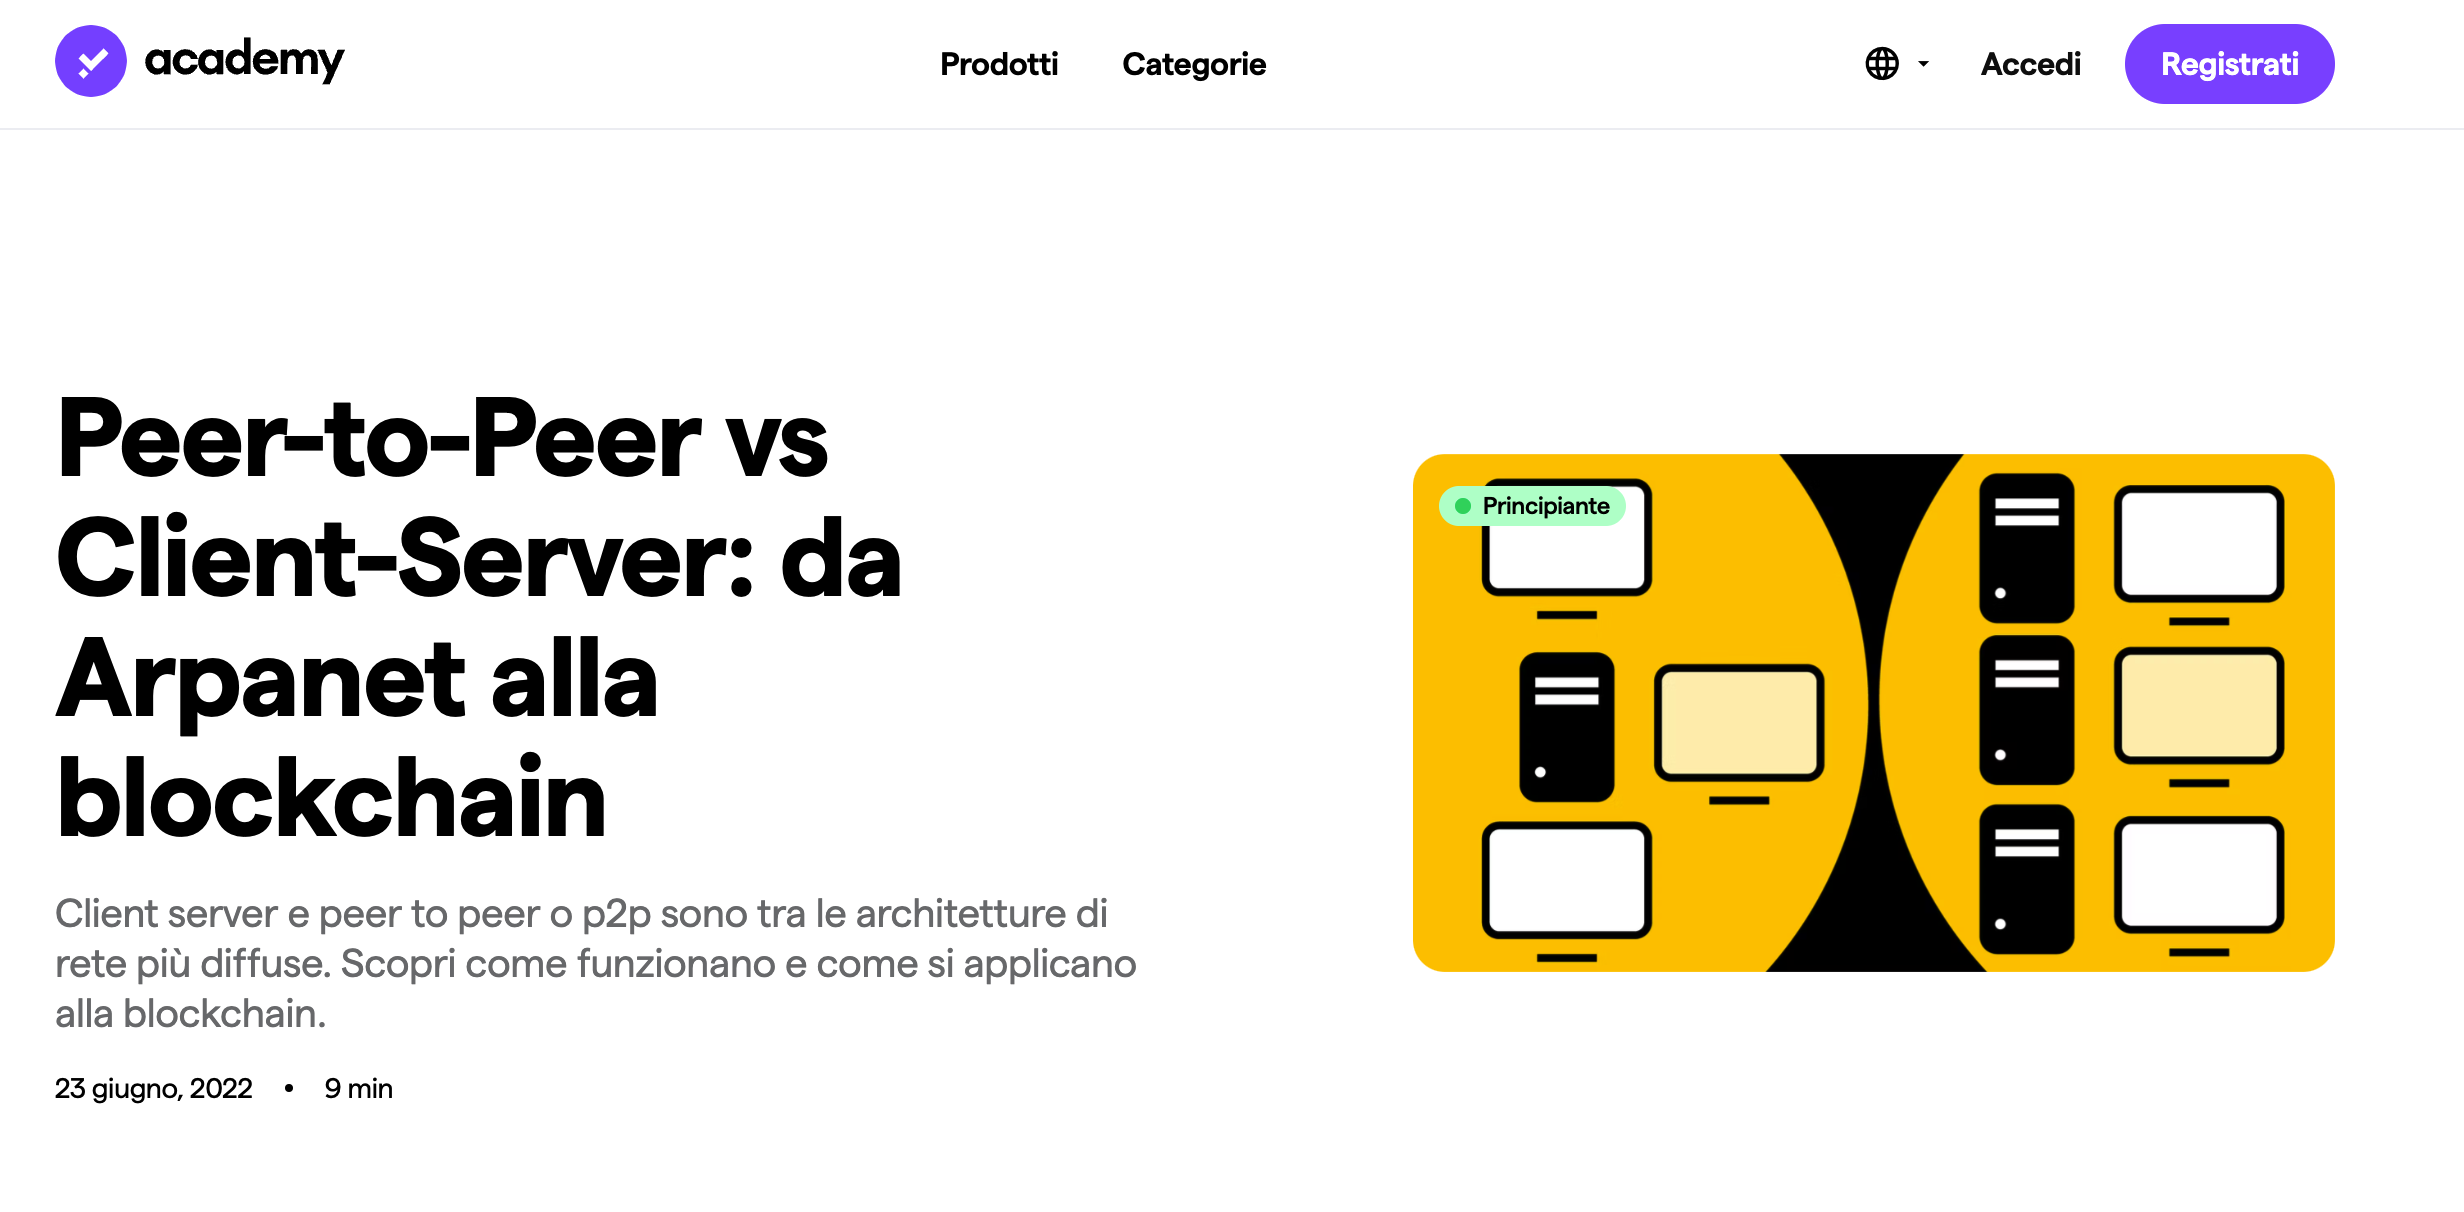
\includegraphics[width=0.80\textwidth]{res/images/internal-pages/academy/academy-1.png}
  \caption{Prima sezione della pagina \textit{Academy}.}
  \label{fig:academy-1}
\end{figure}

\begin{figure}[H]
  \centering
  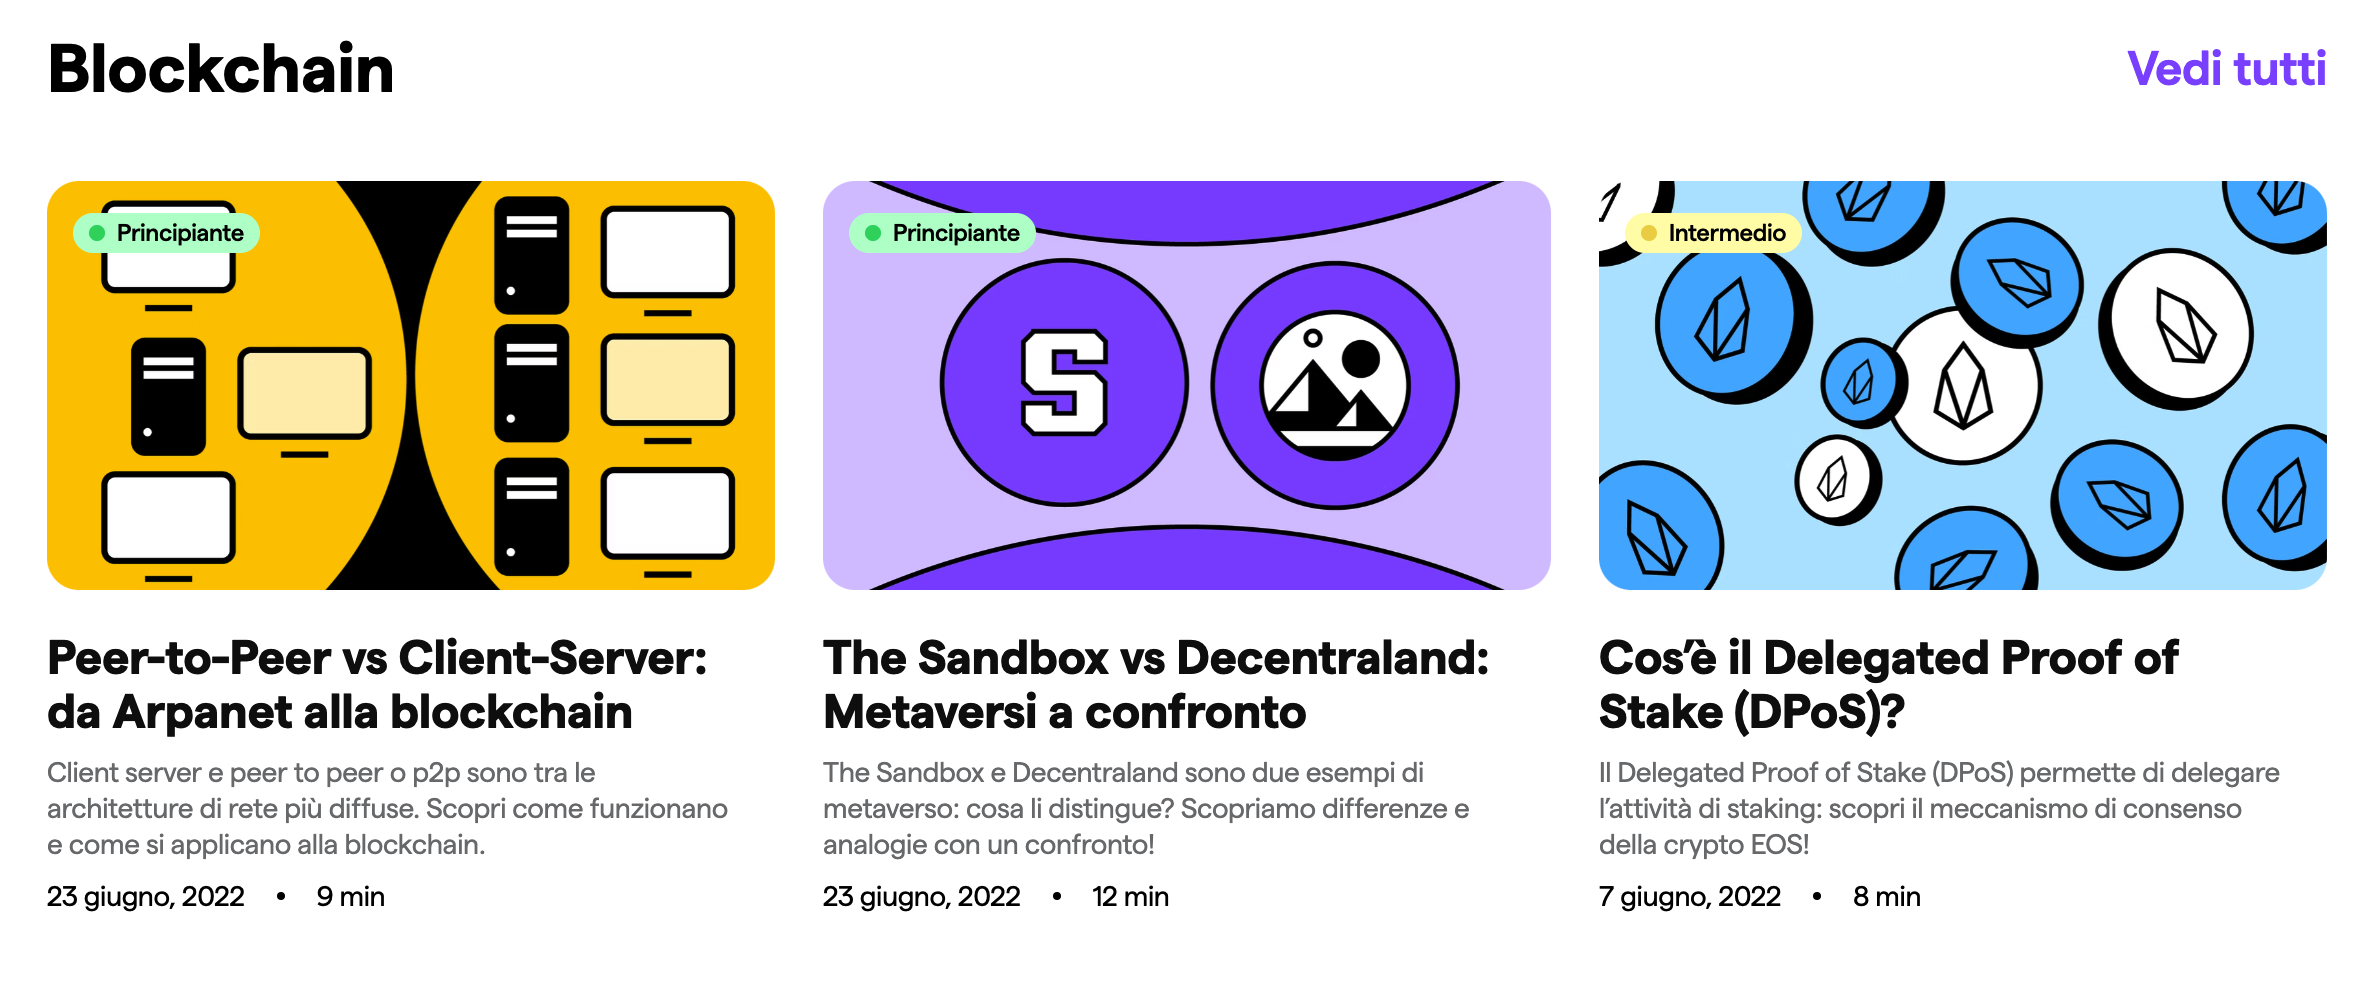
\includegraphics[width=0.80\textwidth]{res/images/internal-pages/academy/academy-2.png}
  \caption{Prima categoria della pagina \textit{Academy}.}
  \label{fig:academy-2}
\end{figure}

\paragraph{Who}

Il logo aziendale è presente in alto a sinistra, come illustrato 
nella figura \ref{fig:academy-1}. Tuttavia, ha un colore diverso rispetto 
al colore originale (verde). L'azienda ha scelto di colorare il logo con 
un colore diverso per ogni prodotto. L'utente riesce comunque a riconoscere 
il logo in sè, anche se non è del colore originale. 

\paragraph{Where}

Quando l'utente viene reindirizzato a questa pagina, si può notare che si 
è arrivati in un nuovo sottodominio (\textit{academy.youngplatform.com}). 
Non è presente però un elemento che permette di ritornare alla pagina a cui 
si è arrivati o per ritornare alla homepage di \textit{youngplatform.com}. 
Per poter tornare alla homepage è necessario recarsi nel footer. Questa 
implementazione è molto svanataggiosa per l'utente e richiede dello sforzo 
per compiere l'azione.

\paragraph{Why}

Questa pagina offre degli ottimi motivi per esplorarla:
\begin{itemize}
  \item Per gli utenti principianti è possibile attingere a una gran 
  quantità di articoli che permettono di introdurre al mondo delle 
  criptovalute e della blockchain;
  \item Per gli utenti esperti è possibile comunque leggere degli articoli 
  che riguardano le ultime novità del settore o degli articoli che 
  illustrano dei confronti tra due tecnologie/competitor.
\end{itemize}

Inoltre, è possibile notare che l'elemento che rappresenta l'articolo è 
composto da un'immagine, da un titolo, da una breve descrizione di 
introduzione e da riferimenti temporali. Posto in alto a sinistra 
dell'immagine è presente un elemento che indica a chi è rivolto questo 
articolo, ovvero, gli articoli vengono suddivisi tra \textit{Principiante}, 
\textit{Intermedio} ed \textit{Esperto}. Questa strategia è molto utile 
in quanto permette ad un utente di scegliere gli articoli che coincidono 
con la propria esperienza nel settore.

\paragraph{When}

In questa pagina ci sono dei chiari riferimenti temporali: è possibile 
notare che per ogni articolo presente nella pagina è presente la data di 
pubblicazione dell'articolo (fig. \ref{fig:academy-1} e 
\ref{fig:academy-2}). Inoltre, come illustrato nella figura 
\ref{fig:academy-1}, nella sezione iniziale di questa pagina viene posto 
l'ultimo articolo pubblicato, mettendolo in evidenza. 

\paragraph{How}

Questa pagina è facile da raggiungere, in quanto è sufficiente 
recarsi nel menù principale di \textit{youngplatform.com} alla voce 
\textit{Prodotti}. Questa pagina può essere raggiunta anche tramite il 
footer.

\subsubsection{Academy - Blockchain}

La pagina a cui si fa riferimento è raggiungibile al seguente indirizzo \\
\href{https://academy.youngplatform.com/blockchain/}{https://academy.youngplatform.com/blockchain/}. 

\paragraph{What}

Questa pagina dichiara esplicitamente che cosa viene offerto, ovvero, 
vengono offerti una serie di articoli che trattano l'argomento 
\textit{Blockchain}. 

\begin{figure}[H]
  \centering
  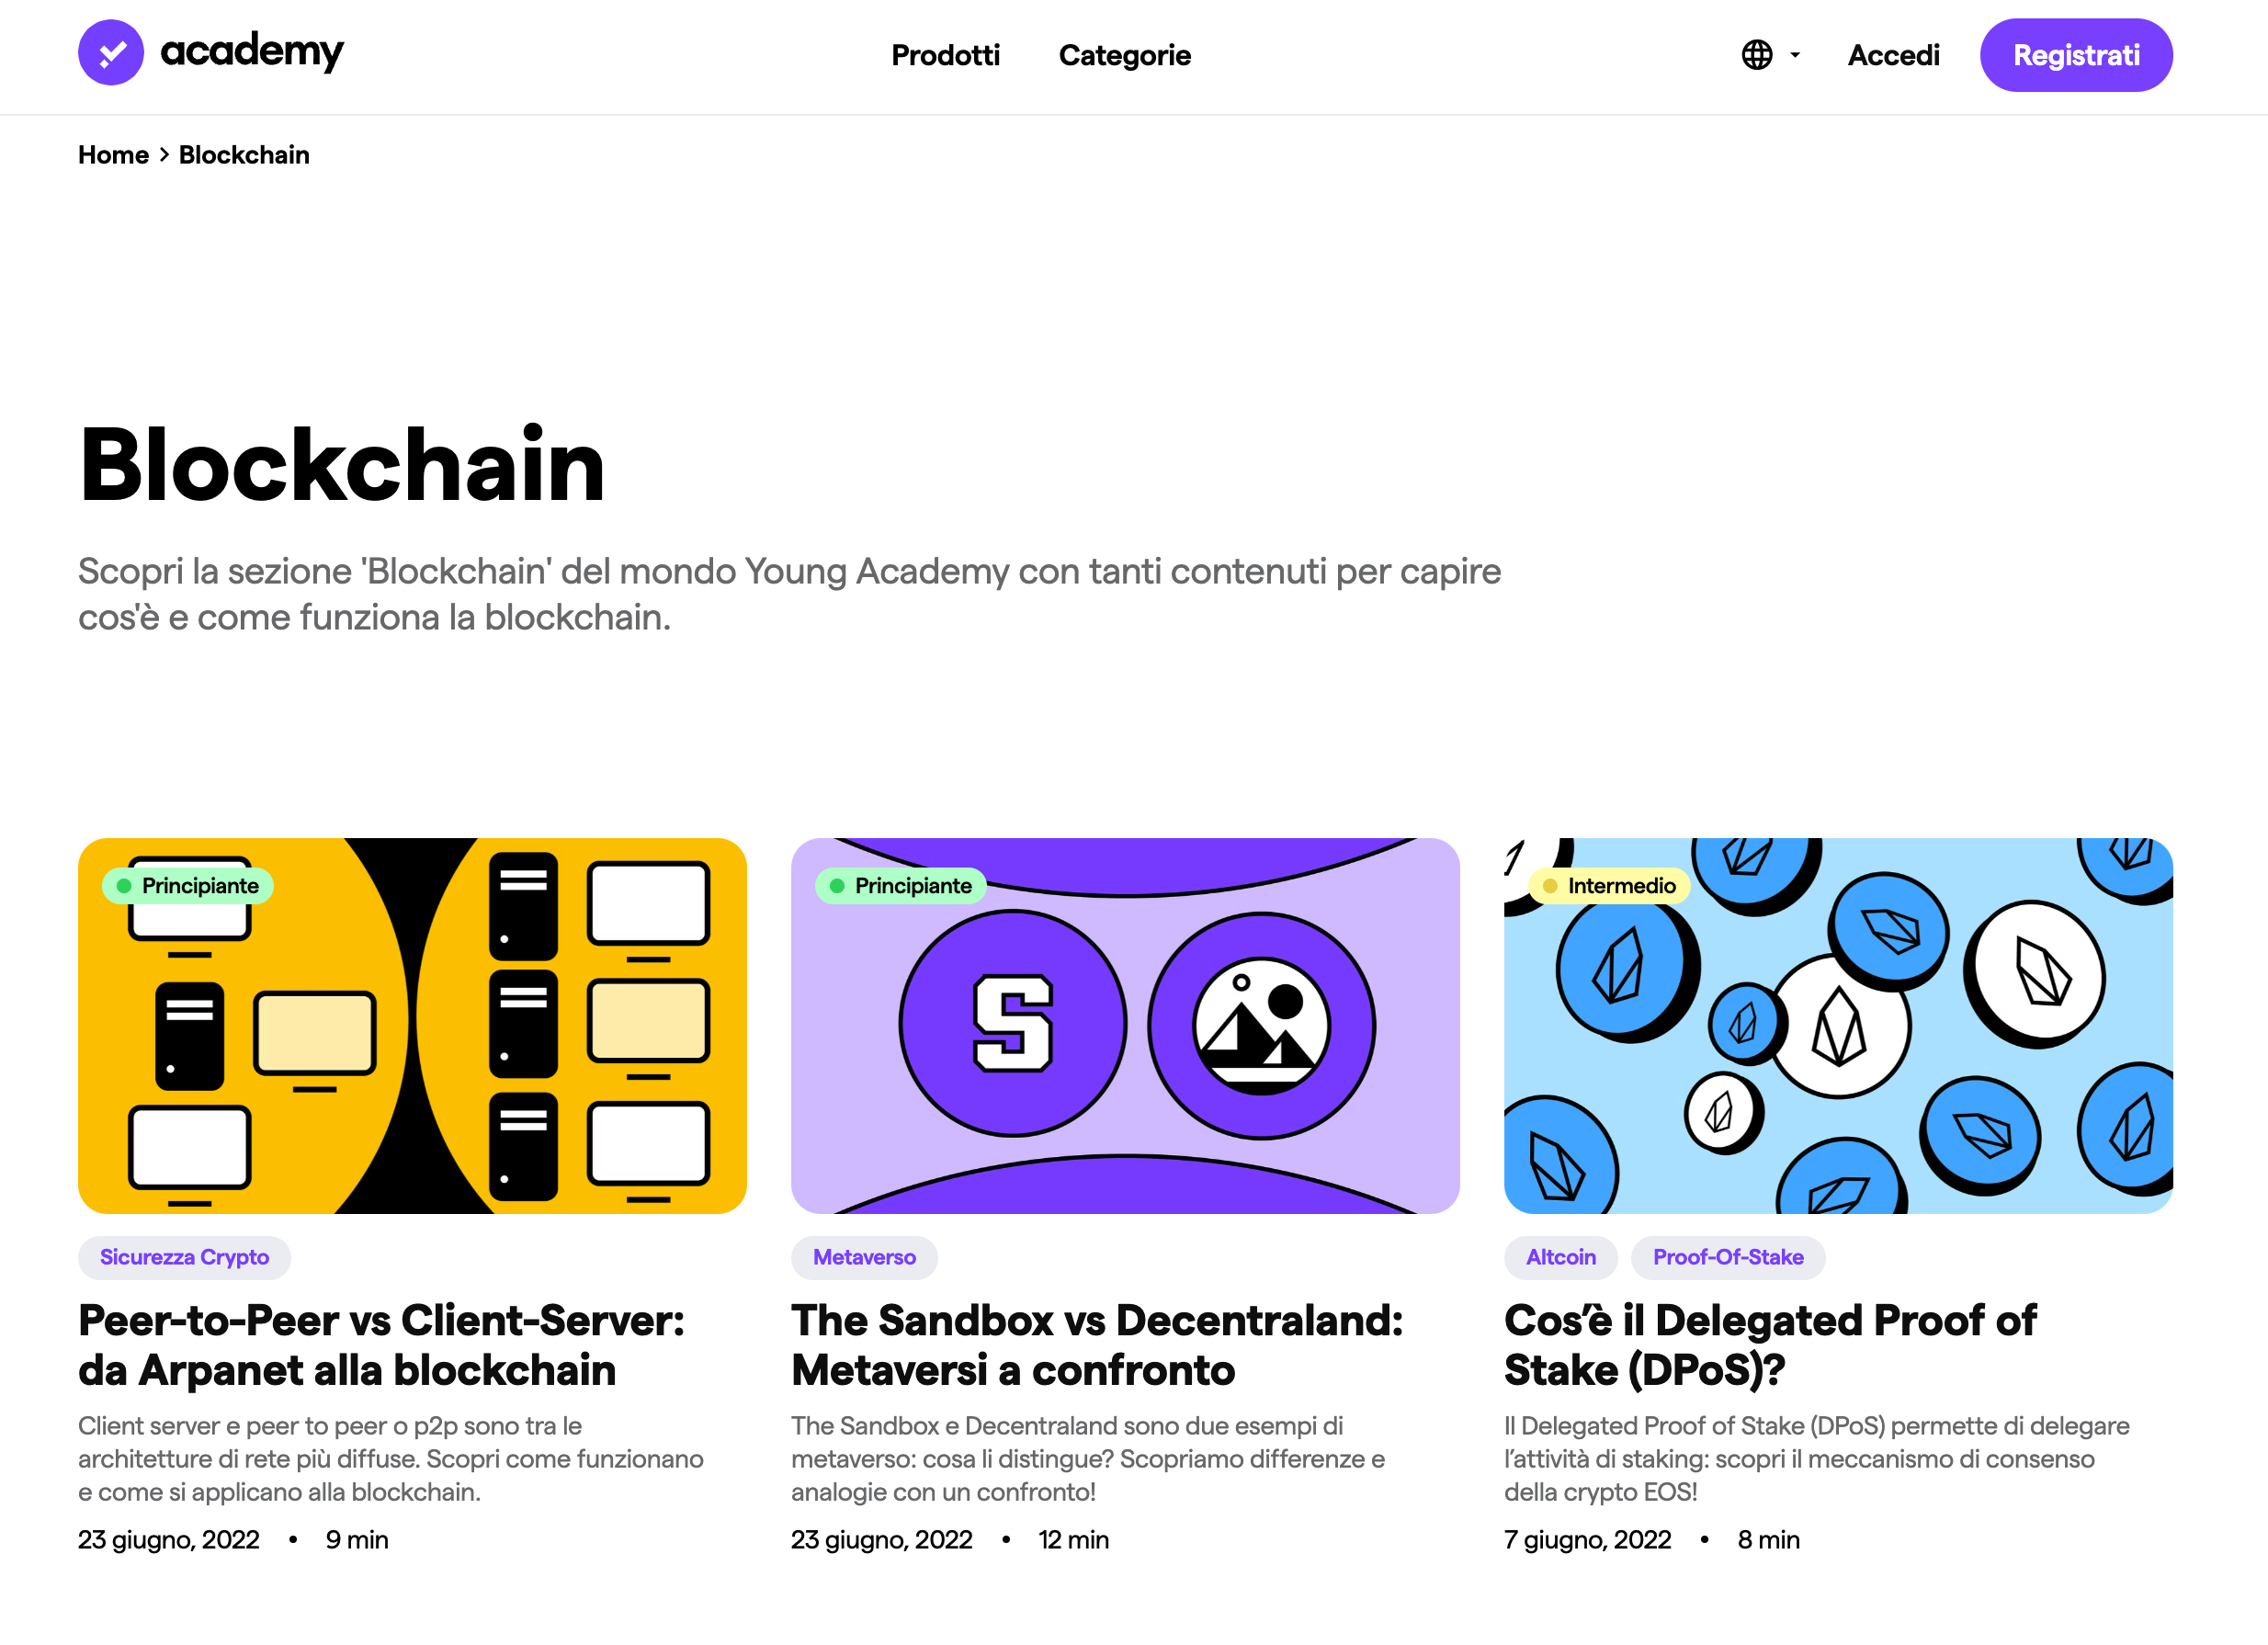
\includegraphics[width=0.80\textwidth]{res/images/internal-pages/academy/academy-3.png}
  \caption{Sezione di articoli della categoria \textit{Blockchain}.}
  \label{fig:academy-3}
\end{figure}

\paragraph{Who}

Il logo aziendale è presente in alto a sinistra, come illustrato 
nella figura \ref{fig:academy-3}.

\paragraph{Where}

In questa pagina è presente un \textit{breadcrumb} e permette all'utente 
di non rimanere disorientato. L'utilizzo di questo elemento permette di 
comunicare in maniera efficace gran parte dell'asse where (in alto a 
sinistra, sotto al logo aziendale) (fig. \ref{fig:academy-3}). È possibile 
notare inoltre che a fine pagina nella figura \ref{fig:academy-4} 
(in basso a destra) è presente un elemento \textit{Precedenti}. Questo 
elemento comunica all'utente che i contenuti sono \textit{paginati}, 
ovvero, ogni pagina presenta un certo numero di articoli. Se si vuole 
cercare un articolo più vecchio, il sito offre un modo per navigare e 
ricercare altri articoli.

\begin{figure}[H]
  \centering
  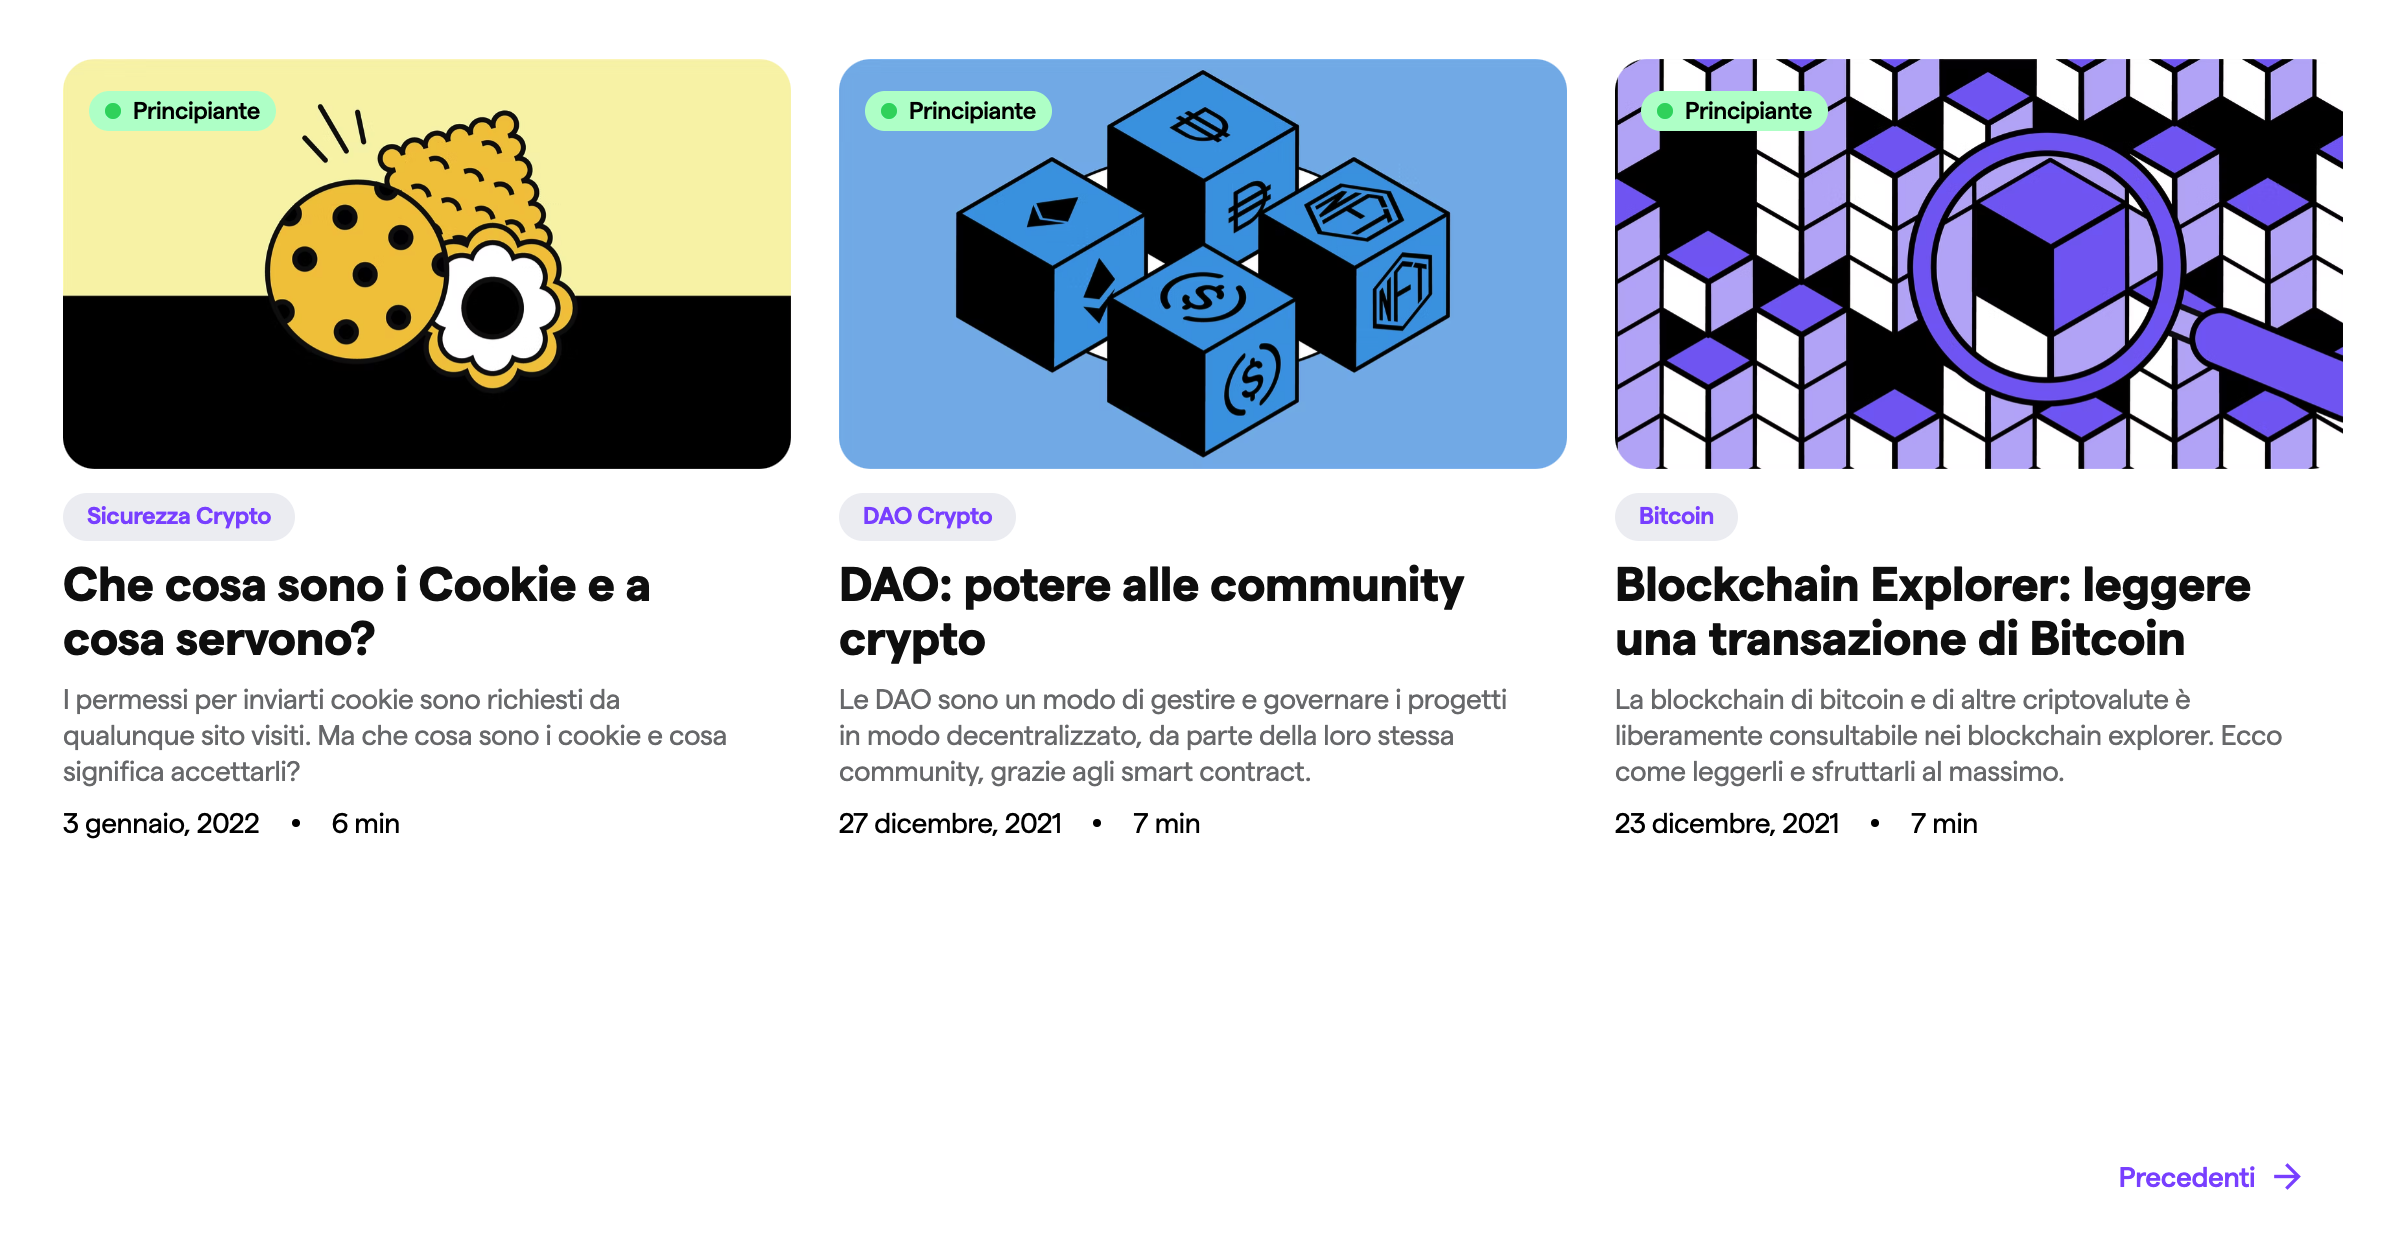
\includegraphics[width=0.80\textwidth]{res/images/internal-pages/academy/academy-4.png}
  \caption{Fine pagina della categoria \textit{Blockchain}.}
  \label{fig:academy-4}
\end{figure}

\paragraph{Why}

Questa pagina offre dei motivi differenti per continuare ad esplorarla. 
Se l'utente è inesperto del settore, allora l'utente vorrà leggere 
diversi articoli e esplorare la pagina per ricercare dei contenuti 
introduttivi. Se l'utente è esperto, l'utente esplorerà la pagina per 
ricercare un articolo specifico, in modo da ottenere direttamente 
l'informazione ricercata.

\paragraph{When}

In questa pagina ci sono presenti dei riferimenti temporali: è possibile 
notare che per ogni articolo presente nella pagina è presente la data di 
pubblicazione dell'articolo (fig. \ref{fig:academy-3}).

\paragraph{How}

Questa pagina non è facile da raggiungere in quanto rappresenta una 
categoria di articoli specifica. Pertanto, se l'utente necessita delle 
informazioni che riguardano questo argomento, dovrà effettuare una ricerca. 
In questo caso particolare, questa pagina è possibile raggiungerla dalla 
pagina 
\href{https://academy.youngplatform.com/}{https://academy.youngplatform.com/}, 
cliccando alla voce \textit{Vedi tutti} (posto in alto a destra, di colore 
viola).

\subsubsection{Academy - Blockchain - Article}

La pagina a cui si fa riferimento è raggiungibile al seguente indirizzo \\
\href{https://academy.youngplatform.com/blockchain/peer-to-peer-p2p-client-server-cosa-sono-come-funzionano/}{https://academy.youngplatform.com/blockchain/peer-to-peer-p2p-client-server-cosa-sono-come-funzionano/}.

\paragraph{What}

Questa pagina dichiara esplicitamente il contenuto che viene offerto 
all'utente, in particolare, in tale pagina, verrà offerto un contenuto 
molto specifico che è stato scelto dall'utente. 

\begin{figure}[H]
  \centering
  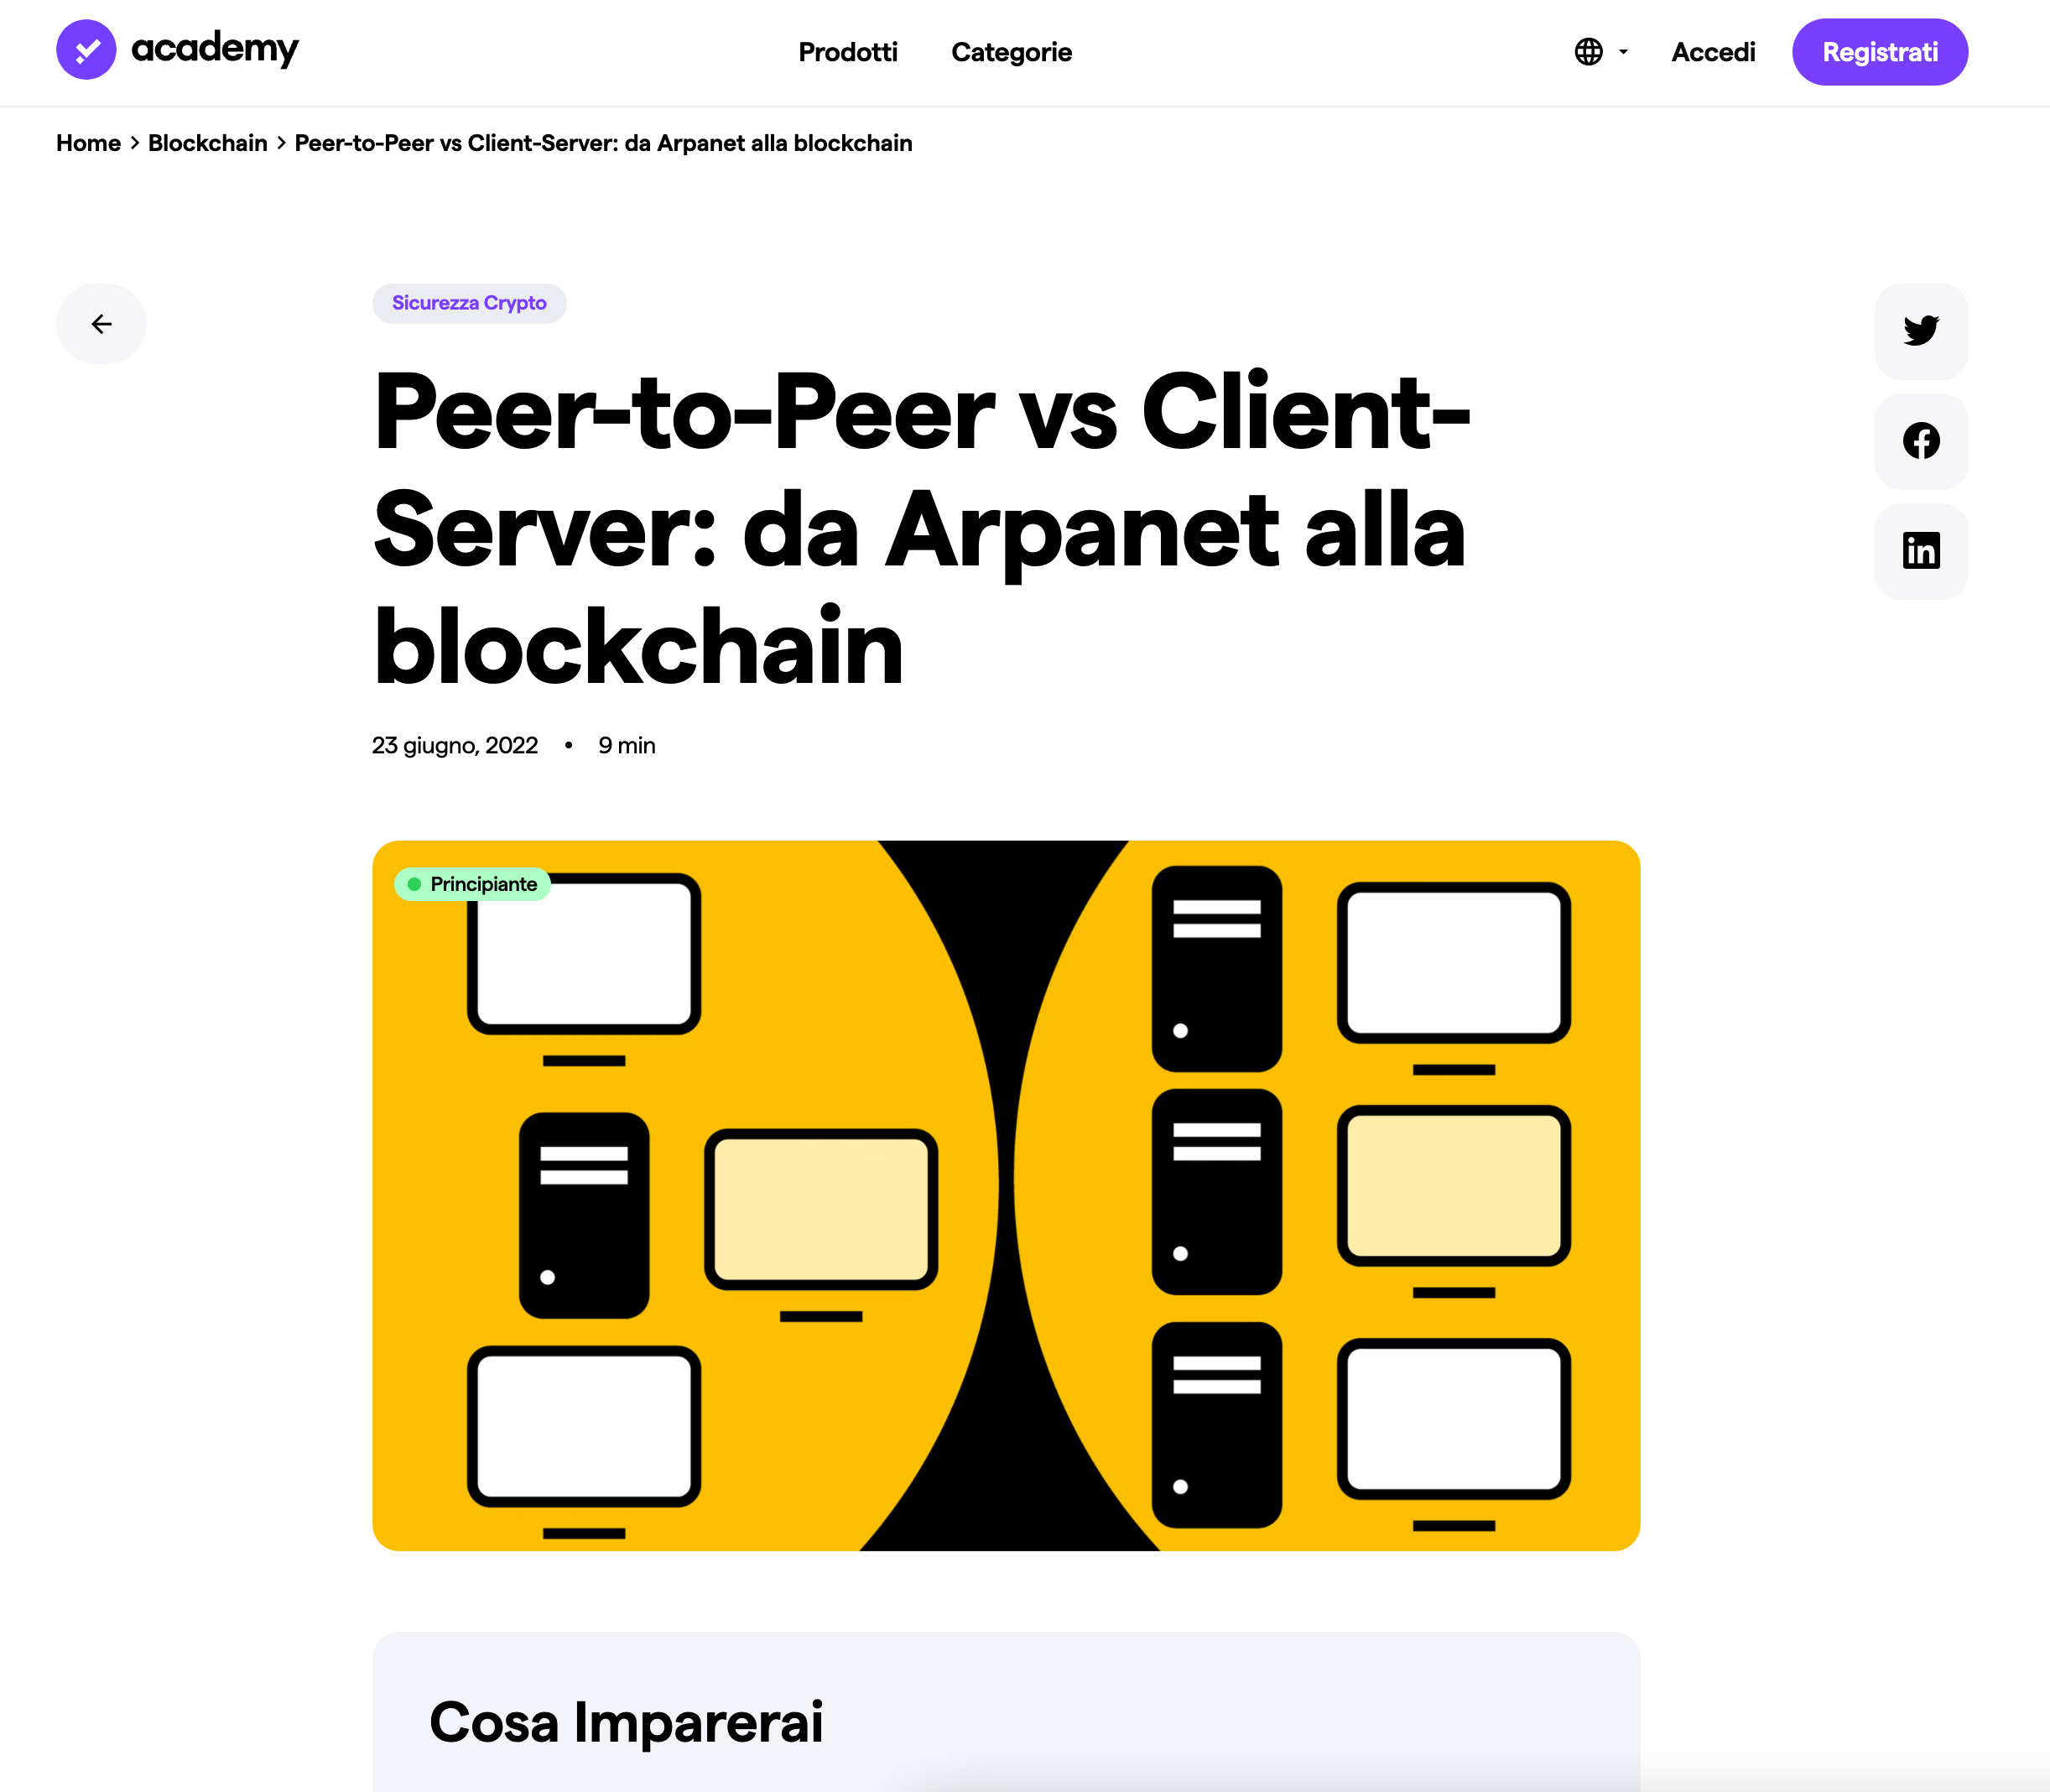
\includegraphics[width=0.80\textwidth]{res/images/internal-pages/academy/academy-5.png}
  \caption{Un articolo della categoria \textit{Blockchain}.}
  \label{fig:academy-5}
\end{figure}

\paragraph{Who}

Il logo aziendale è presente in alto a sinistra, come illustrato 
nella figura \ref{fig:academy-5}.

\paragraph{Where}

Anche in questa pagina è presente un \textit{breadcrumb} e permette 
all'utente di non rimanere disorientato. L'utilizzo di questo elemento 
permette di comunicare in maniera efficace gran parte dell'asse where 
(in alto a sinistra, sotto al logo aziendale) (fig. \ref{fig:academy-5}). 
È possibile notare inoltre che in figura \ref{fig:academy-6}, sotto al 
logo aziendale, è presente una barra di colore viola. Tale barra indica 
a che punto è l'utente nella lettura dell'articolo. Quindi, in particolare, 
la lunghezza della barra viola indica la porzione di testo che è stato 
letto. Questo elemento è molto utile per l'utente in quanto può 
rendersi effettivamente conto della lunghezza dell'articolo.

\begin{figure}[H]
  \centering
  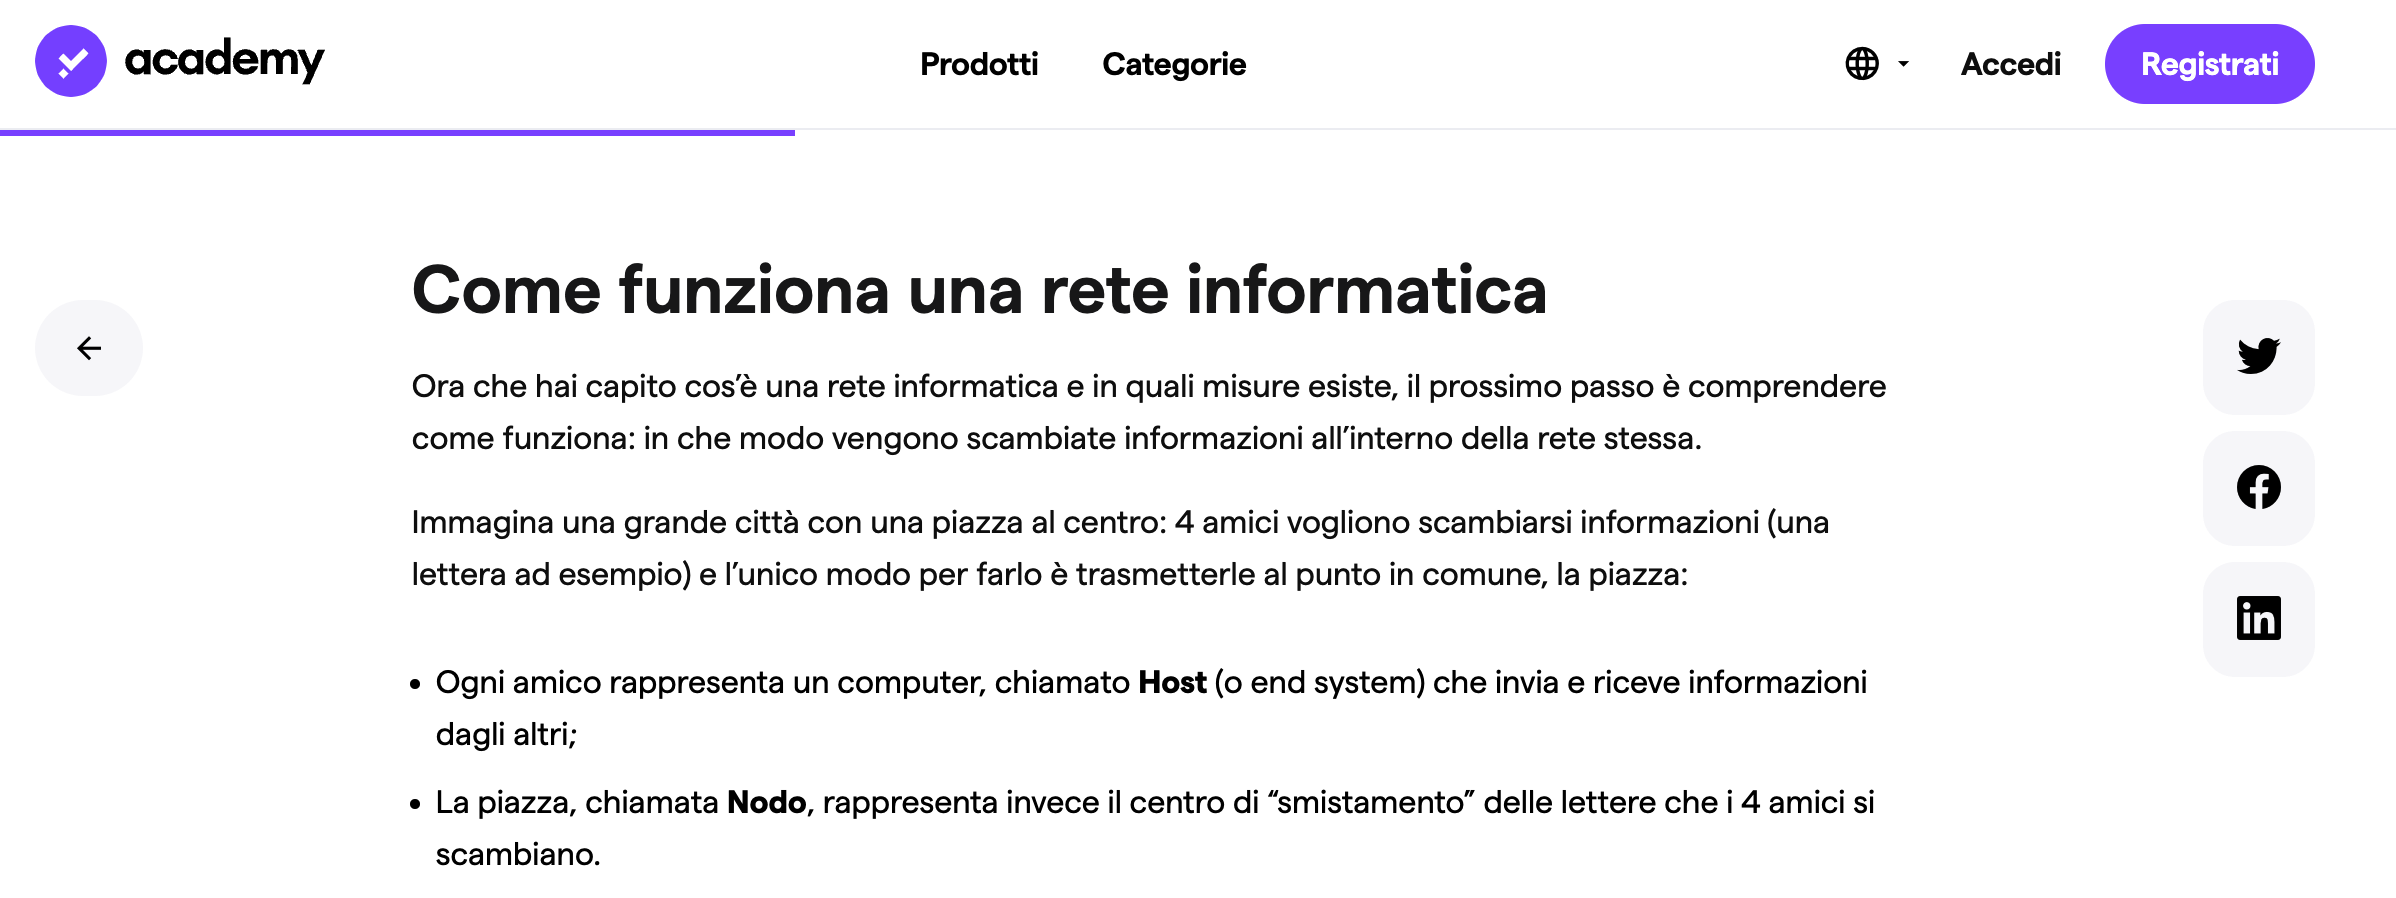
\includegraphics[width=0.80\textwidth]{res/images/internal-pages/academy/academy-6.png}
  \caption{Barra dinamica che indica a che punto si è arrivati con la 
  lettura dell'articolo.}
  \label{fig:academy-6}
\end{figure}

C'è un altro elemento nella pagina che aumenta l'usabilità del sito: 
in figura \ref{fig:academy-5} a sinistra c'è una freccia che permette di 
tornare indietro, nella lista di articoli della categoria 
\textit{Blockchain}. Tale elemento rimane sempre nella stessa posizione 
anche se l'utente scorre la pagina (si veda anche figura 
\ref{fig:academy-6}). Questo è un aspetto postivo perchè se l'utente vuole 
tornare alla pagina precedente, non è necessario che l'utente ritorni ad 
inizio pagina.

\paragraph{Why}

Il motivo principale per cui l'utente dovrebbe esplorare la pagine è che 
è direttamente interessato a questo articolo. A fine pagina, il sito 
propone, in una apposita sezione, degli ulteriori articoli correlati a 
quello appena letto (fig. \ref{fig:academy-7}). Questo fornisce un 
ulteriore motivo per continuare ad esplorare il sito.

\begin{figure}[H]
  \centering
  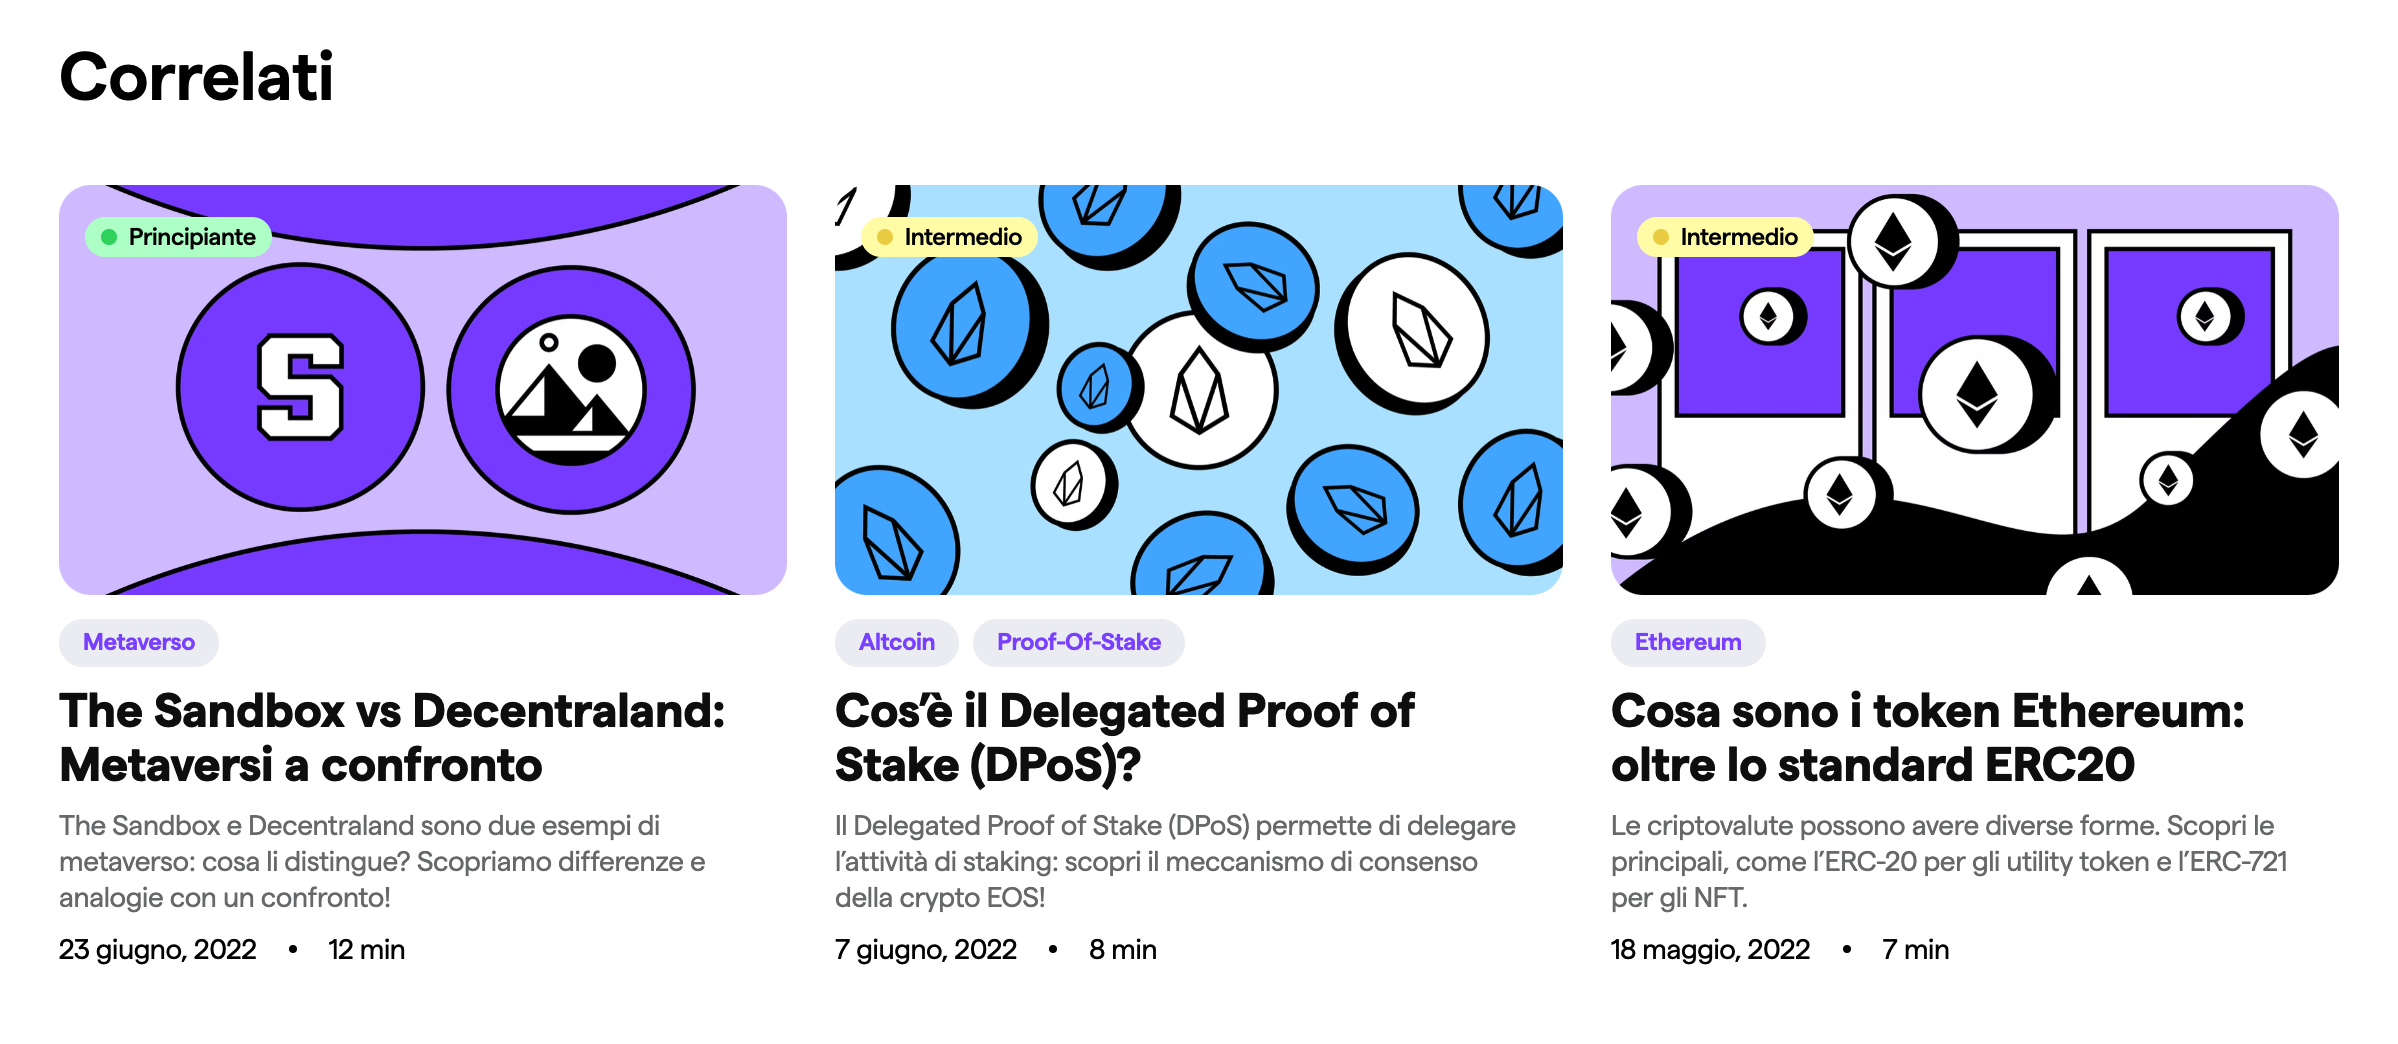
\includegraphics[width=0.80\textwidth]{res/images/internal-pages/academy/academy-7.png}
  \caption{Fine pagina dell'articolo.}
  \label{fig:academy-7}
\end{figure}

\paragraph{When}

In questa pagina è presente un riferimento temporale ed è possibile 
localizzarlo sotto al titolo dell'articolo (fig. \ref{fig:academy-5}).

\paragraph{How}

Questa pagina non è facile da raggiungere, in quanto l'utente deve 
essere effettivamente interessato a tale articolo. Pertanto, l'utente 
dovrà effettuare una ricerca per trovare tale articolo. Purtroppo la 
ricerca deve essere effettuata tramite un motore di ricerca, oppure, 
l'utente dovrebbe esplorare la pagine precedente per trovare l'articolo.
Questa pagina è possibile raggiungerla tramite 
\href{https://academy.youngplatform.com/blockchain/}{https://academy.youngplatform.com/blockchain/}.

\subsubsection{Glossary page}

La pagina a cui si fa riferimento è raggiungibile al seguente indirizzo 
\href{https://youngplatform.com/glossary/}{https://youngplatform.com/glossary/}.

\paragraph{What}

Il contenuto di questa pagina è dichiarato esplicitamente, ovvero, 
l'obiettivo di questa pagina è quella di racchiudere un insieme di termini 
tecnici del settore e di fornire una descrizione per ognuno di essi. 

\begin{figure}[H]
  \centering
  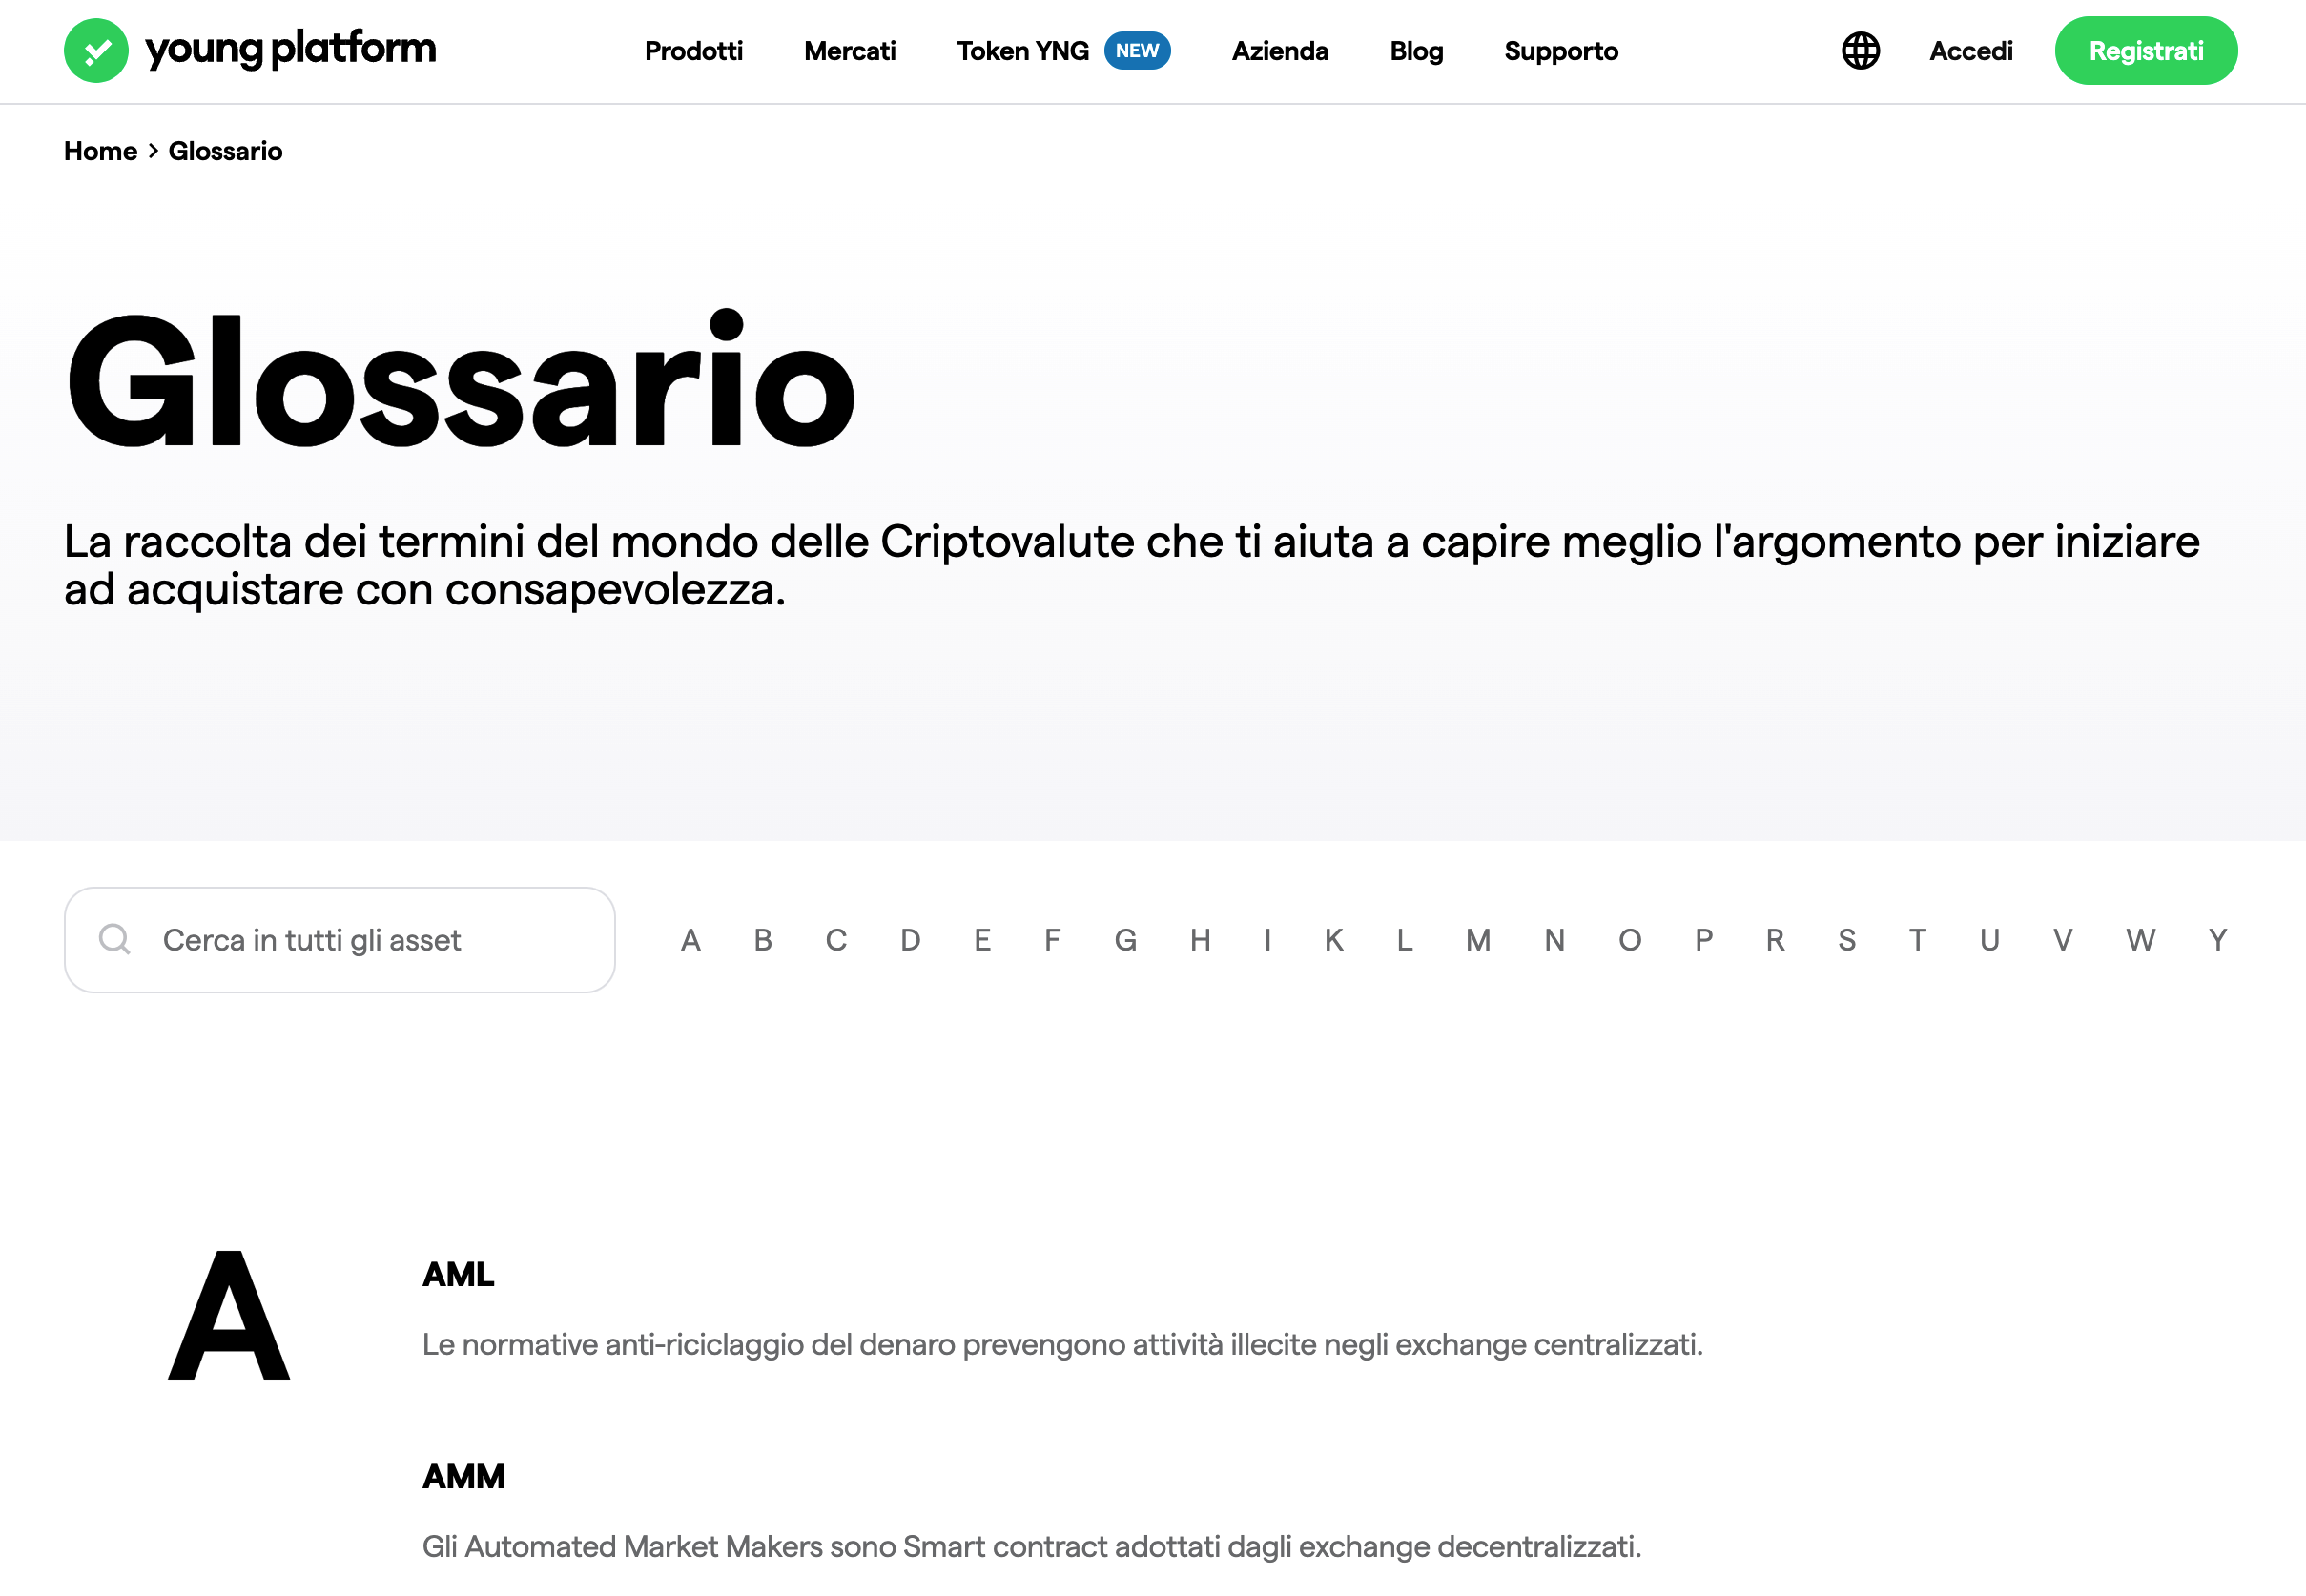
\includegraphics[width=0.80\textwidth]{res/images/internal-pages/glossary/glossary-1.png}
  \caption{Glossary page.}
  \label{fig:glossary-1}
\end{figure}

\paragraph{Who}

Il logo aziendale è sempre presente in alto a sinistra, come illustrato 
nella figura \ref{fig:glossary-1}.

\paragraph{Where}

Anche in questa pagina è presente un \textit{breadcrumb} e permette 
all'utente di non rimanere disorientato. L'utilizzo di questo elemento 
permette di comunicare in maniera efficace gran parte dell'asse where 
(in alto a sinistra, sotto al logo aziendale) (fig. \ref{fig:glossary-1}).

\paragraph{Why}

Un utente principiante ha maggiori motivi di esplorare questa pagina, in 
quanto, si suppone, che per un utente esperto questi termini siano già 
ben conosciuti.

\paragraph{When}

In questa pagina non è presente alcun riferimento temporale.

\paragraph{How}

Questa pagina è difficile da raggiungere, in quanto bisogna recarsi nel 
footer del sito (seconda voce della seconda colonna) (fig. \ref{fig:footer}). 
Questo è uno svantaggio importante sopratutto per un utente principiante: 
questa pagina, dal suo punto di vista, ha un enorme importanza, in quanto 
rappresenta un punto di riferimento per comprendere il significato di una 
miriade di termini tecnici del settore. Quindi, questa pagina dovrebbe 
affiancata a pagine molto importanti e utili (ad esempio, il blog) e 
facilmente raggiungibile. Questa pagina predispone due strumenti per la 
ricerca di specifici termini (fig. \ref{fig:glossary-2}):

\begin{figure}[H]
  \centering
  
\includegraphics[width=0.80\textwidth]{res/images/internal-pages/glossary/glossary-2.png}
  \caption{Strumenti di ricerca per i termini nel glossario.}
  \label{fig:glossary-2}
\end{figure}

\begin{itemize}
  \item A sinistra vi è una barra di ricerca in cui l'utente può digitare 
  un termine e trovare, quindi, il suo significato. Per ogni carattere che 
  viene digitato, il sito propone tutti i termini correlati ai caratteri 
  fino a quel momento inseriti, così da visualizzare anche altri termini 
  simili o correlati;
  \item A destra sono presenti le lettere dell'alfabeto, di cui ognuna 
  può essere cliccata. Se si clicca su una di queste lettere, il sito 
  proporrà tutti i termini che iniziano con tale lettera. In figura 
  \ref{fig:glossary-3} è possibile vedere un esempio. Questo strumento è 
  molto utile per gli utenti che non hanno ancora dimistichezza con i vari 
  termini di questo settore e pertanto potrebbero non ricordare il nome 
  esatto di un termine.
\end{itemize}

\begin{figure}[H]
  \centering
  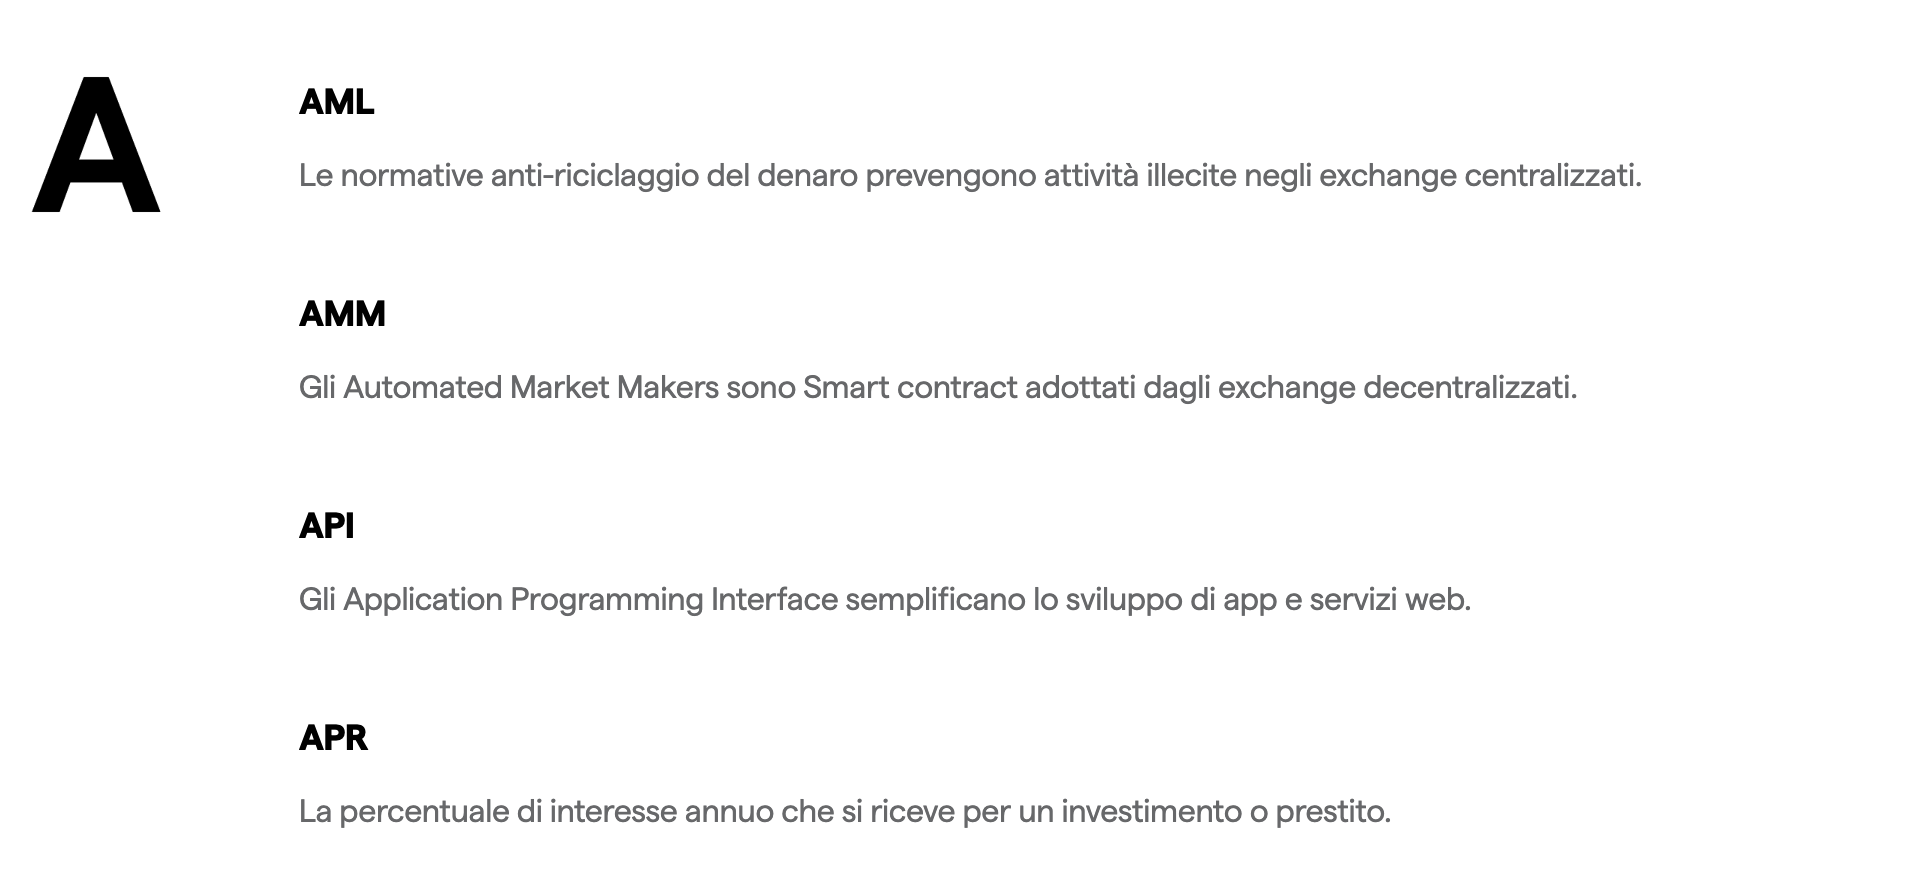
\includegraphics[width=0.80\textwidth]{res/images/internal-pages/glossary/glossary-3.png}
  \caption{Alcuni risultati per la lettera \textit{A}.}
  \label{fig:glossary-3}
\end{figure}

\subsubsection{Page of a term of the glossary}

La pagina a cui si fa riferimento è raggiungibile al seguente indirizzo \\
\href{https://youngplatform.com/glossary/api/}{https://youngplatform.com/glossary/api/}.

\paragraph{What}

Il contenuto di questa pagina esplicita chiaramente il suo obiettivo, ovvero, 
quello di fornire il significato di un termine scelto precedentemente 
dall'utente.

\begin{figure}[H]
  \centering
  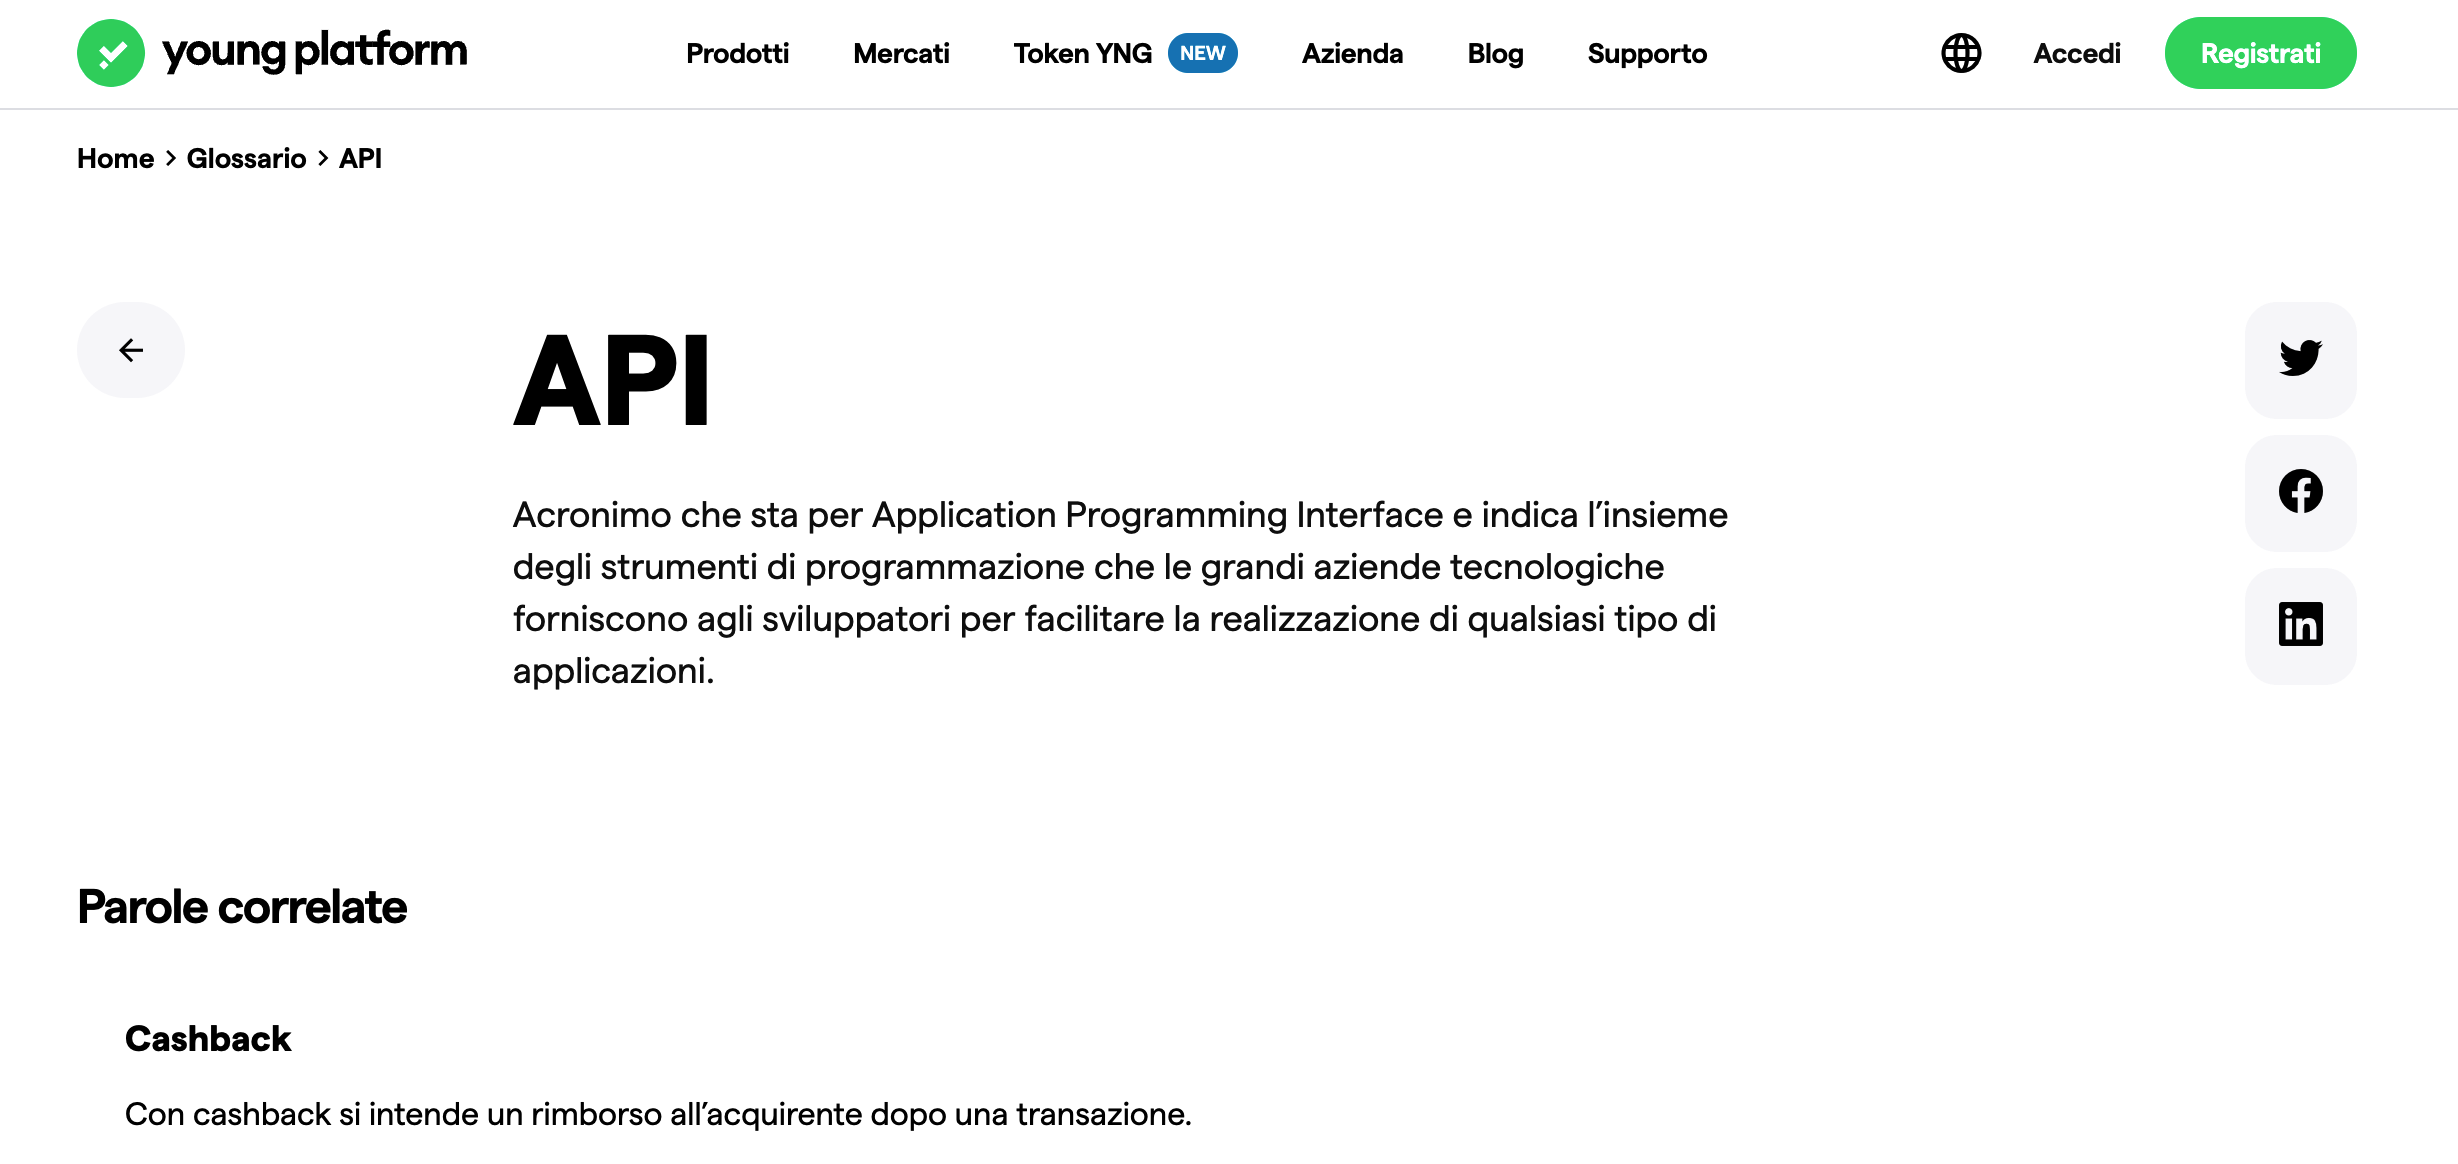
\includegraphics[width=0.80\textwidth]{res/images/internal-pages/glossary/glossary-4.png}
  \caption{Pagina che descrive il significato del termine \textit{API}.}
  \label{fig:glossary-4}
\end{figure}

\paragraph{Who}

Il logo aziendale è sempre presente in alto a sinistra, come illustrato 
nella figura \ref{fig:glossary-4}.

\paragraph{Where}

Anche in questa pagina è presente un \textit{breadcrumb} e permette 
all'utente di non rimanere disorientato. L'utilizzo di questo elemento 
permette di comunicare in maniera efficace gran parte dell'asse where 
(in alto a sinistra, sotto al logo aziendale) (fig. \ref{fig:glossary-4}). 
C'è un altro elemento nella pagina che aumenta l'usabilità del sito: 
in figura \ref{fig:academy-4} a sinistra c'è una freccia che permette di 
tornare indietro, ovvero, al \textit{Glossario}. 

\paragraph{Why}

Un utente neofita ha più motivi di un utente esperto di rimanere in questa 
pagina, in quanto un principiante ha raggiunto questa pagina per informarsi 
su un contenuto molto specifico. Inoltre, dopo la definizione del termine 
cercato, è presente una sezione in cui vi è una lista di termini 
strettamente correlati al termine cercato (fig. \ref{fig:glossary-5}). 
Questa sezione è molto importante perchè l'utente può cercare diversi 
termini e che seguono tutti un filo conduttore a partire dal termine 
cercato inizialmente. 

\begin{figure}[H]
  \centering
  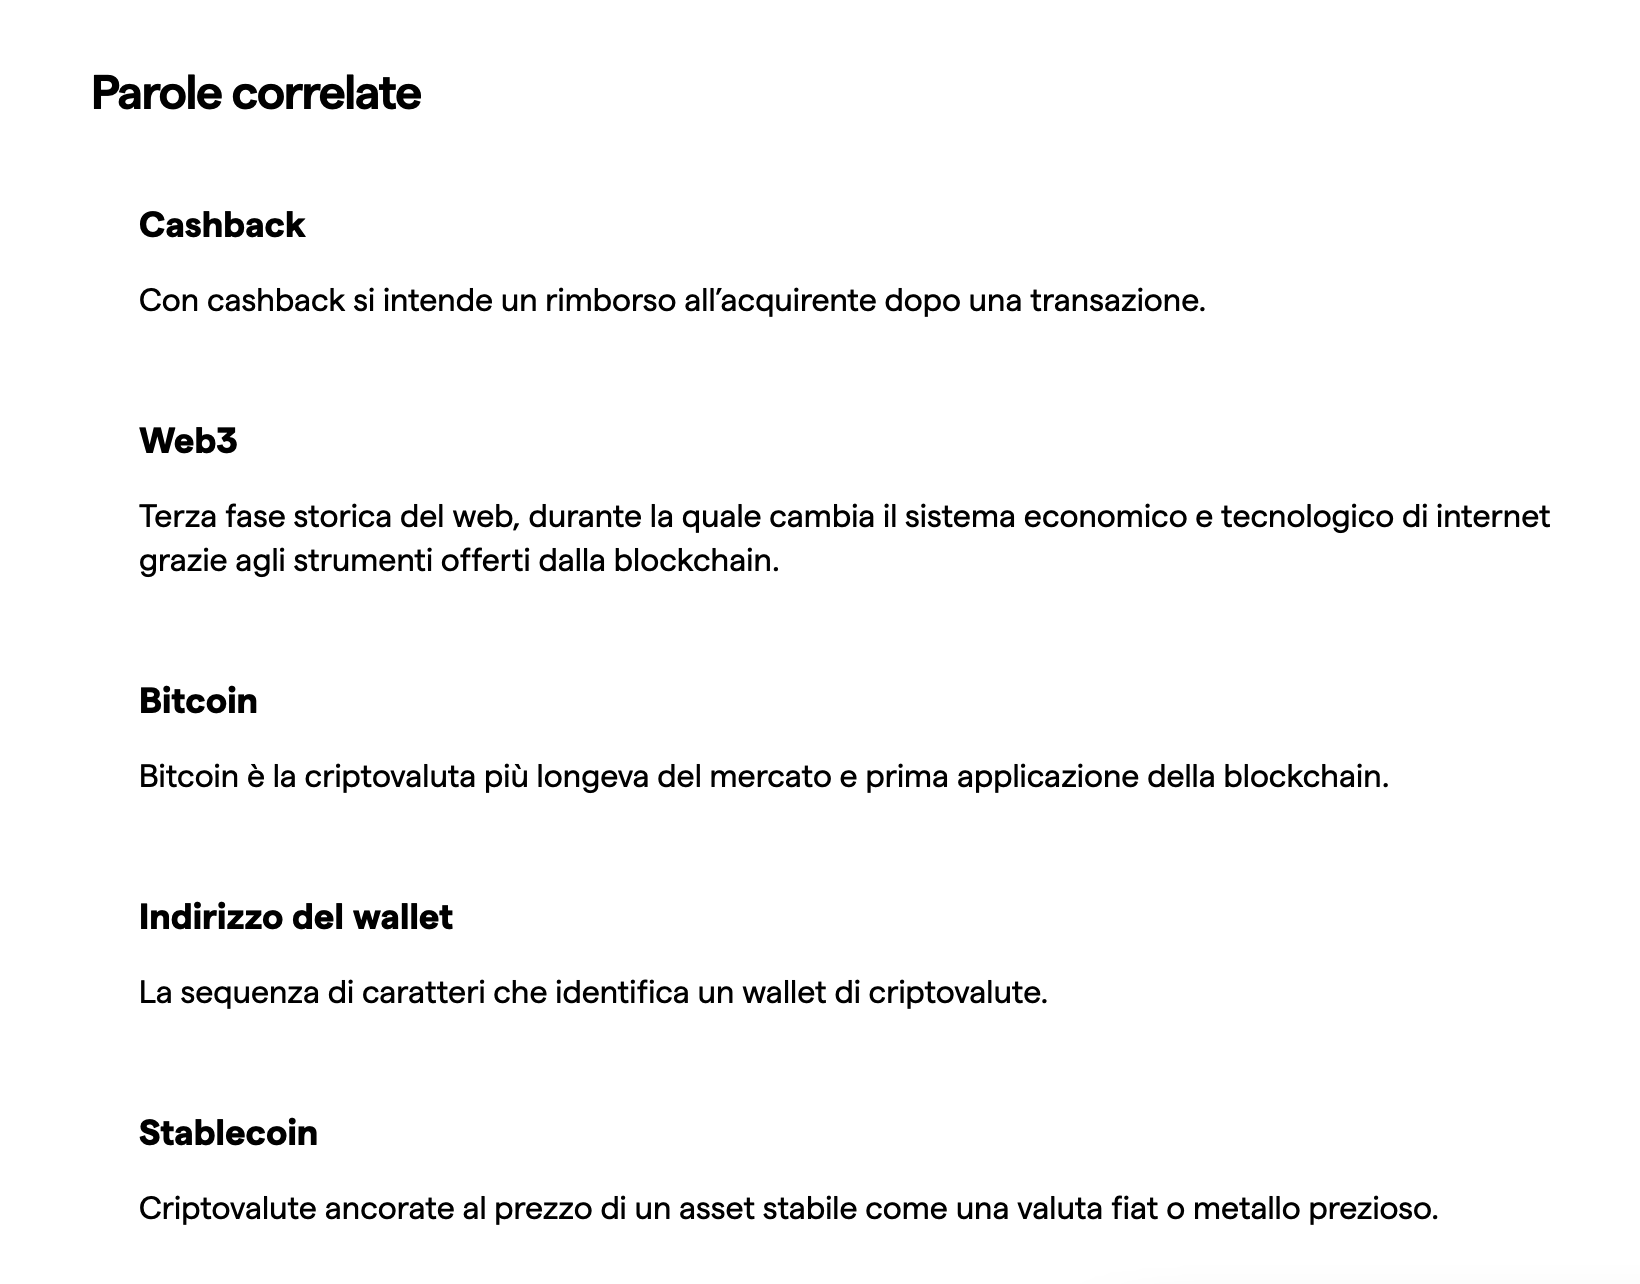
\includegraphics[width=0.80\textwidth]{res/images/internal-pages/glossary/glossary-5.png}
  \caption{Termini correlati a partire dal termine \textit{API}.}
  \label{fig:glossary-5}
\end{figure}

\paragraph{When}

In questa pagina non è presente alcun riferimento temporale.

\paragraph{How}

Questa pagina specifica è difficile da raggiungere. Tuttavia, l'accesso 
a tale pagina è facilitata se si accede al \textit{Glossario}, in quanto 
sono presenti degli strumenti che facilitano il raggiungimento di questa 
pagina.

\subsubsection{Blog page}

La pagina a cui si fa riferimento è raggiungibile al seguente indirizzo 
\href{https://youngplatform.com/blog/}{https://youngplatform.com/blog/}.

\paragraph{What}

Gli intenti di questa pagina sono esplicitati, ovvero, quello di fornire 
una serie di contenuti, in modo che gli utenti possano rimanere aggiornati 
su tutte le ultime novità di questo settore. Inoltre, i vari articoli 
vengono anche catalogati, in modo da capire anche il contesto di cui 
trattano.

\begin{figure}[H]
  \centering
  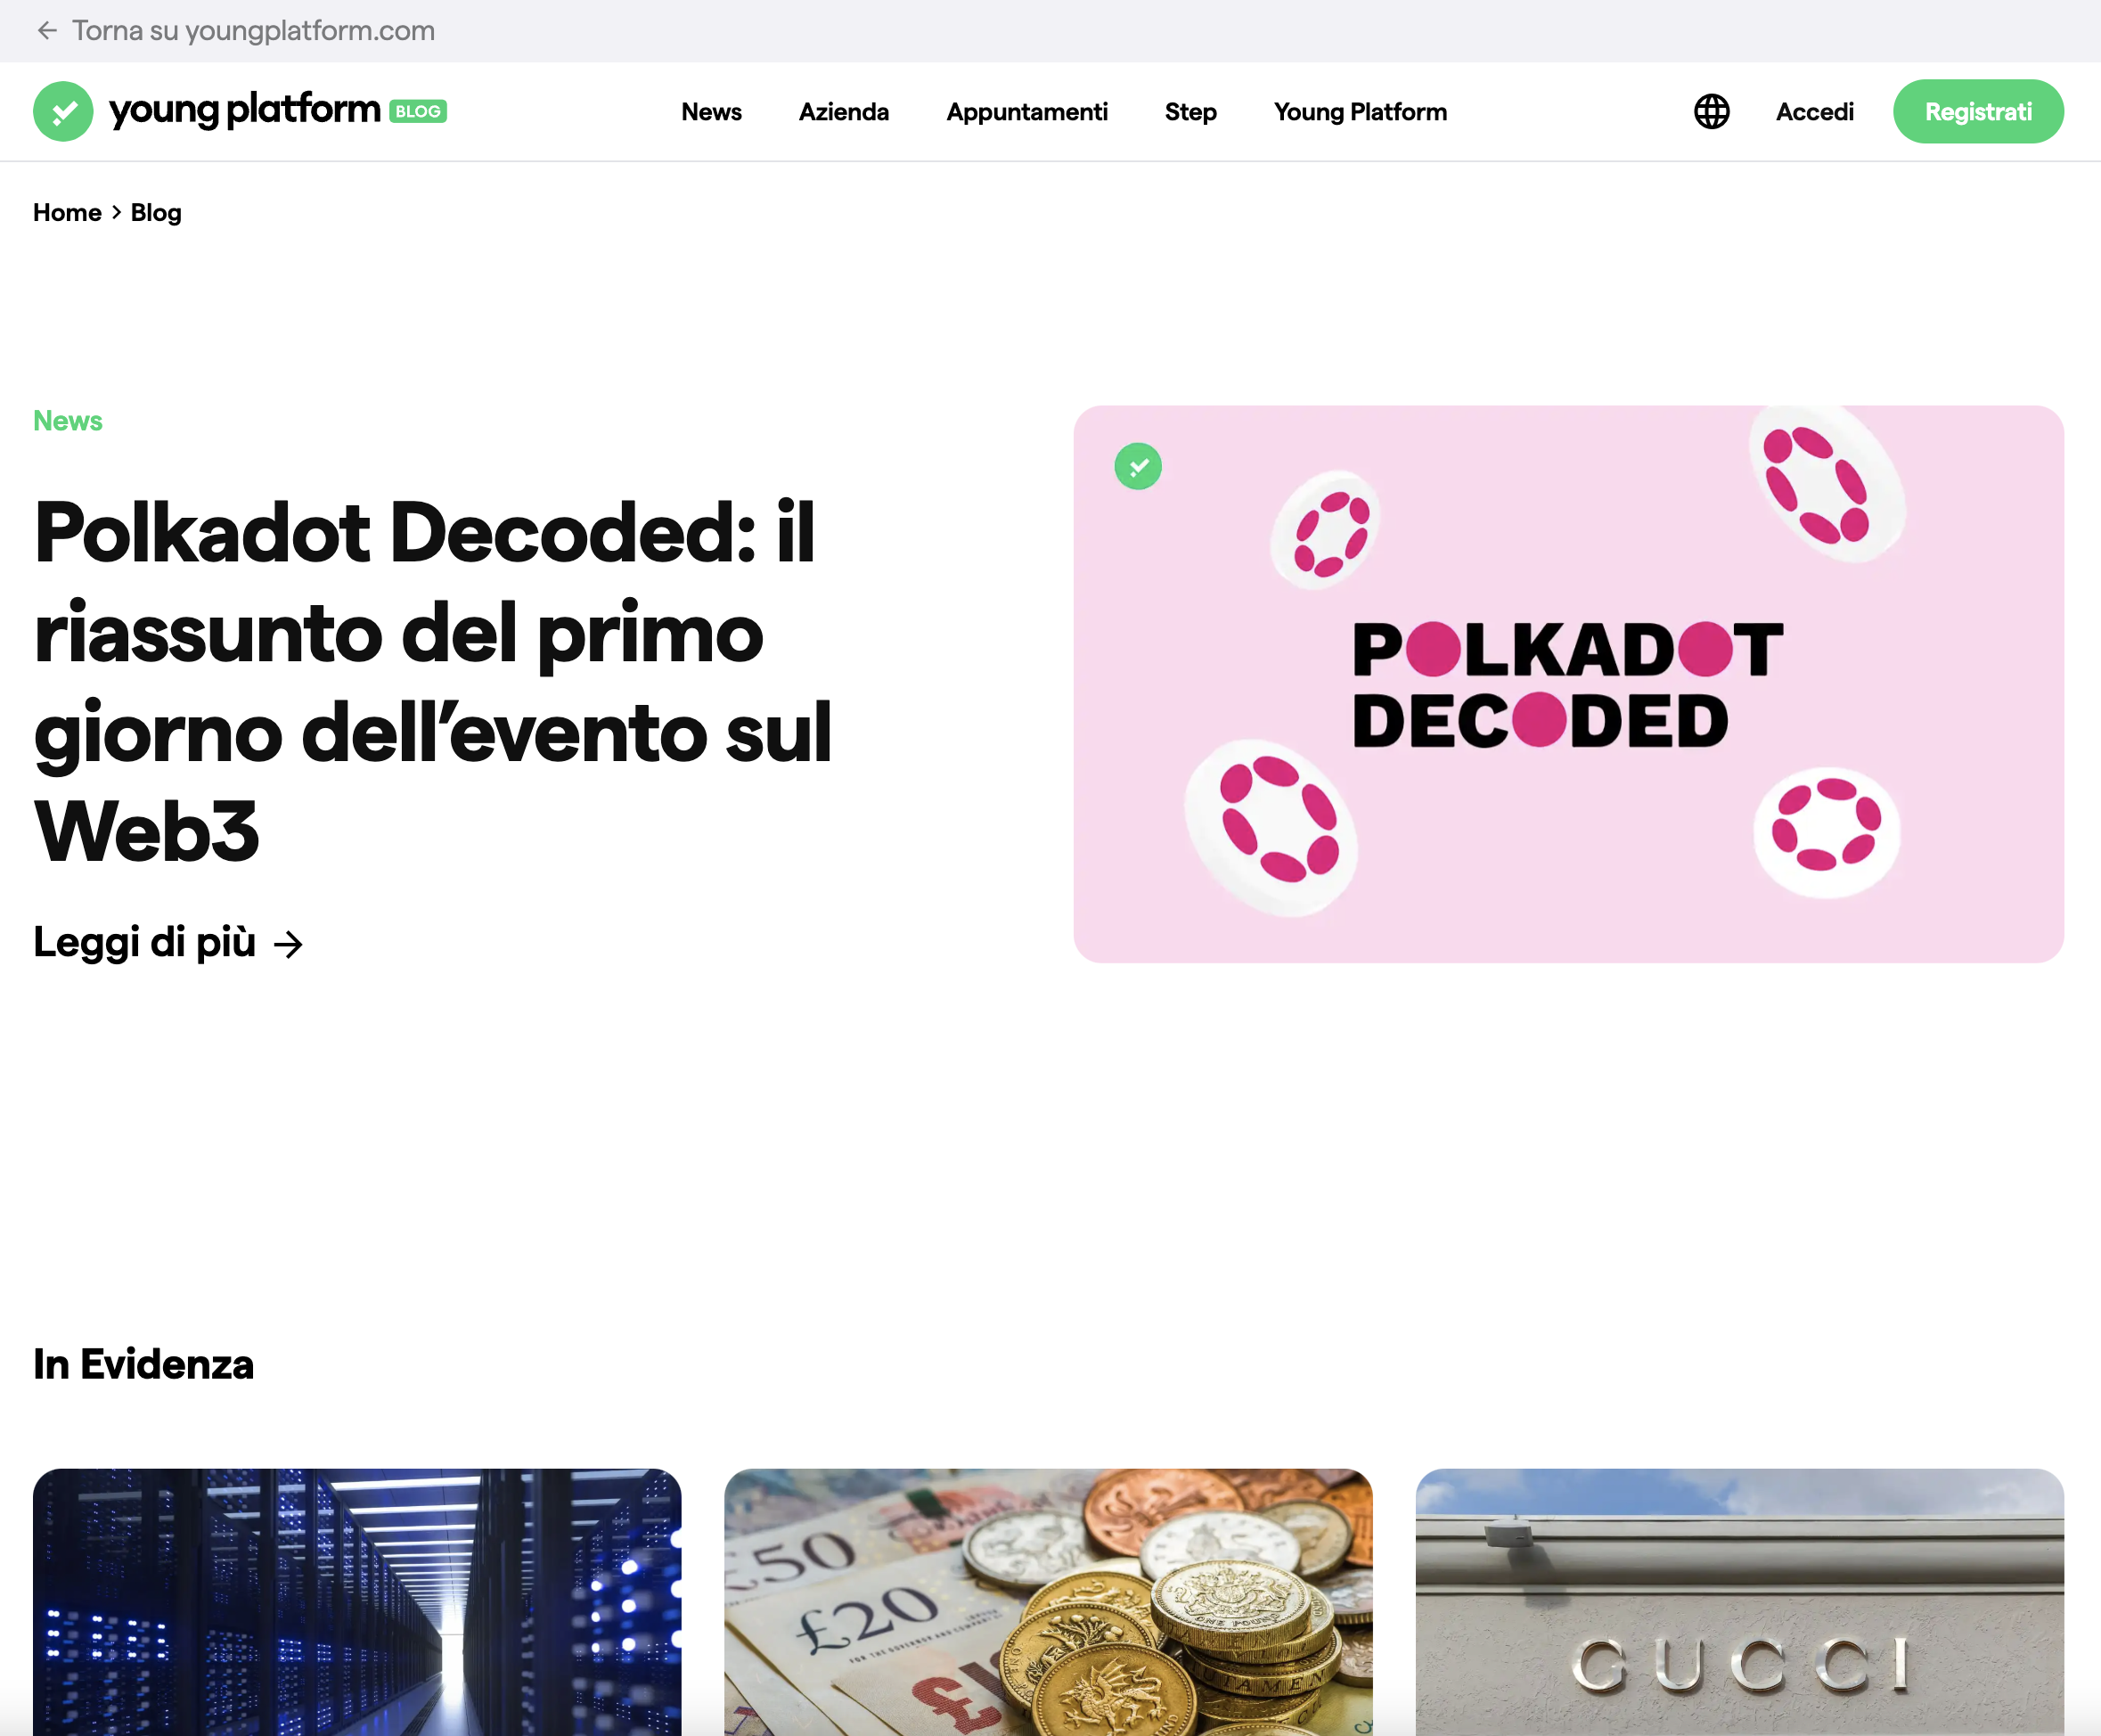
\includegraphics[width=0.80\textwidth]{res/images/internal-pages/blog/blog-1.png}
  \caption{Blog page.}
  \label{fig:blog-1}
\end{figure}

\paragraph{Who}

Il logo aziendale è sempre presente in alto a sinistra, come illustrato 
nella figura \ref{fig:blog-1}.

\paragraph{Where}

Anche in questa pagina è presente un \textit{breadcrumb} e permette 
all'utente di non rimanere disorientato. L'utilizzo di questo elemento 
permette di comunicare in maniera efficace gran parte dell'asse where 
(in alto a sinistra, sotto al logo aziendale) (fig. \ref{fig:blog-1}). 
C'è un altro elemento nella pagina che aumenta l'usabilità del sito: 
in figura \ref{fig:blog-1}, sopra il logo aziendare, c'è una freccia e 
un testo \textit{Torna su youngplatform.com}. Questo rappresenta un 
punto di riferimento per tornare direttamente alla homepage.

\paragraph{Why}

Indipendentemente dall'esperienza dell'utente, i motivi per cui continuare 
ad esplorare questa sono:
\begin{itemize}
  \item Per rimanere aggiornati sulle ultime novità tecnologiche;
  \item Per rimanere aggiornati sulle ultime novità del mercato;
  \item Per confrontare diversi approcci tecnologici;
  \item Per imparare differenti concetti, in particolare per i neofiti.
\end{itemize}

\paragraph{When}

In questa pagina ci sono dei chiari riferimenti temporali: è possibile 
notare che gli articoli nella pagina sono presenti le date di pubblicazione 
(fig. \ref{fig:blog-2}). Inoltre, come illustrato nella figura 
\ref{fig:blog-1}, nella sezione iniziale di questa pagina viene posto 
l'ultimo articolo pubblicato, mettendolo in evidenza. 

\paragraph{How}

Questa pagina può facilmente essere raggiunta tramite il menù principale 
della homepage (quinta voce) (fig. \ref{fig:homepage-1}). Tuttavia, se un 
utente volesse cercare un articolo particolare, questo non è possibile 
in quanto manca uno strumento di ricerca. Questo rappresenta un grave 
svantaggio. Per poter trovare un particolare articolo, l'utente dovrebbe 
cercarlo tramite un motore di ricerca, specificando il sito. Scorrendo la 
pagina, è possibile vedere che gli articoli sono catalogati e ogni categoria 
ha una voce \textit{Vedi tutti} (in alto a destra, fig. \ref{fig:blog-2}), 
in cui si viene reindirizzati in una pagina che contiente tutti gli articoli 
di tale categoria. Tali categorie sono riporate anche ad inizio pagina, 
a fianco del logo aziendale. Questo permette ad un utente di avere già 
una panoramica delle varie categorie e se un utente ha già in mente che 
tipologia di articolo cerca, questo facilita il raggiungimento 
dell'articolo. Tuttavia, la scelta di cambiare le voci del menù principale 
rispetto a quelle della homepage, potrebbe causare un senso di 
disorientamento nell'utente.

\begin{figure}[H]
  \centering
  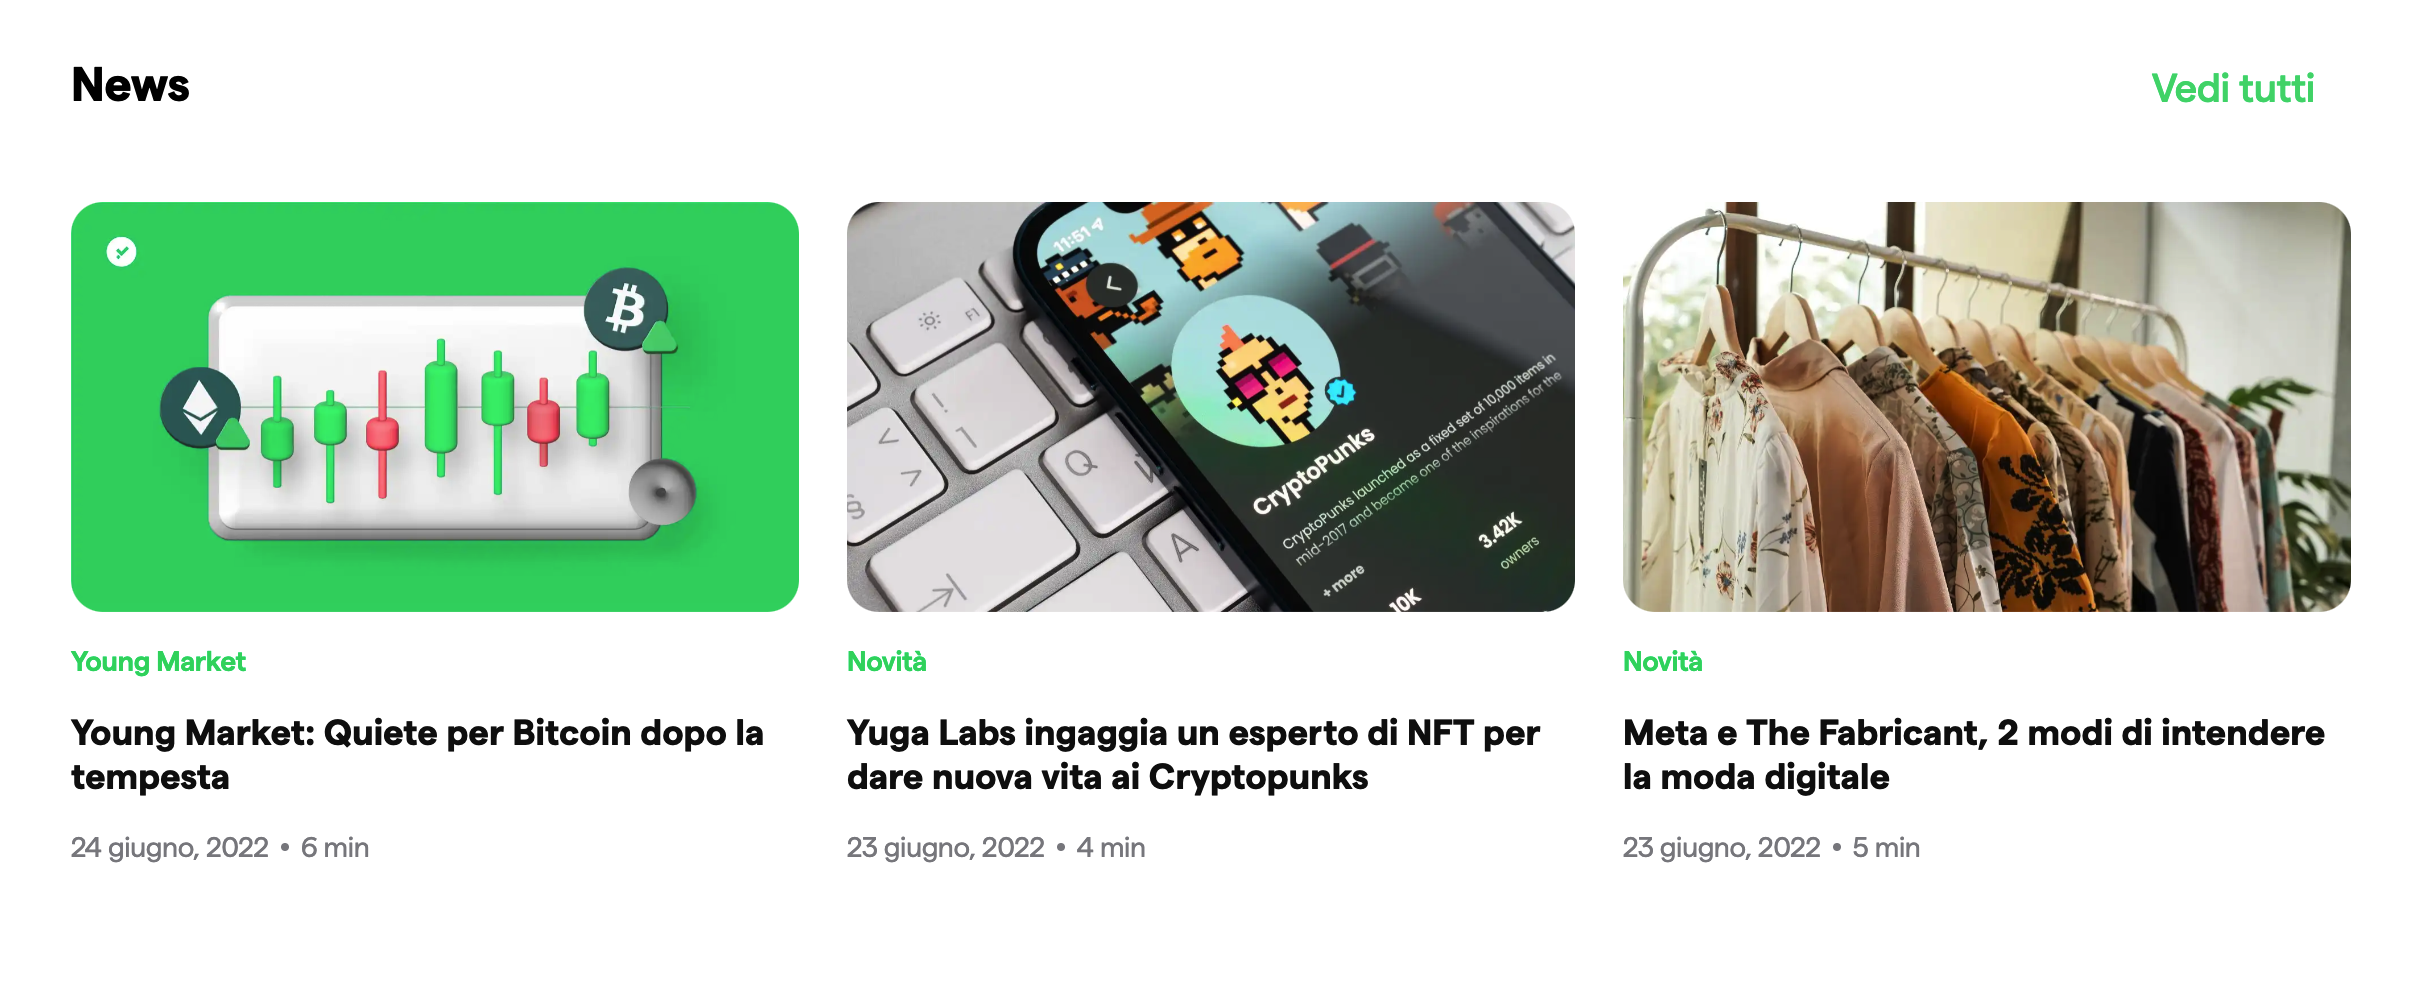
\includegraphics[width=0.80\textwidth]{res/images/internal-pages/blog/blog-2.png}
  \caption{Una delle categorie presente nella pagina Blog.}
  \label{fig:blog-2}
\end{figure}

\subsubsection{A blog article}

La pagina a cui si fa riferimento è raggiungibile al seguente indirizzo \\
\href{https://youngplatform.com/blog/news/mercato-crypto-quiete-bitcoin-dopo-tempesta/}{https://youngplatform.com/blog/news/mercato-crypto-quiete-bitcoin-dopo-tempesta/}.

\paragraph{What}

L'obiettivo di questa pagina specifica è esplicitato chiaramente dal 
titolo. Infatti, il titolo introduce quello che sarà il contenuto 
dell'articolo.

\begin{figure}[H]
  \centering
  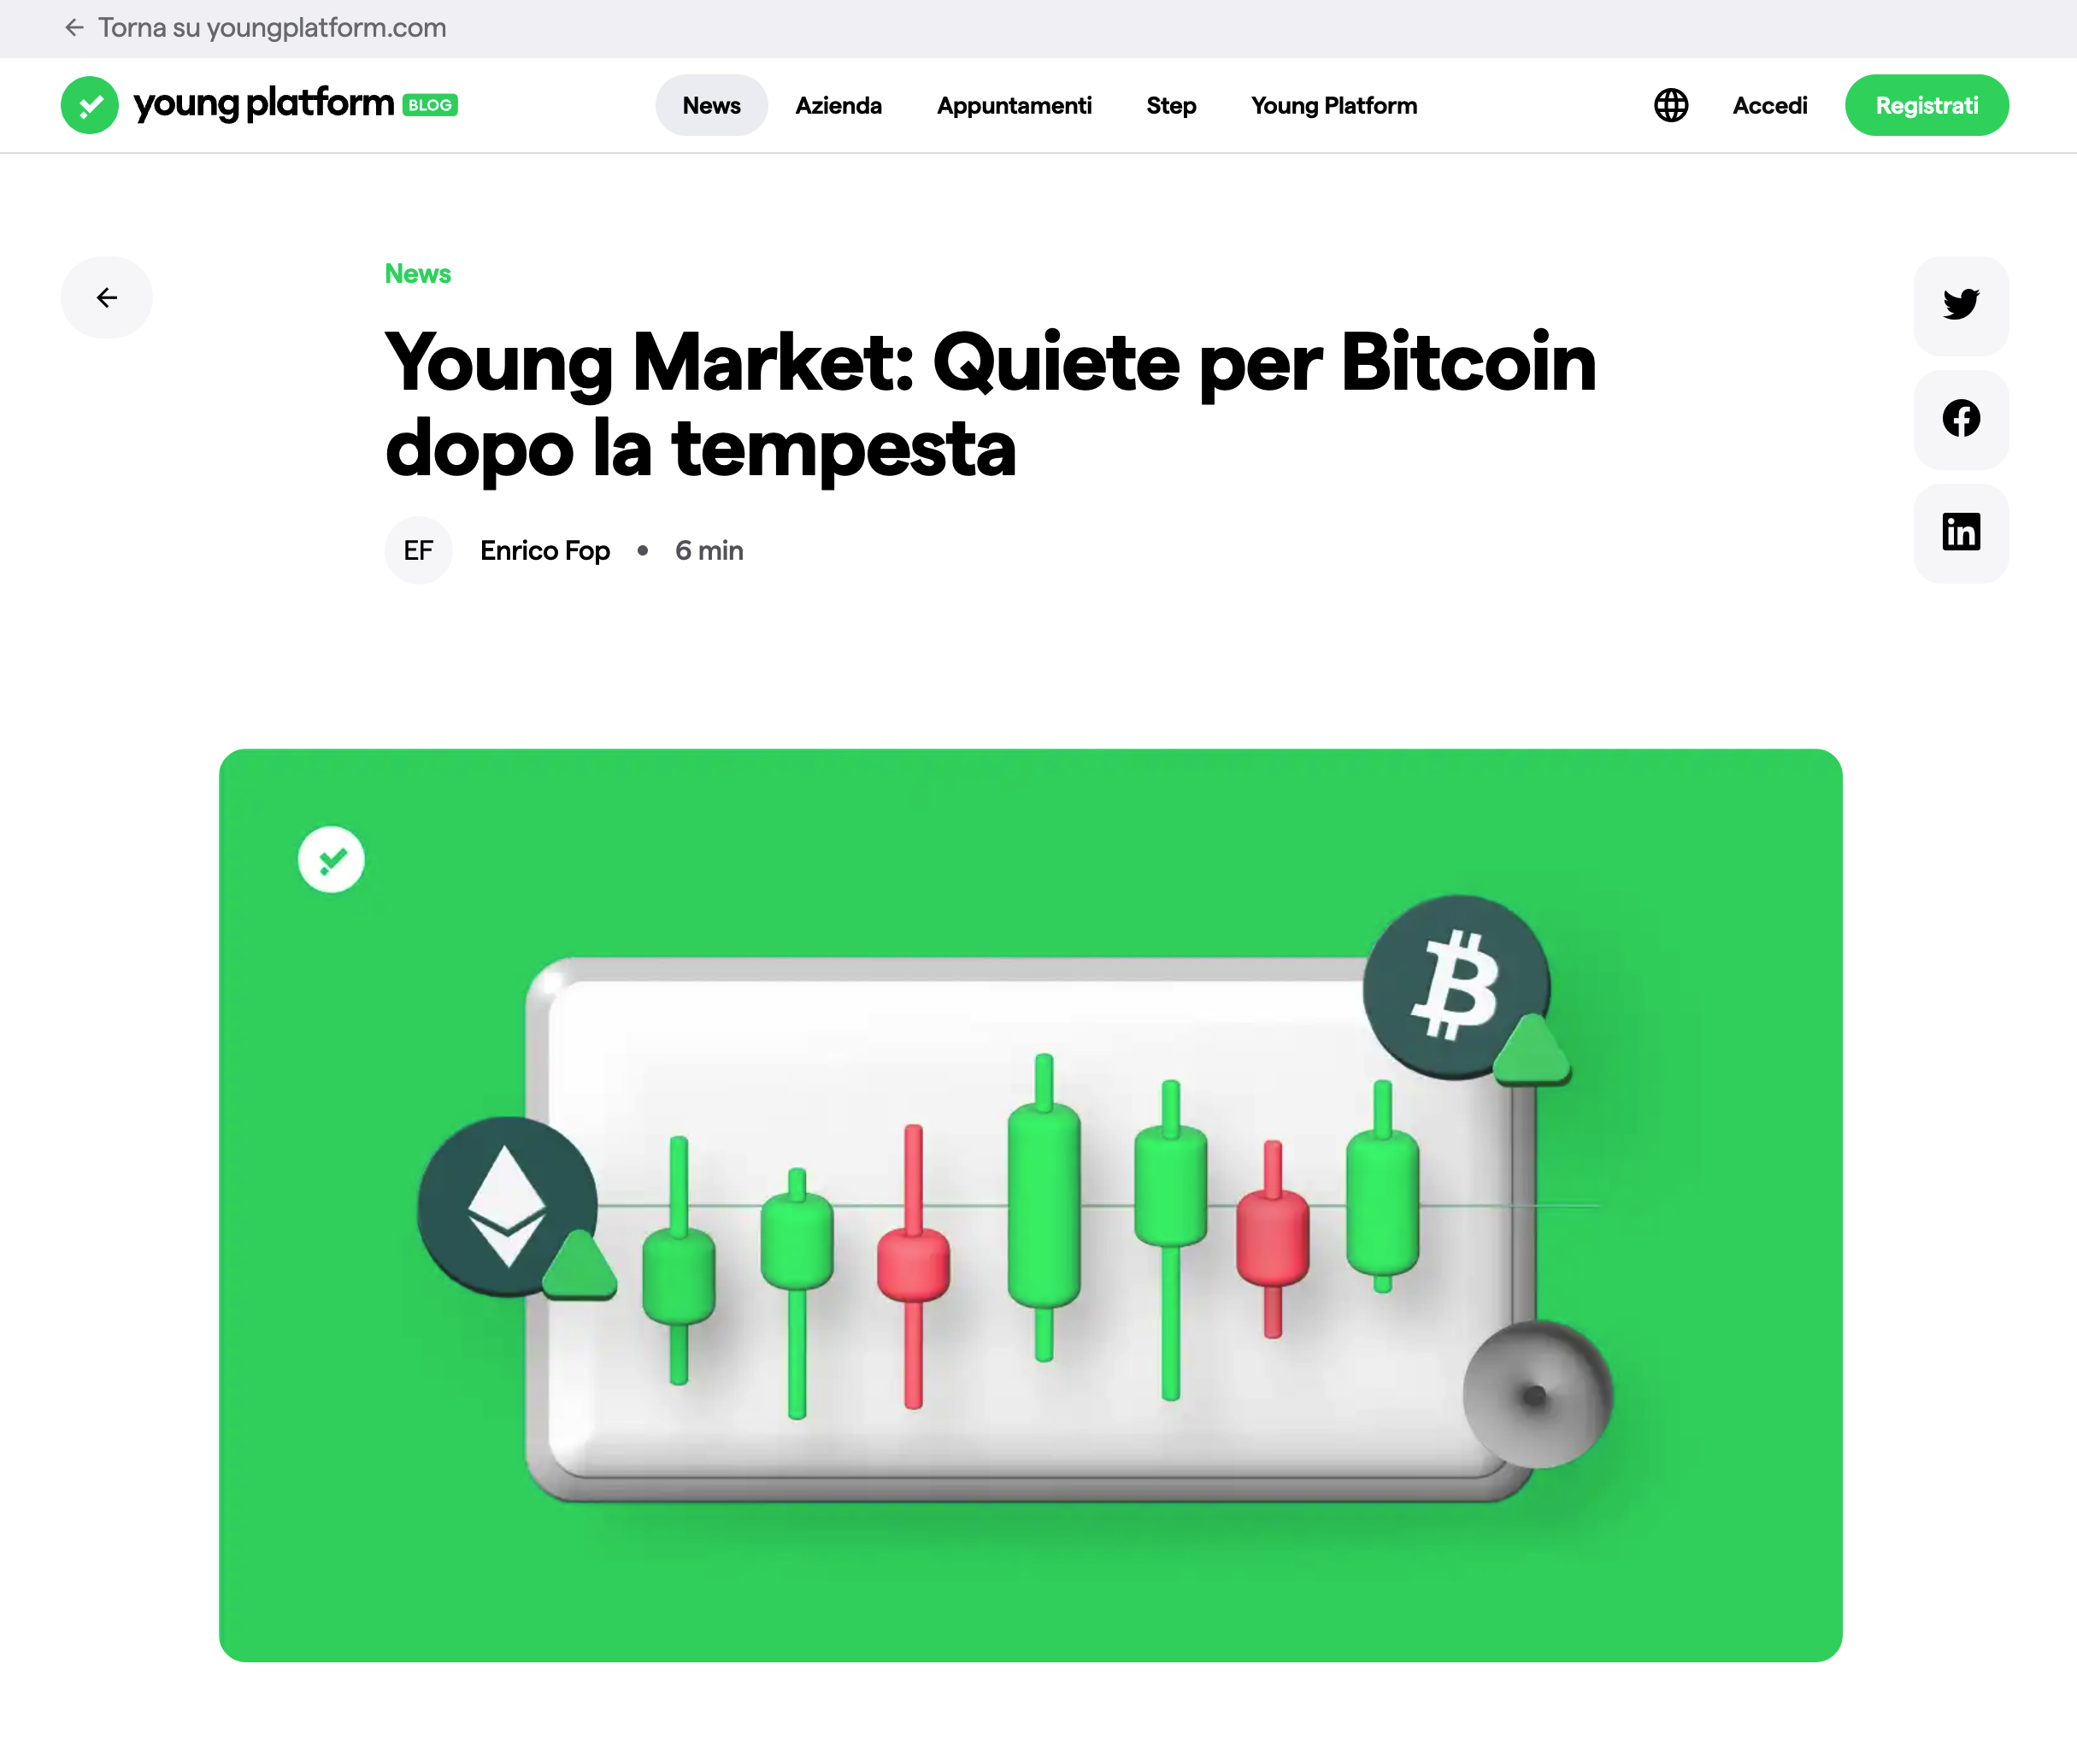
\includegraphics[width=0.80\textwidth]{res/images/internal-pages/blog/blog-3.png}
  \caption{Un articolo del blog.}
  \label{fig:blog-3}
\end{figure}

\paragraph{Who}

Il logo aziendale è sempre presente in alto a sinistra, come illustrato 
nella figura \ref{fig:blog-3}.

\paragraph{Where}

Anche in questa pagina è presente un \textit{breadcrumb} e permette 
all'utente di non rimanere disorientato. L'utilizzo di questo elemento 
permette di comunicare in maniera efficace gran parte dell'asse where 
(in alto a sinistra, sotto al logo aziendale) (fig. \ref{fig:blog-3}). 
C'è un altro elemento nella pagina che aumenta l'usabilità del sito: 
in figura \ref{fig:blog-3} a sinistra c'è una freccia che permette di 
tornare indietro, nella pagine del blog. Tale elemento rimane sempre nella 
stessa posizione anche se l'utente scorre la pagina. Questo è un aspetto 
postivo perchè se l'utente vuole tornare alla pagina precedente, non è 
necessario che l'utente ritorni ad inizio pagina. Inoltre, in figura 
\ref{fig:blog-3}, sopra il logo aziendare, c'è una freccia e un testo 
\textit{Torna su youngplatform.com}. Questo rappresenta un punto di 
riferimento per tornare direttamente alla homepage. Rispetto agli articoli 
della \textit{Academy}, non c'è la barra che evidenzia a che punto è 
arrivato l'utente a leggere l'articolo.

\paragraph{Why}

Il motivo principale per continuare ad esplorare la pagina è perchè 
l'utente (che sia principiante o esperto) è interessato alla lettura di 
questo specifico articolo. Inoltre, a fine pagina vi è una sezione che 
invita alla lettura di altri articoli correlati a quello appena letto.

\paragraph{When}

Nonostante nella pagina \textit{Blog} ci siano dei chiari riferimenti 
temporali, nella pagina specifica dell'articolo non c'è la data di 
pubblicazione dell'articolo.

\paragraph{How}

Il raggiungimento di questa specifica pagina è difficile. Può essere 
raggiunta tramite l'esplorazione della pagina \textit{Blog} oppure tramite 
un motore di ricerca. Questo rappresenta un grande svantaggio per l'utente, 
in quanto l'utente dovrebbe spendere molto tempo per esplorare il blog 
prima di trovare l'articolo, o dovrebbe uscire dal sito per accedere ad 
un motore di ricerca.

\subsubsection{Support page}

La pagina a cui si fa riferimento è raggiungibile al seguente indirizzo \\
\href{https://support.youngplatform.com/hc/it}{https://support.youngplatform.com/hc/it}.

\begin{figure}[H]
  \centering
  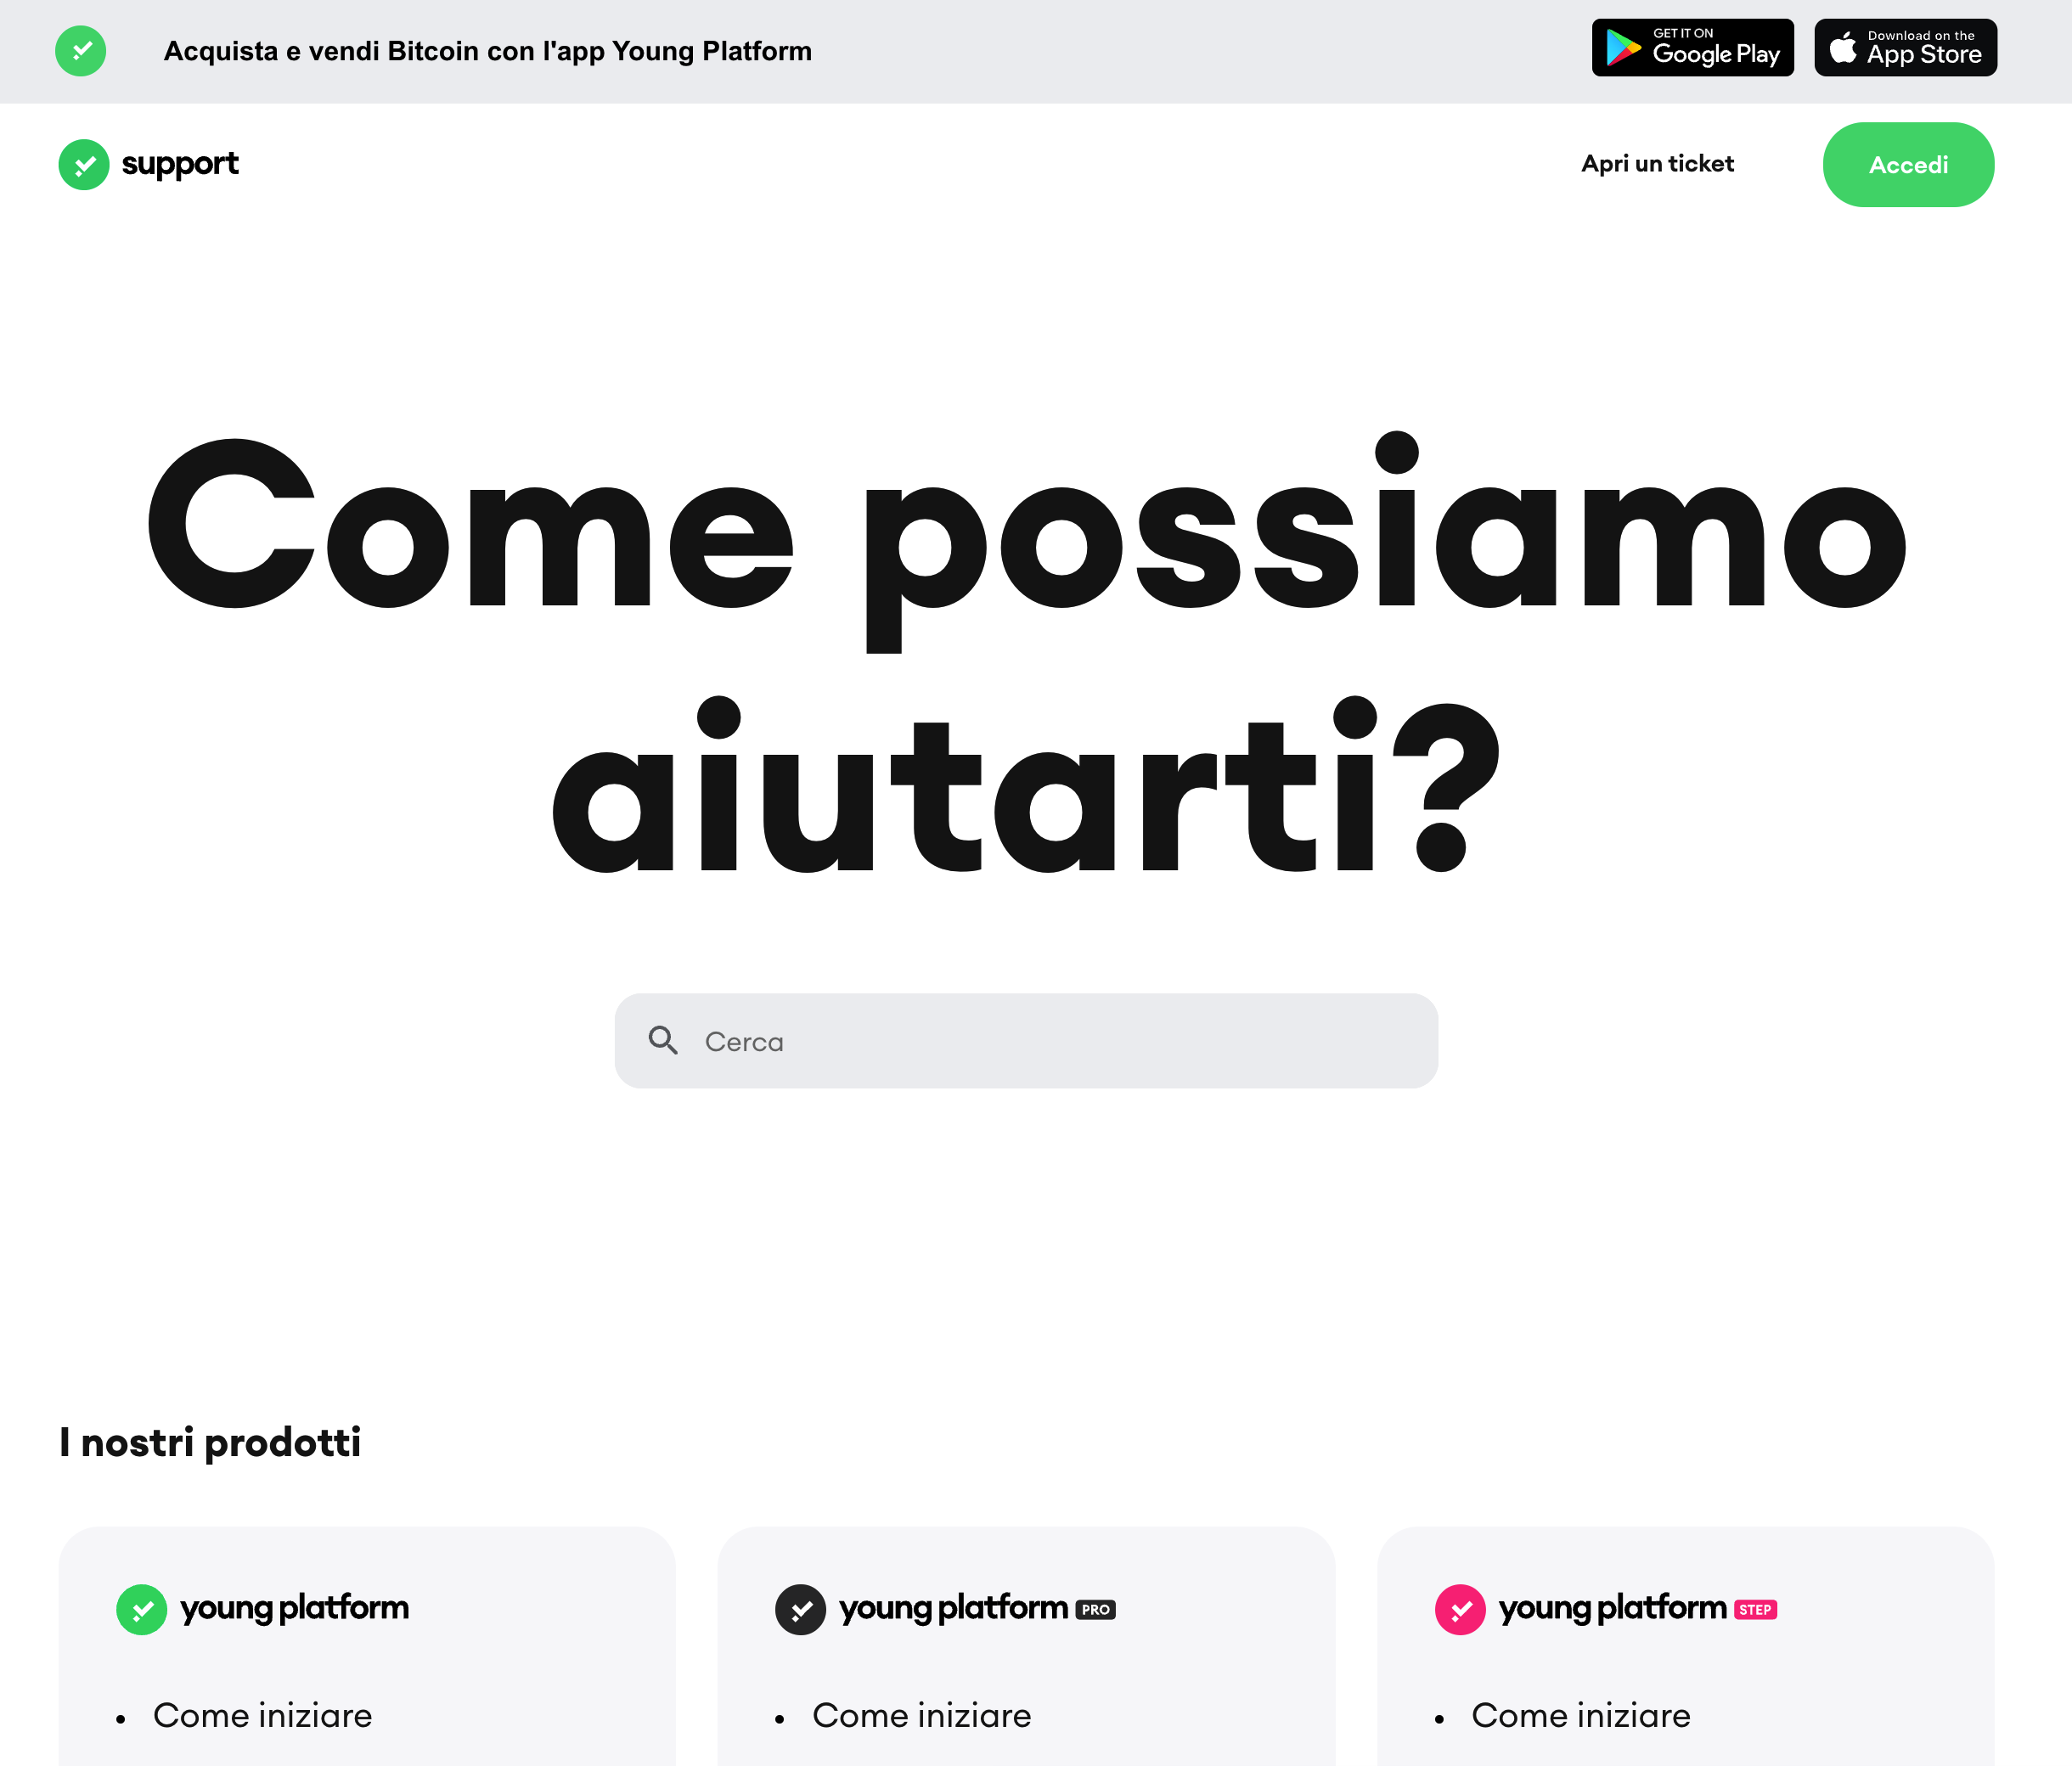
\includegraphics[width=0.70\textwidth]{res/images/internal-pages/support/support-1.png}
  \caption{First section of the \textit{Support} page.}
  \label{fig:support-1}
\end{figure}

\paragraph{What}

L'obiettivo di questa pagina è immediatamente chiaro. Lo scopo di questa 
pagina è quello di fornire supporto e aiuto all'utente. La pagina permette 
di offrire diverse "tipologie" di supporto:
\begin{itemize}
  \item \textit{Barra di ricerca}: l'utente può inserire dei termini 
  inerenti al suo problema ed ottenere dei risultati correlati 
  (fig. \ref{fig:support-2});

  \begin{figure}[H]
    \centering
    
\includegraphics[width=0.60\textwidth]{res/images/internal-pages/support/support-2.png}
    \caption{Strumento di ricerca.}
    \label{fig:support-2}
  \end{figure}
  
  \item \textit{FAQ suddivise per prodotto} (fig. \ref{fig:support-3});
  
  \begin{figure}[H]
    \centering
    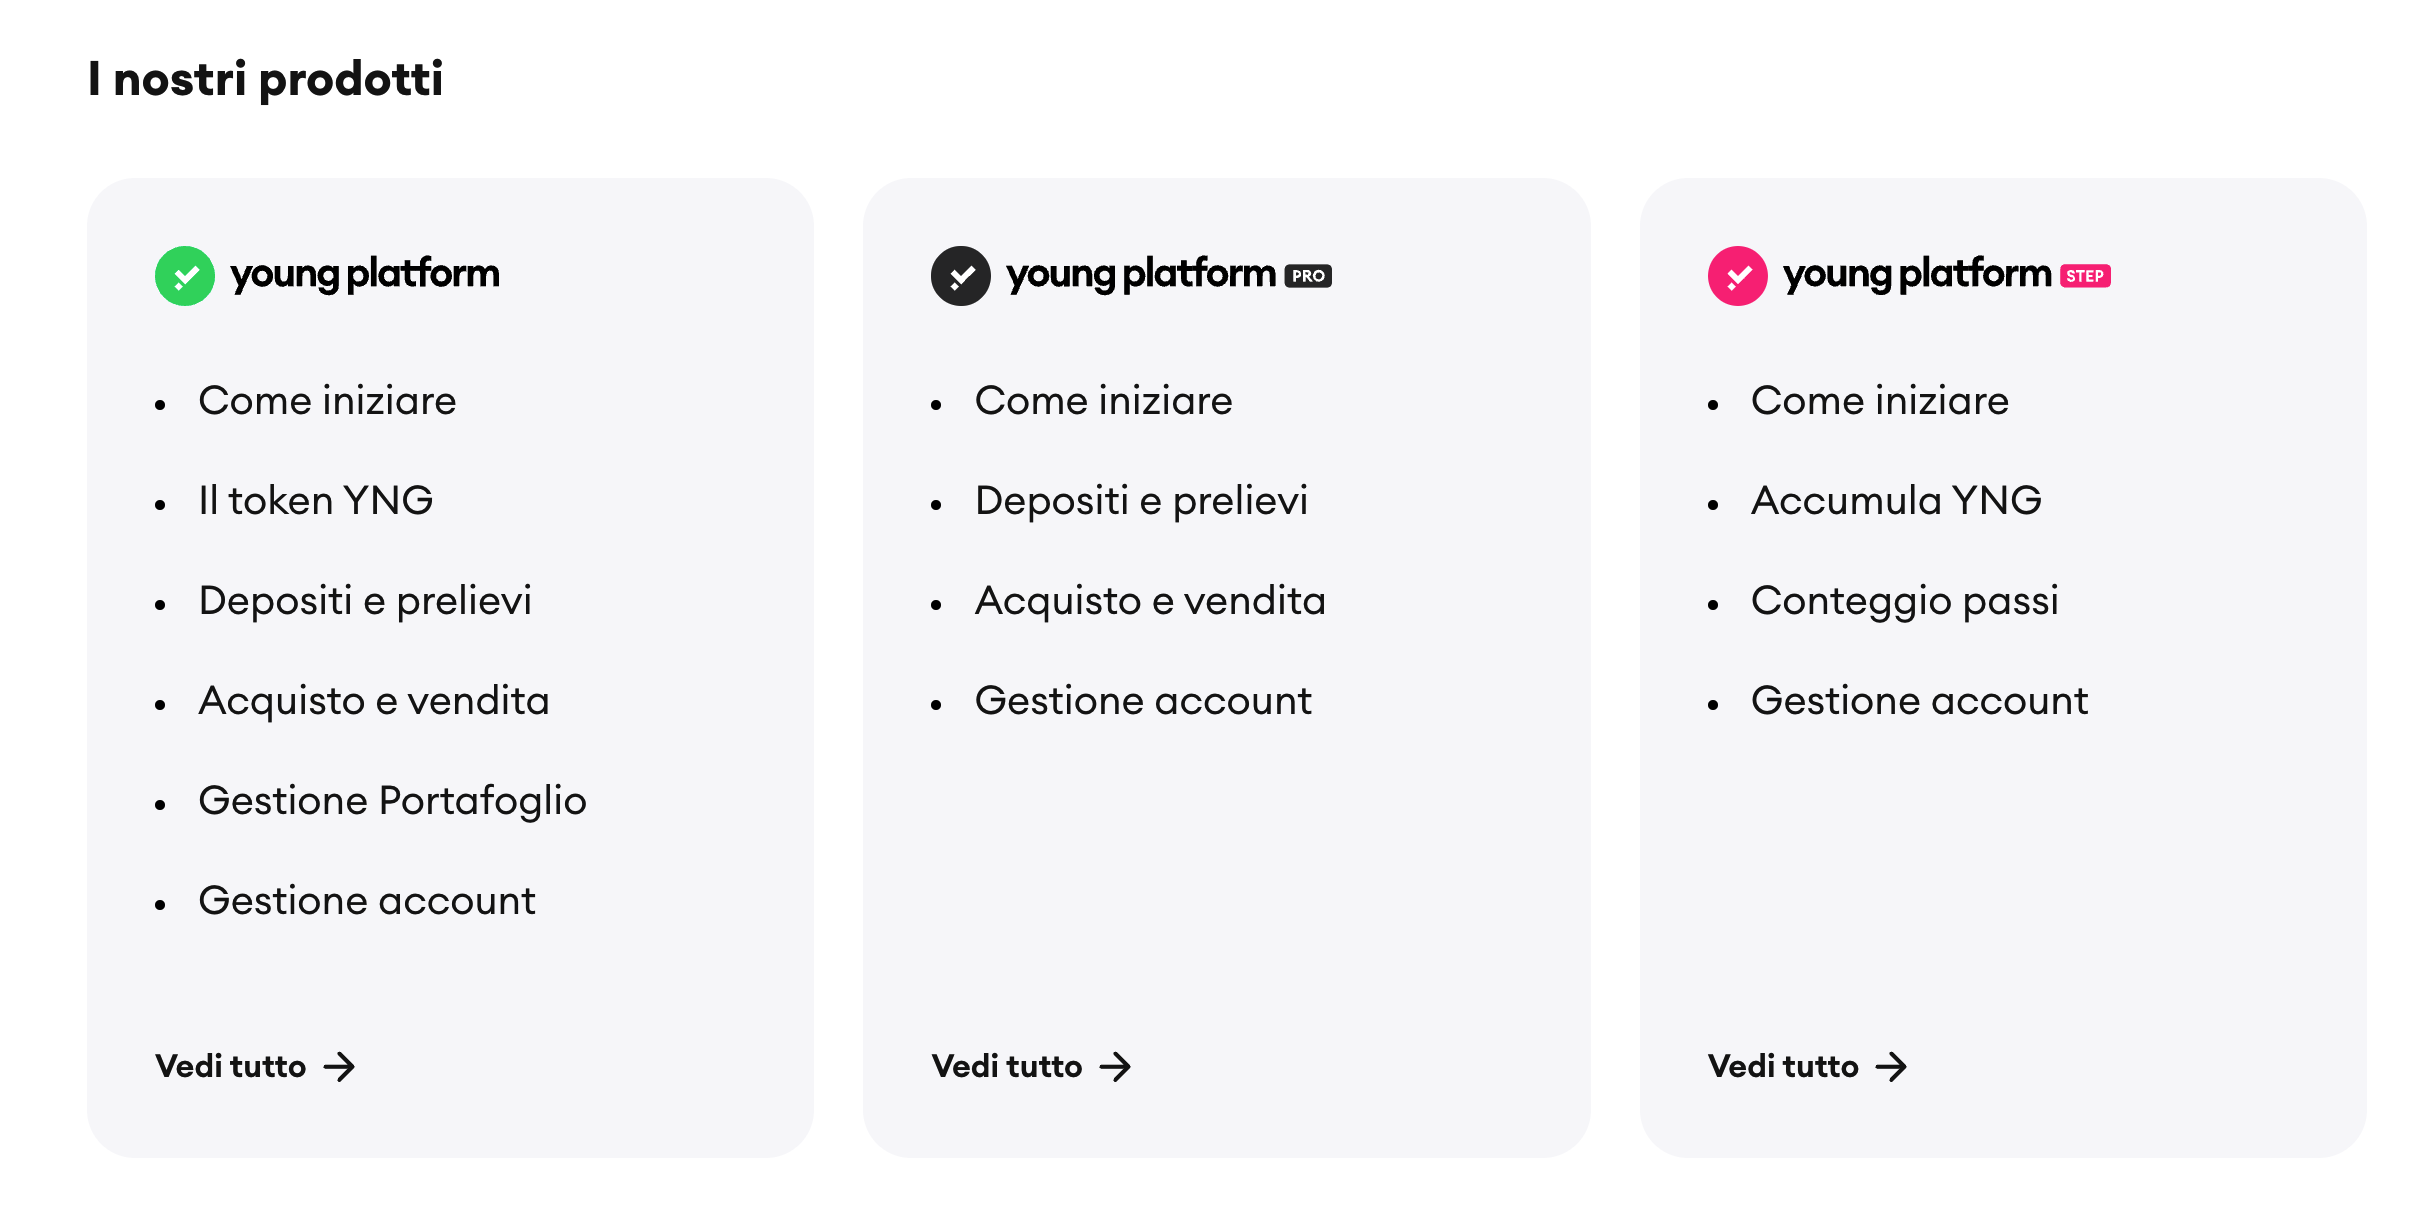
\includegraphics[width=0.80\textwidth]{res/images/internal-pages/support/support-3.png}
    \caption{Alcune FAQ suddivise per prodotto.}
    \label{fig:support-3}
  \end{figure}
  
  \item \textit{Articoli del blog} (fig. \ref{fig:support-4});
  
  \item \textit{Articoli della Academy} (fig. \ref{fig:support-5});
  
  \item \textit{Link ai social network e alla newsletter} 
  (fig. \ref{fig:support-6}).
\end{itemize}

\begin{figure}[H]
  \centering
  
\includegraphics[width=0.60\textwidth]{res/images/internal-pages/support/support-4.png}
  \caption{Sezione che reindirizza al \textit{Blog}.}
  \label{fig:support-4}
\end{figure}

\begin{figure}[H]
  \centering
  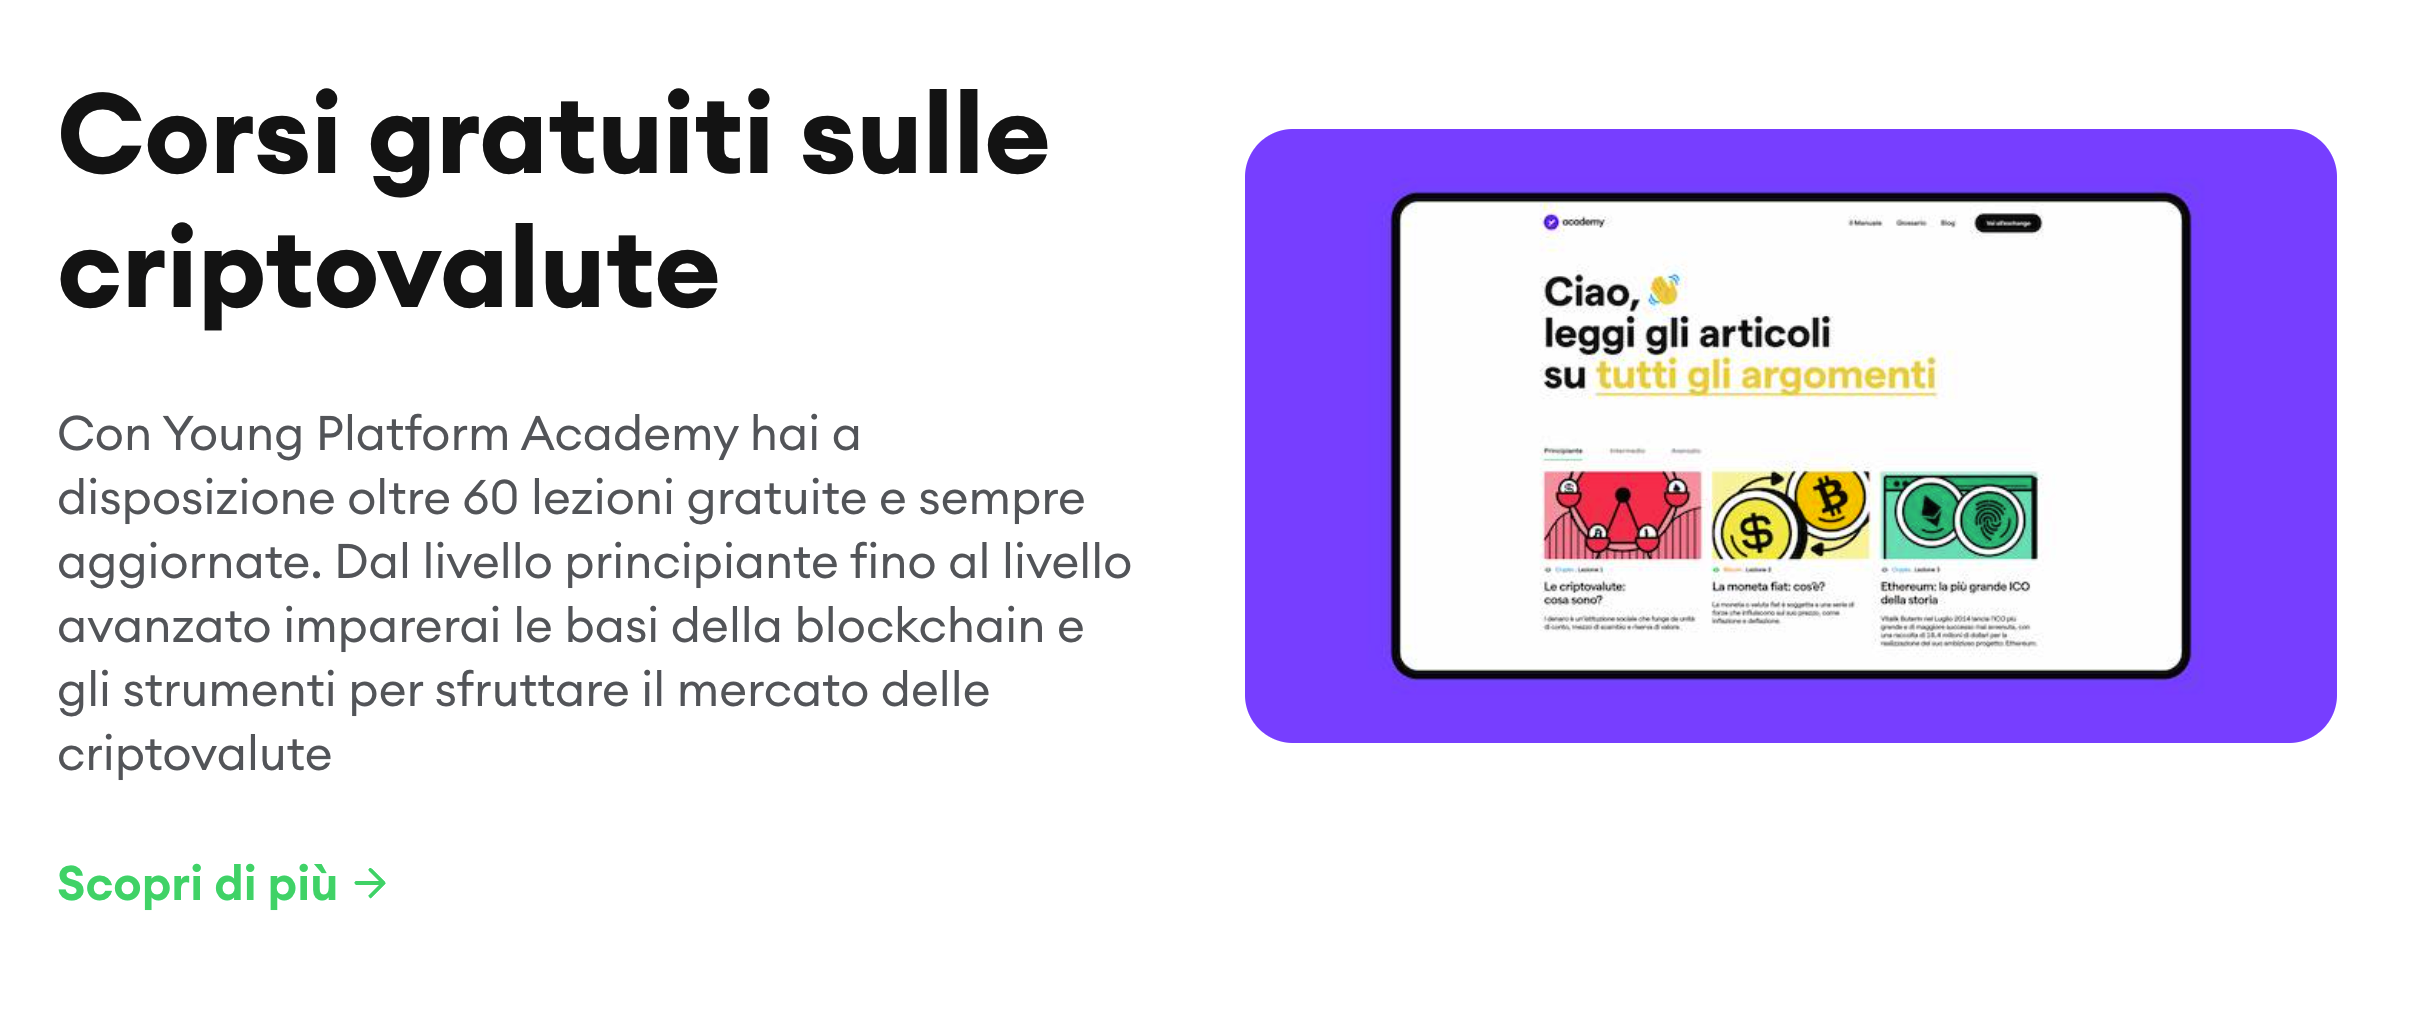
\includegraphics[width=0.80\textwidth]{res/images/internal-pages/support/support-5.png}
  \caption{Sezione che reindirizza all'\textit{Academy}.}
  \label{fig:support-5}
\end{figure}

\begin{figure}[H]
  \centering
  
\includegraphics[width=0.80\textwidth]{res/images/internal-pages/support/support-6.png}
  \caption{Elementi che permettono all'utente di rimanere in contatto 
  con la community (social network e newsletter).}
  \label{fig:support-6}
\end{figure}

L'ultima tipologia di supporto offerta dal sito è la possibilità per 
l'utente di aprire \textit{ticket} all'assistenza. Per fare ciò, è 
presente un bottone \textit{Apri un ticket}, posto in alto a destra, a 
sinistra del bottone verde \textit{Accedi} (fig. \ref{fig:support-1}). 

\paragraph{Who}

Il logo aziendale è sempre presente in alto a sinistra, come illustrato 
nella figura \ref{fig:support-1}.

\paragraph{Where}

Quando l'utente viene reindirizzato a questa pagina, si può notare che si 
è arrivati in un nuovo sottodominio (\textit{support.youngplatform.com}). 
Non è presente però un elemento che permette di ritornare alla pagina a cui 
si è arrivati o per ritornare alla homepage di \textit{youngplatform.com}. 
Per poter tornare alla homepage è necessario recarsi nel footer. Questa 
implementazione è molto svanataggiosa per l'utente e richiede dello sforzo 
per compiere l'azione.

\paragraph{Why}

Indipendentemente dall'esperienza dell'utente, questa pagina è di 
fondamentale importanza, in quanto permette di mettere in contatto 
l'utente con il personale aziendale. Quindi, l'utente vuole prima di 
tutto esplorare questa pagina per vedere se ci sono già delle soluzioni 
illustrate. Per esplorare le soluzioni già proposte dal sito, l'utente 
può visitare le varie soluzioni suddivise per prodotto 
(fig. \ref{fig:support-2}), oppure, utilizzare la barra di ricerca 
(fig. \ref{fig:support-3}). Inoltre, se l'utente non trova la risposta al 
proprio problema, è possibile aprire un nuovo \textit{ticket}.

\paragraph{When}

In questa pagina non è presente alcun riferimento temporale.

\paragraph{How}

Questa pagina è facile da raggiungere dalla homepage. Può essere 
raggiunta tramite il menù principale della homepage 
(fig. \ref{fig:homepage-1}) o tramite il footer (prima voce della quarta 
colonna, fig. \ref{fig:footer}). In questa pagina ci sono delle sezioni 
dedicate per l'esplorazione degli articoli del \textit{Blog} 
(fig. \ref{fig:support-4}), per l'esplorazione degli articoli della 
\textit{Academy} (fig. \ref{fig:support-5}) e per raggiungere i vari 
social network (fig. \ref{fig:support-6}). Inoltre, l'utente può 
esplorare le soluzioni a diversi problemi per ogni prodotto tramite 
una apposita sezione, illustrata in figura \ref{fig:support-3}. Se l'utente 
non trova la risposta la proprio problema, allora il sito offre la 
possibilità di inviare un \textit{ticket} all'assistenza. Per fare ciò, è 
presente un bottone \textit{Apri un ticket}, posto in alto a destra, a 
sinistra del bottone verde \textit{Accedi} (fig. \ref{fig:support-1}). 
Ritengo che, data l'importanza di questa funzionalità, l'elemento che 
permette di aprire un nuovo ticket sia localizzato in un posto errato. 
A primo impatto, tale elemento non è immediatamente riconoscibile e 
pertanto l'utente potrebbe ritrovarsi disorientato (sopratutto se l'utente 
è un principiante). Avrei posto tale elemento in una posizione che lo 
avrebbe reso più visibile, in modo che, anche se l'utente non ne ha 
bisogno, sia ben visibile a prima vista. 